\documentclass[12pt,a4paper,oneside,openright,titlepage]{book}
\usepackage[utf8]{inputenc}
%\usepackage[italian]{babel}
\usepackage{amsmath,amscd}
\usepackage{amsfonts}
\usepackage{amssymb}
\usepackage{natbib}
\usepackage{braket}
\usepackage{caption} % 4 nice captions
\usepackage{amsmath}

\usepackage{bbm} %blackboard numbers


\usepackage{setspace} %per la copertina
\usepackage{graphicx} %per le immagini
\graphicspath{{images/}}



\usepackage{color}		% testo colorato
\usepackage[dvipsnames,table]{xcolor} % testo colorato & sfondo celle tabelle (rimelle)

\usepackage{hyperref}  %s

\usepackage{multirow} %multirow nelle tabelle

\usepackage{gnuplottex} %gnuplot

% SILLABAZIONE

\hyphenation{re-nor-ma-li-za-tion}
\hyphenation{o-pe-ra-tors}
\hyphenation{there-fore}
\hyphenation{li-te-ral-ly}
\hyphenation{cor-res-ponds}
\hyphenation{cor-res-pon-dence}
\hyphenation{cor-res-pon-ding}
\hyphenation{dy-na-mi-cal}
\hyphenation{i-ma-gi-na-ry}
\hyphenation{co-va-riant}
\hyphenation{mo-du-li}
\hyphenation{re-pre-sent-ed}
\hyphenation{phy-si-cal}
\hyphenation{the-o-ries}
\hyphenation{sub-ma-ni-fold}
\hyphenation{ma-ni-fold}
\hyphenation{me-tric}
\hyphenation{e-qui-va-lent-ly}
\hyphenation{existen-ce}
\hyphenation{des-crip-tion}
\hyphenation{des-cribed}
\hyphenation{su-per-gra-vi-ty}
\hyphenation{in-va-riance}
\hyphenation{mi-ni-mal}
\hyphenation{coup-ling}
\hyphenation{coup-lings}
\hyphenation{comp-le-te-ly}
\hyphenation{e-le-gant}
\hyphenation{ap-proxi-ma-ted}
\hyphenation{parti-cu-lar}
\hyphenation{qua-li-ties}
\hyphenation{mo-du-lus}
\hyphenation{ge-ne-ra-lized}
\hyphenation{ge-ne-ral-ly}



%STILE

\linespread{1.2}

% DICHIARAZIONI
% operatore traccia
\DeclareMathOperator{\Tr}{Tr}
%iperboliche

\DeclareMathOperator \ch {ch} 
\DeclareMathOperator \sh {sh} 

%volume

\DeclareMathOperator \vol {vol}

%pder
\newcommand{\pder}[2]{\frac{\partial#1}{\partial#2}}

%real im parts (must be AFTER amsmath, overrides it)
\renewcommand{\Re}{\operatorname{Re}}
\renewcommand{\Im}{\operatorname{Im}}

% string length
\newcommand{\strln}{\ell_s}
\newcommand{\onekten}{\frac{2\pi}{\strln^8}}
\newcommand{\hodge}{\ast}

% ibarj

\newcommand{\ibj}{i\bar{\jmath}}

%spinor conjugate
\newcommand{\scj}[1]{\overline{#1}}

%supersymmetry cursive N

\newcommand{\ssn}{\mathcal{N}}

%normal conjugate representation
\newcommand{\rrep}[1]{\mathbf{#1}}
\newcommand{\cjrep}[1]{\overline{\rrep{#1}}}

%mesonic moduli space
\newcommand{\mmes}{\mathcal{M}_\mathrm{mes}}

% Anti de Sitter
\newcommand{\ads}[1]{\operatorname{AdS}_{#1}}

%TIKZ

\usepackage{tikz}
\usetikzlibrary{arrows,decorations.markings,tikzmark}



%commenti in rosso
\newcommand{\cmmnt}[1]{\textcolor{Mahogany}{\emph{#1}}}


%\ref con parentesi





%FRONT
\author{Riccardo Antonelli}

\setlength\parindent{0pt}
\setlength{\parskip}{0.3cm} 
\begin{document}




\frontmatter


\begin{titlepage}
\begin{center}
 
% Upper part of the page
\includegraphics[scale=.5]{images/logoBlack}
 
\textsc{\LARGE Università degli Studi di Padova}\\[1.5cm]
 
\textsc{\Large Dipartimento di Fisica e Astronomia\\[0.2cm] Corso di Laurea Magistrale in Fisica}\\[2cm]
  
% Title

{\Huge \doublespacing \bfseries \begin{spacing}{1}{Holographic effective field theories: a case study}\end{spacing}}
~\\[4cm]
 
% Author and supervisor
\begin{minipage}{0.4\textwidth}
\begin{flushleft} \large
\emph{Laureando:}\\
Riccardo \textsc{Antonelli}
\end{flushleft}
\end{minipage}
\begin{minipage}{0.4\textwidth}
\begin{flushright} \large
\emph{Relatore:} \\
Luca \textsc{Martucci}
\end{flushright}
\end{minipage}
 
\vfill
 
% Bottom of the page
{\large Anno accademico 2015/2016\\
	\cmmnt{bozza compilata \today}}
 
\end{center}

\end{titlepage}

%\begin{frontespizio}
%\Universita{Padova}
%\Facolta{Scienze Matematiche, Fisiche e Naturali}
%\Corso[Laurea]{Matematica}
%\Titoletto{Tesi di laurea}
%\Titolo{Equivalenze fra categorie di moduli\\
%e applicazioni}
%\Candidato[145822]{Enrico Gregorio}
%\Relatore{Ch.mo Prof.~Adalberto Orsatti}
%\Annoaccademico{19??-19??}
%\end{frontespizio}

%\begin{abstract}

%\lipsum[1]

%\cmmnt{bozza compilata il giorno \today}\\

%\end{abstract}

\thispagestyle{plain}
\begin{center}
   % \Large
   % \textbf{Thesis Title}
    
   % \vspace{0.4cm}
   % \large
   % Thesis Subtitle
    
   % \vspace{0.4cm}
   % \textbf{Author Name}
    
   % \vspace{0.9cm}
    \textbf{Abstract}
\end{center}
The identification of the low-energy effective field theory associated with a given microscopic strongly interacting theory constitutes a fundamental problem in theoretical physics, which is particularly hard when the theory is not sufficiently constrained by symmetries.
Recently, a new approach has been proposed, which addresses this problem for a large class of four-dimensional minimally supersymmetric strongly coupled superconformal field theories, admitting a dual weakly coupled holographic description in string theory. This approach provides a precise prescription for the holographic derivation of the associated effective field theories. The aim of the thesis is to further explore this approach by focusing on a specific model, whose effective field theory has not been investigated so far. \cmmnt{(modificare abstract alla fine del lavoro.)}



\tableofcontents

\mainmatter

\chapter{Introduction}

Strongly-coupled quantum field theories represent canonical examples of physical systems whose study is extremely challenging. Even the question of the mere existence of any interacting QFT in four dimensions from a formal standpoint has not been settled. In addition to this, strong couplings are not amenable to the tools of perturbation theory. The interest in this class of theories stems actually from practical considerations - many of them represent realistic models for physical phenomena, e.g. the theory of strong interaction.

A subset of questions concerns whether a given strongly-interacting theory is described at low energy by an effective local field theory, and if so, what are its degrees of freedom and their precise dynamics. Often, part of the structure of the effective theory is constrained by symmetries, but no general method exists to fix it completely. Recently\cite{MZ}, a novel approach for determining the effective Lagrangian was introduced that makes use of tools from an apparently unrelated area of physics: string theory.

It is remarkable that string theory was originally conceived as a description of hadronic physics, so a low-energy effective theory for what ultimately turned out to be a gauge theory, QCD. When string theory was found to have unsuitable qualities for this application, it was replaced by the theory of quantum chromodynamics - however it also proved to be effective for solving a seemingly unrelated problem of fundamental physics: quantizing gravity. Since then, string theory blossomed into a vast and rich field reaching into numerous areas of mathematics and physics, and of course a candidate for a ``Theory of Everything'' describing the entirety of fundamental physics.

Among the most unexpected discoveries in strings, made decades after their conception, is a series of unusual exact equivalences between string theories set in particular ten-dimensional backgrounds and four-dimensional gauge QFTs. More generally, one finds families of exact equivalences between local quantum field theories and higher-dimensional theories containing gravity, which are termed ``holographic''. This explains the original partial success of strings in modeling strong interactions, assuming that some or perhaps most gauge theories have or can be approximated as having a holographic description as a ten dimensional theory involving strings. This roundtrip has therefore brought strings back to strongly-coupled gauge theories. Various aspects, qualitative and most importantly quantitative, of QFTs can be studied directly by means of their holographic string dual, a gravitational theory, if it exists. 

The first and most important case of such a duality\cite{Maldacena} equates IIB superstring theory set on the background

\begin{equation}
	\operatorname{AdS}_5 \times \mathbb{S}^5
\end{equation}

(the ``bulk'') with maximally supersymmetric Yang-Mills theory on $\mathbb{R}^{1,3}$ (the ``boun\-da\-ry''), which is a conformal field theory. The denomination of ``AdS/CFT'' (anti-de Sitter / conformal field theory) correspondence for holographic dualities stems from this (even though cases either with no AdS geometry or not conformal are known). One direction in which to generalize this construction is to replace $\mathbb{S}^5$ with other compact 5-manifolds $Y_5$. This yields dualities involving more complex and interesting field theories, less constrained by symmetries; therefore this thesis will be focused on this class of correspondences.

Actually, since string theory in general is very challenging to study, AdS/CFT only becomes truly useful in terms of describing the dynamics of the CFT if string theory can be approximated by a weakly coupled effective field theory of its own, supergravity. This limit corresponds to the CFT being strongly-coupled and having a large number of colours. Therefore the regime accessible through holography is precisely the strongly-coupled region where the gauge theory would be normally impossible to investigate.

Recently, a novel approach was introduced\cite{MZ} for determining the effective theory to such duals of $\operatorname{AdS}_5 \times Y_5$. A procedure for identifying the degrees of freedom and the Lagrangian for the effective low-energy theory for a class of gauge theories with $\operatorname{AdS_5} \times Y_5$ holographic duals is provided, by expanding the supergravity action on the dual bulk geometry. Interestingly, these are somewhat special in that they include models of minimal supersymmetry ($\mathcal{N}=1$), which makes for more realistic but by converse less constrained theories than typical holographic field theories, with higher supersymmetry. The ability to pinpoint the exact effective Lagrangian is then particularly noteworthy.

The original contribution in this work is the specialization of this construction to a specific field theory, the $Y^{2,0}$ theory, a strongly-coupled superconformal quiver theory for which we will therefore fix the exact effective Lagrangian, entirely through the geometry of the relative string background. This will require necessarily the determination of the general Calabi-Yau deformation of the background in complex coordinates, which was not known previously.

This thesis will be structured as follows. We will first provide a general introduction to IIB superstring theory, D-brane stacks on cones and the resulting gauge field theories, and holography. Then, we will summarize the relevant results and techniques from \cite{MZ}. Finally, we will present a complete parametrization of the geometry of the $Y^{2,0}$ theory and will apply those results and techniques to identify the exact effective Lagrangian of the field theory.



\chapter{IIB superstrings and branes}


\section{Superstring theory}

String theory either does not admit a nonperturbative Lagrangian formulation, or this formulation is unknown. An action functional can only be written upon choosing a perturbative vacuum; since we anticipate a string theory must include gravity, a choice of vacuum will also require a choice of background metric - in the simplest case Minkowski spacetime. With this choice the action for a string in the simplest case of bosonic string theory is the Polyakov action:

\begin{equation}
S_B = -\frac{T}{2} \int d^2\sigma \sqrt{-g} g^{ab} \partial_a X^\mu \partial_b X_\mu
\end{equation}

where the $D$ fields $X^\mu$ describe the embedding of the string's worldsheet in the $D$-dimensional target spacetime, and the integral is performed over the worldsheet coordinates $\sigma^a = (\tau,\sigma)$. The $X^\mu$ are of course scalars from the point of view of the worldsheet. The auxilary field $g_{ab}$ is a metric on the worldsheet. $T$ instead is a dimensionful constant called the string tension; in fact it is the only free parameter in string theory. We will also often refer to the entirely equivalent quantities $\alpha'$, the Regge slope, and $l_s$, the ``string length'':

\begin{align}
	T = \frac{1}{2\pi\alpha'} && l_s^2 = 2\alpha'
	\label{}
\end{align}


The Polyakov action displays worldsheet diffeomorphism and Weyl invariance, and thus perturbative string theory is naturally a two-dimensional conformal field theory. These symmetries must be quotiented out someway on quantization. The most straightforward way is to eliminate them by fixing a particular gauge and then quantizing (canonical quantization). The three symmetry generators can kill the three degrees of freedom in the metric to fix it to the 2D Minkowski: $g_{ab} = \eta_{ab}$. We get\\

\begin{equation}
S_B = - \frac{T}{2\pi} \int d^2\sigma \partial_a X^\mu \partial^a X_\mu
\end{equation}

where indices are raised with $\eta^{ab}$.\\

There are at least two different approaches to introducing supersymmetry into a string theory. The path followed by the RNS (Ramond-Neveu-Schwarz) formalism is to impose SUSY at the worldsheet level; explicitly, adding fermions $\psi^\mu$ to act as superpartners to the bosons $X^\mu$. The action is extended to

\begin{equation}
S = S_B + S_F = -\frac{1}{2\pi} \int d^2\sigma \partial_a X^\mu \partial^a X_\mu + \bar \psi^\mu \rho^a \partial_a \psi_\mu
\end{equation}

The spinors' equation of motion, the Dirac equation, is actually the Weyl condition in two dimension. This brings the real degrees of freedom in the spinor for each $\mu$ from $4$ to $2$. Recalling that in $(2\bmod 8)$ dimensions there exist Weyl-Majorana spinors satisfying both the Weyl and Majorana conditions, imposing the latter on $\psi$ halves again the on-shell polarizations to $1$. Thus we have a match between bosonic and fermionic degrees of freedom. It can be proven the theory above is indeed worldsheet supersymmetric.\\

To quantize canonically, we introduce canonical commutation/anticommutation relations:

\begin{align}
[X^\mu(\sigma),X^\nu(\sigma')] = \eta^{\mu\nu} \delta^2(\sigma-\sigma') && \{\psi^\mu(\sigma),\psi^\nu(\sigma')\} = \eta^{\mu\nu} \delta^2(\sigma-\sigma')
\end{align}

Note the $X^0$ and $\psi^0$ would create negative norm states, but these modes are eliminated by resorting to superconformal invariance. Classically this symmetry imposes the stress-energy tensor $T^{\mu\nu}$ and the supercurrent $J^a_\alpha$ vanish; imposing that in the quantum theory they annihilate physical states yields the restriction that removes the longitudinal ghosts from the spectrum. These take the name of super-Virasoro constraints.\\

Then the procedure for building the string spectrum is to expand the classical solutions in terms of Fourier modes, identify creators and destructors, and then select the states of the Fock basis that satisfy the super-Virasoro constraints.\\

Boundary conditions for $\psi^\mu$ for an open string can actually be satisfied in two different by imposing periodicity or antiperiodicity, giving rise to the NS (Neveu-Schwarz) and R (Ramond) sectors, built over two grounds $\ket{0}_{NS}$ and $\ket{0}_R$. Closed strings have four: $\ket{0}_{NS-NS}$, $\ket{0}_{R-R}$, $\ket{0}_{R-NS}$, $\ket{0}_{NS-R}$ corresponding with different choice periodicity conditions for left and right-movers.

\subsection{Open strings}

It can be shown that while the NS ground $\ket{0}_{NS}$ is unique, and thus a spacetime scalar, $\ket{0}_R$ is eight-fold degenerate and this 8-plet transforms under the spinor representation of transverse $SO(8)$ - in other words, it's a spacetime spinor. In particular, it's a chiral Weyl-Majorana spinor, so it can be taken to be either of positive or negative chirality, choices we will denote as $\ket{+}_R$, $\ket{-}_R$.\\

The spectrum is built by acting on one of the grounds with bosonic and fermionic creators, to obtain states of higher and higher mass. For the NS sector, there are bosonic creators $a_n^{i\dagger}$ ($n\geq 1$) and fermionic $b_r^{i\dagger}$ ($r$ positive half-integer), and the mass of the excited string is given by:

\begin{equation}
	\alpha' M^2 = \sum_{n=1}^\infty n \,a_n^{i\dagger} a_n^i  + \sum_{r=1/2}^\infty r b_r^{i\dagger} b_r^i - \frac{1}{2}
	\label{}
\end{equation}

while for the R sector the fermionic creators are replaced by the integer-indexed $d_n^{\dagger i}$:

\begin{equation}
	\alpha' M^2 = \sum_{n=1}^\infty \left(n\, a_n^{i\dagger} a_n^i + n d_n^{i\dagger} d_n^i \right)
	\label{}
\end{equation}

The $i$ indices here are target spacetime transverse indices, $i=1,\cdots,8$. Therefore each creator increases the spin of the string by one unit.\\

It's worrying that the mass-shell formula above assigns a negative mass-squared to the NS ground, which is therefore a tachyon. In addition, it's the \emph{only} tachyon, meaning this theory is not spacetime supersymmetric. We will see in the next section how this state is actually removed and target supersymmetry recovered. For now, we note the only massless states are

\begin{equation}
	b_1^{i\dagger} \ket{0}_{NS} \quad \quad \ket{+}_{NS}
	\label{}
\end{equation}

while the rest of the tower of states have Planck-large $\sim (\alpha')^{-1/2}$ masses. The former state is a massless spin-$1$ boson, so it must be a photon associated with a $U(1)$ gauge theory. The latter is its spin-$1/2$ superpartner, a photino.

\subsection{GSO projection}

The construction above does not define a consistent theory. This is in part because it's not spacetime supersymmetric, an essential requirement considering that, as will be seen shortly, the closed string spectrum includes a gravitino (a massless spin-$3/2$ state) which must be associated with local supersymmetry. A procedure known as the Gliozzi, Scherk, Olive (GSO) projection solves this issue and in addition also eliminates the tachyonic state $\ket{0}_{NS}$.\\

The following operator is introduced, acting on the NS sector as

\begin{equation}
	G = (-1)^{1+\sum_r b_r^{i\dagger} b_r^i} = (-1)^{\hat F + 1}
	\label{}
\end{equation}

and on the R sector as

\begin{equation}
	G = \Gamma_{11}(-1)^{\sum_r d_r^{i\dagger} d_r^i} = \Gamma_{11} (-1)^{\hat F}
	\label{}
\end{equation}

$\hat F$ is the worldsheet fermion number, and $\Gamma_{11} = \Gamma_0 \cdots\Gamma_9$ gives the chirality of the state.\\

Then the spectrum is projected into the $G=1$ subspace for the NS sector, and into $G=\pm1$ (either choice works) for the R sector. These two choices correspond to keeping either $\ket{+}_R$ or $\ket{-}_R$ respectively and discarding the other.\\

When amputated with this precise prescription the spectrum is found to be spacetime supersymmetric. The scalar tachyon $\ket{0}_{NS}$ in particular is eliminated, being $G$-odd.


\subsection{Closed strings}

The closed string spectrum, in somewhat poetic language, is the ``square'' of the open string spectrum. As seen before the choice can be made for either NS or R boundary conditions separately for left-movers and right-movers, giving four sectors. The GSO projection is performed separately on left and right movers, so that one is presented with the choice of the relative chirality of the two projections and so of the R grounds. These two possibilities will actually result in two different string theories. Choosing opposite chiralities gives type IIA strings, whose massless spectrum is given by

\begin{align}
	\tilde b_{1/2}^{i\dagger} \ket 0_{NS} &\otimes b_{1/2}^{j\dagger}\ket{0}_{NS} \\
	\tilde b_{1/2}^{i\dagger} \ket 0_{NS} &\otimes \ket{+}_{R}\\
	\ket{-}_R &\otimes b_{1/2}^{j\dagger}\ket{0}_{NS}\\
	\ket{-}_R &\otimes \ket{+}_R
	\label{}
\end{align}

(the $\sim$ distinguishes creators/destructor for left movers from right movers). And IIB strings arise from equal chiralities:


\begin{align}
	\tilde b_{1/2}^{i\dagger} \ket 0_{NS} &\otimes b_{1/2}^{j\dagger}\ket{0}_{NS} \\
	\tilde b_{1/2}^{i\dagger} \ket 0_{NS} &\otimes \ket{+}_{R}\\
	\ket{+}_R &\otimes b_{1/2}^{j\dagger}\ket{0}_{NS}\\
	\ket{+}_R &\otimes \ket{+}_R
	\label{}
\end{align}

So the massless spectrum is composed of $4$ sectors of $64$ physical states, two of them bosonic (NSNS, and RR) and the other fermionic (RNS and NSR). Massless states will correspond to fields in the supergravity approximation, in which the massive modes of the string decouple and the string theory is well described by the corresponding variety of 10D supergravity.\\

%~\\\cmmnt{Review molto rapida dei creatori e distruttori nei quattro settori, formula di massa e spettro massless. Proiezione GSO}

\section{Type II supergravity and D-brane content}

%\cmmnt{Proiezione GSO per le tipo II; chiralità dei fermioni; potenziali RR e p-form electrodynamics; D-brane corrispondenti. Magari T \& S duality?}

%\section{From 11D SUGRA to type IIB SUGRA}

At scales much lower than the Planck scale (equivalently: when the curvature radii are $\gg$ than the string size), all massive modes of a string theory decouple and a good description is given by an effective field theory comprising only the massless excitation. Since the string length goes to zero in this limit strings in massless states are essentially pointlike and the quantum theory will correspond to a local quantum field theory.\\

The effective field theories of the five superstring theories are the five supergravity (SUGRA) theories in $10$ dimensions. The name of each SUGRA coincides with that of the superstring theory it's the effective theory of (e.g., IIB SUGRA is the effective theory of IIB superstrings). Supergravities are supersymmetric theories containing general relativity. Just like Einstein gravity, they are nonrenormalizable, reflecting their origin as effective theories. As field theories, they are considerably simpler than general strings to find background solutions to; therefore we will make extensive use of the supergravity approximation in the context of holography.\\

$10D$ SUGRAs are perhaps easier to introduce starting instead from the unique $11D$ SUGRA. The field content of $11D$ SUGRA is as follows (number of physical polarizations in parentheses):

\begin{itemize}
\item graviton $g_{MN}$ ($44$)
\item 3-form $A_3$ ($84$)
\item Majorana gravitino $\psi_M$ ($128$)
\end{itemize}

As required by supersymmetry, the number of on-shell boson and fermion states are equal. These states form an irreducible supermultiplet, a gravity multiplet.

Upon dimensional reduction on a circle, in $10D$ these fields decompose into those of type IIA SUGRA:

\begin{itemize}
\item graviton $g_{\mu\nu}$ ($35$), Kalb-Ramond 2-form $B_2$ ($28$), dilaton $\phi$ ($1$)
\item 1-form $A_1$ ($8$), 3-form $A_3$ ($56$)
\item two Weyl-Majorana gravitinos of opposite chirality $\psi_\mu$ ($56$ each), two Weyl-Majorana dilatinos of opposite chirality $\lambda$ ($8$ each)
\end{itemize}

These are respectively the NSNS, RR, and NSR + RNS massless modes.\\

Obviously, again we find that the total bosonic states are $35+28+1+8+56 = 128$ and the fermions $2\cdot (56+8) = 128$. This is a theory with $\mathcal{N}=(1,1)$ SUSY, meaning there's two Weyl-Majorana (we recall again the existence of Weyl-Majorana fermions in $D=10$) SUSY generators of opposite chirality.\\

We will mainly be interested, however, in type IIB SUGRA, which is not obtainable from dimensional reduction, but rather is the T-dual of type IIA. The field content is as follows:

\begin{itemize}
\item graviton $g_{\mu\nu}$ ($35$), Kalb-Ramond 2-form $B_2$ ($28$), dilaton $\phi$ ($1$)
\item 0-form $A_0$ ($1$), 2-form $A_2$ ($28$), 4-form $A_4$ with self-dual field strength ($35$)
\item two Weyl-Majorana gravitinos of equal chirality $\psi_\mu$ ($56$ each), two Weyl-Majorana dilatinos of equal chirality $\lambda$ ($8$ each)
\end{itemize}

Again, these are respectively the NSNS and RR bosons, and the NSR+RNS fermions. IIB SUGRA has $\mathcal{N}=(2,0)$ supersymmetry.\\

This net of relationships between SUGRAs in $10$ and $11$ dimension is actually the effective limit of dualities between string/M-theories of which these SUGRAs are effective field theories. The relevant part of the scheme is as follows:

\[\begin{CD}
\text{"M-theory"}     @> \text{dim. red. on }\mathbb{S}^1>>  \text{IIA strings} @> \text{T-duality} >> \text{IIB strings} \\
@VV\text{eff. th.}V        @VV\text{eff.th.}V  @VV \text{eff.th.} V\\
\text{11D SUGRA}     @> \text{dim. red. on }\mathbb{S}^1>> \text{IIA SUGRA} @> \text{T-duality}>>  \text{IIB SUGRA}
\end{CD}\]
\\
In both IIA and IIB, the RR sector admits the following gauge transformations:

\begin{align}
B_2 \rightarrow B_2 + d\Lambda_1 && A_p \rightarrow A_p + d\Lambda_{p-1} - H_3 \wedge \Lambda_{p-3}
\end{align}

for any set of arbitrary k-forms $\Lambda_p$, leaving invariant the field strengths:

\begin{equation}
\begin{aligned}
H_3 &:= dB_2 \\
F_{p+1} &:= dA_p + H_3 \wedge A_{p-2} \label{fieldstrengths}
\end{aligned}
\end{equation}

Where $A_{p}$ with $p<0$ is set to $0$. Now, the RR potential $A_{p}$ obviously couples to $D(p-1)$-branes by an interaction term which is the integral of $A_{p}$ over the worldvolume; this is an electric coupling of the $D(p-1)$-brane to $F_{p+1}$. The coupling however could also be magnetic, electric-magnetic duality being implemented in general through Hodge duality. We define $F_p$ for additional values of $p$ through

\begin{equation}
F_{9-p} = \widetilde\star F_{p+1}
\end{equation}

note that for the IIB $F_5$ this is actually a constraint. The new field strengths can then be locally trivialized as of \ref{fieldstrengths} and so we end up with a complete set of potentials $A_0, \ldots A_8$ for IIB and $A_1 \ldots A_9$ for IIA. The duality between potentials would be given by $A_p \leftrightarrow A_{8-p}$, and if $D(p-1)$-branes couple electrically to $A_p$, then $D(7-p)$-branes couple magnetically to it, that is to say electrically to $A_{8-p}$.\\

Therefore, the magnetic dual to a $Dp$-brane is a $D(6-p)$-brane.

\section{Action functional for IIB SUGRA}

There is a considerable obstacle to a covariant (i.e. explictly supersymmetric) formulation of type IIB supergravity in the self-duality constraint for the field strength 5-form $\tilde{F}_5$. We will take the common path of formulating the Lagrangian theory ignoring the constraint (and thus in excess of bosonic polarizations with respect to an explicity supersymmetric theory) and then imposing self-duality by hand after deriving the equations of motion. Therefore the action will not be supersymmetric itself, while the Euler-Lagrange equations augmented with the constraint will be.\\

Actually, for the purpose of building classical solutions, where spinor fields vanish anyway, the fermionic sector of the action will not be important. The bosonic sector is as such:

\[ S_B = S_{NS} + S_R + S_{CS} \]

where $S_{NS}$ is the action relevant to the fields originally from the superstring NS-NS sector:

\[ S_{NS} = \frac{1}{2\kappa^2} \int d^{10} x \sqrt{-g} \, e^{-2\phi} \left( R + 4 \partial_\mu \phi \partial^\mu \phi - \frac{1}{2} | H_3 |^2 \right) \]

Then $S_R$ is for R-R fields, essentially just kinetic terms for the $A$ forms:

\[ S_R = -\frac{1}{4\kappa^2} \int d^{10} x \sqrt{-g} 
\left(| F_1 |^2 + | \tilde{F}_3 |^2 + | \tilde{F}_5 |^2 \right)\]

And finally we supplement with a Chern-Simons type term:

\[ S_{CS} = -\frac{1}{4\kappa^2} \int A_4 \wedge H_3 \wedge F_3 \]

note the untilded $F_3$. This is evidently a purely topological term.


\section{D-brane action}

D-branes appear as nonperturbative objects in string theories. They are themselves dynamical and the dynamics are modeled in the string perturbative regime by an action functional\cite{ibanezU}. To formulate the action, we introduce coordinates $\sigma^a$ on the $(p+1)$-dimensional worldvolume $W$ and functions $X^\mu(\sigma^a)$ describing the embedding of $W$ in spacetime. \\

Open strings can exist with their endpoints on D-branes. With a single D-brane, the massless open string modes with endpoints on the brane include a $U(1)$ gauge field $A$, with field strength $F$.\\

The bosonic part of the D$p$-brane action is:

%\begin{equation}i
%	S = - T_{Dp} \int d^{p+1}\sigma \sqrt{ - \det \left( G_{ab} \right) }
%	\label{}
%\end{equation}

\begin{align}
	S_{Dp} = & -\mu_{Dp} \int_W d^{p+1}\sigma e^{-\phi} \sqrt{ - \det \left( X^{*}(g - B_2) - 2\pi\alpha' F \right)} \label{actionDBI}\\
& + \mu_{Dp} \int_W \left[ X^{*}\left(\sum_k C_k \right) \wedge e^{2\pi\alpha'F-B_2} \wedge (1 + \mathcal{O}(R^2))
\right]_{p+1} 	\label{actionCS}
\end{align}

Where 

\begin{equation}
	\mu_{Dp} = \alpha'^{\,-\frac{p+1}2}(2\pi)^{-p}
	\label{}
\end{equation}

The first line \ref{actionDBI} is the Dirac-Born-Infeld action and generalizes the Nambu-Goto action; the notation $X^*(T)$ denotes the pull-back of a spacetime tensor to the worldsheet. For example, if $B = F = 0$, $X^*(g)$ is the induced metric $h_{ab} = \partial_a X^\mu \partial_b X^\nu g_{\mu\nu}$. Setting only $B=0, \phi = \mathrm{const}$ and expanding $S_{DBI}$ in powers of $\alpha'$:

\begin{equation}
	S_{DBI} = -\frac{\mu_{Dp}}{g_S} \int_W d^{p+1} \sigma \sqrt{-h} + \frac{\alpha'^{-(p-3)/2}}{4 g_s (2\pi)^{p-2} } \int_W d^{p+1} \sigma \sqrt{-g} F_{\mu\nu} F^{\mu\nu} + \dots
	\label{DBIexpanded}
\end{equation}

the first term is the direct generalization of the Nambu-Goto action, allowing us to identify the D$p$-brane tension $T_{Dp} = \frac{\mu_{Dp}}{g_S}$. The second is a Yang-Mills action for the $U(1)$ gauge field, restricted to the worldvolume.\\

The second line \ref{actionCS} is a Chern-Simons type term coupling the brane to the RR potentials. The sum over $k$ only spans odd or even respectively for IIA or IIB, and the $\left[ \; \right]_{p+1}$ notation means the $p+1$-form component must be selected so as to define a meaningful integral. We note that in vanishing $B_2$ and curvature, and expanding in $F$, the physical interpretation becomes less obscure:

\begin{equation}
	S_{CS} = \mu_P \int_W C_{p+1} + \mu_P(2\pi\alpha') \int_W C_{p-1} \wedge F + \mathcal{O}(F^2)\label{} \end{equation}

so that there is a direct, standard coupling of the $C_{p+1}$ potential to the D$p$-brane at the zeroth order in $F$. Higher order terms mean a coupling with the lower RR potentials and are due to nontrivial $F$ configurations which induce lower-dimensional D-brane charges localized inside the D$p$-brane.

%\subsection{D-brane stacks}

\label{sec:branestacks}

We touch briefly upon the easy generalization of the above action to the case of $N$ coincident D$p$-branes, a ``stack''. The salient point is the extension of the gauge group from $U(1)$ to $U(N)$. The gauge bosons in the adjoint representation with indices $i\bar j$ come from massless modes of open strings stretching between brane $i$ and brane $\bar j$. Essentially, the $F^2$ term (and higher) in \ref{DBIexpanded} must be supplemented with gauge traces.

%\cmmnt{stack D-brane, YM non abeliana}



\chapter{D3-brane stacks on Calabi-Yau cones}

\label{chap:cones}One of the most essential ingredients for the conception of the idea of holography was the fact that a stack of coincident D3-branes naturally features a 4D gauge theory on their world-volume, where the 4D fields emerge from the modes of open strings stretching between them. In the simplest and most famous example, a stack of $N$ D3-branes is placed in otherwise Minkowski $\mathbb{R}^{1,9}$; the corresponding field theory is the maximally supersymmetric Yang-Mills in four dimensions (SYM4).

Setting the stack on a different background geometry instead gives rise to a large family of different field theories; a particularly interesting subset is given by spacetimes of the form

\begin{equation} 
	M = \mathbb{R}^{1,3} \times X_6 \,,
\end{equation}

where the $\mathbb{R}^{1,3}$ is parallel to the branes (and must be identified with the field theory spacetime) and $X_6$ is a 6-dimensional Calabi-Yau cone over a compact 5-fold base $Y_5$. By $X_6$ being a cone it is meant there exists a conical radial coordinate $r$ such that the metric on $X_6$ is of the form

\begin{equation}
	ds^2 = dr^2 + r^2 ds_5^2
	\label{}
\end{equation}

With $ds_5^2$ the metric on $Y_5$.

In this language, the SYM4 example above corresponds to $X_6 = \mathbb{R}^6 = \mathbb{C}^3$, which is (trivially) a cone over $Y_5 = \mathbb{S}^5$. This is the only case where $X_6$ turns out to be smooth; in general it will feature a conical singularity in the origin. The motivation for jumping so hastily to a generalization as radical as a singular spacetime, instead of other smooth spacetimes, is that the latter will not actually introduce any novel features. As will be clarified in a holographic context (see for example section \ref{sec:holography}), the flow towards the IR of the field theory will actually correspond to ``zooming in'' on the D-branes, and any smooth spacetime will converge to flat $\mathbb{R}^6$ in this limit. Only a genuine singularity is going to introduce any novel behaviour in the IR field theory, and conical defects are a well-known example of singularities on which string theory is known to be formulable\cite{idk}.

Non-trivial choices for the base will typically yield theories with reduced (even minimal) supersymmetry, which are considerably more challenging to study.

In this chapter, we will first describe some general features of the theories resulting from the placement of D3-branes on these conical backgrounds. Then, we will concentrate in particular on a specific chain of field theories starting from the simplest example of SYM4 and ending up on the $Y^{2,0}$ theory, the study of which is the main objective of this work.

\section{Superconformal field theory}\label{sec:scft}

We now provide a short introduction to 4D conformal field theories, their supersymmetric variants, and the relevant terminology.

%For a given $d$-dimensional spacetime with metric $g_{\mu\nu}$, conformal transformations are defined to be diffeomorphisms $x^\mu \rightarrow x'^\mu$ which leave the metric unchanged in form up to an $x$ dependent scalar function (a conformal factor):
%
%\begin{equation}
%%	ds'^2 = g'_{\mu\nu}(x') dx'^\mu dx'^\nu = \Omega(x) g_{\mu\nu}(x) dx^\mu dx^\nu
%	ds^2 \rightarrow ds'{}^2 = \Omega(x) ds^2,
%	\label{}
%\end{equation}
%
%or, equivalently:
%
%\begin{equation}
%	g'_{\mu\nu}(x') = \Omega(x) g_{\mu\nu}(x).
%	\label{}
%\end{equation}

Consider flat spacetime of dimension $d$ and signature $p,q$, with $p+q = d$. Take a coordinate chart $x^\mu$ in which the metric takes the standard form $\eta_{\mu\nu}$. Conformal transformations are defined to be diffeomorphisms $x^\mu \rightarrow x'^\mu$ which leave the metric unchanged in form up to an $x$ dependent scalar function (a conformal factor):

\begin{equation}
	g'_{\mu\nu}(x') = \Omega(x) \eta_{\mu\nu}\,.
	\label{}
\end{equation}

%The group of these transformations is known as the conformal group associated with the metric. Our case of interest is flat spacetime\footnote{to be precise, the conformal group is clearly equal for two metrics that are conformally equivalent ($g_{\mu\nu} = e^{\phi(x)} h_{\mu\nu}$), so that the group essentially depends only on the conformal class of the manifold. Therefore, what we will find for $\mathbb{R}^{1,D-1}$ will apply equally to all conformally flat metrics.}, $g_{\mu\nu} = \eta_{\mu\nu}$, and the corresponding group is commonly known as \emph{the} conformal group.

These maps form evidently a group, which is known as the conformal group $CO(p,q)$. We will mainly be interested in $CO(1,d-1)$, but most of what we will now show applies in general signatures.

In $d>2$, the conformal group will turn out to be a finite-dimensional Lie group, of which we specify now the connected component. An obvious subgroup is maps that leave the metric unchanged, so Poincar\'e transformations, with generators $P_\mu$ and $J_{\mu\nu}$. A second easy guess is the subgroup with constant conformal factors, that is scale transformations or dilations

\begin{align}
	x^\mu \rightarrow \lambda x^\mu && \eta_{\mu\nu} \rightarrow \lambda^{-2} \eta_{\mu\nu}
	\label{}
\end{align}

whose generator is called $D$. To generate the whole conformal group a final class of transformations must be introduced, special conformal transformations, generated by $K_\mu$ and with finite action\footnote{It should be noted special conformal transformations are not well-defined on $\mathbb{R}^{p,q}$, as the denominator can vanish. Indeed, these more naturally act on the conformal compactification $\overline{\mathbb{R}^{p,q}}$, including points at infinity.}

\begin{equation}
	x^\mu \rightarrow \frac{x^\mu - b^\mu x^2}{1-2 b^\nu x_\nu + b^2 x^2}
	\label{}
\end{equation}

Together, $P_\mu$, $J_{\mu\nu}$, $D$ and $K_\mu$ generate the connected component of the conformal group in $D$ dimensions. The extension of the Poincar\'e algebra to the conformal one is characterized by the following additional commutators (using hermitian generators)

\begin{align}
	[J_{\mu\nu},K_\rho] 	&= 2i \eta_{\rho[\mu} K_{\nu]}	\label{kisvector}\\
	[J_{\mu\nu},D] 		&= 0 				\label{disscalar}\\
	[D, P_\mu] 		&= i P_\mu 			\label{pisraising}\\
	[D, K_\mu] 		&= -i K_\mu			\label{kisraising}
\end{align}

Equations \eqref{kisvector} and \eqref{disscalar} just confirm $K_\rho$ is a vector and $D$ is a scalar. \eqref{pisraising} and \eqref{kisraising} instead state that $P_\mu$ and $K_\mu$ are respectively raising and lowering operators for $D$. It is worth of notice that this group is actually $SO(2,D)$, the Lorentz group in mixed signature $(2,D)$. This can be shown by combining the generators in

\begin{equation}
	J_{MN} = 
	\begin{pmatrix}
		J_{\mu\nu} 		& (K_\mu - P_\mu)/2	& - (K_\mu+P_\mu)/2 \\
		(P_\mu - K_\mu)/2	& 0			& D \\
		(K_\mu+P_\mu)/2		& -D			& 0
	\end{pmatrix}
	\label{}
\end{equation}

and then it can be verified that $J_{MN}$ satisfy the algebra of $\mathfrak{so}(2,D)$. This equivalence will be relevant when we will introduce AdS/CFT, since $SO(2,D)$ is also the isometry group of $AdS_{D+1}$.

A quantum field theory which has the conformal group as symmetries is called a conformal field theory (CFT). In such a theory, particles lie in irreducible representations of the conformal group; since the mass $P^2$ is not a Casimir for the whole group, it becomes useful to replace it with more relevant quantum numbers. Consider the dilation operator: in the quantum theory it will be represented by

\begin{equation}
	D = -i (x^\mu\partial_\mu + \Delta)
	\label{}
\end{equation}

where $\Delta$ gives the intrinsic scaling dimension of a field, which will in general transform as $\phi(x) \rightarrow \lambda^{\Delta} \phi(\lambda x)$. $\Delta$ is therefore a good quantum number. Considering the role of $P$ and $K$ as ladder operators, changing the conformal dimension by $\pm 1$, we can deduce states will come in multiplets of ever-increasing dimension $\Delta_{(0)} + n$, $n\geq 0$, and that the lowest-dimension state will be annihilated by $K_\mu$. Fields in the kernel of $K_\mu$ will be called primary, and others, obtained by applying powers of $P_\mu$ (hence, derivatives) will be called descendants.

A primary field is then identified by its conformal dimension and its representation under the Lorentz group, so, now specializing to $D=4$, by quantum numbers $(\Delta,j_L,j_R)$. We recall Lorentz irreps are indexed by two half-integers $(j_L,j_R)$, for example: $(0,0)$ is a scalar, $(\frac{1}{2},0)$ and $(0,\frac{1}{2})$ are left/right Weyl spinors, $(\frac{1}{2},\frac{1}{2})$ is a vector, and so on.

A classically conformal field theory very often fails to be conformal when quantized. This happens because the dilation symmetry is anomalous. Classical scale invariance clearly implies all couplings are adimensional; in the quantum theory these couplings $g^i$ will run under renormalization with a corresponding $\beta$ function, as in

\begin{equation}
	\frac{dg^i}{d\ln\mu} =: \beta^i(g)\,.
	\label{}
\end{equation}

The dependency of the running coupling on the energy scale, or equivalently the creation of a mass scale by dimensional transmutation, means the conformal symmetry is spoiled\footnote{We are here using conformal and scale (i.e. dilation) invariance interchangeably, but they are not identical. Conformal symmetry obviously includes dilations, but scale invariance $+$ Poincar\'e does not generate the whole conformal group, as special conformal transformations are independent. Scale invariant but not conformal theories are known explicitly\cite{scalebutnotconf}, but they are rare. We will work with the assumption dilation-invariant $\Rightarrow$ conformal.}. This happens for example in quantum chromodynamics, a classically conformal theory with a scale anomaly giving rise to the $\Lambda_\text{QCD}$ mass scale, or quantum electrodynamics where the scale is at the Landau pole. Since the Noether current corresponding to dilations is the trace of the energy-momentum tensor, the anomaly will be detectable by the appearence of a nonzero matrix element $\langle T^{\mu}_{\;\,\mu} \rangle \propto \beta(g) \neq 0$.

Only if all the $\beta$ functions vanish identically, i.e. if the theory is finite, is quantum conformal invariance guaranteed. We will encounter an example of such a theory in section \ref{SYM4}. Otherwise the theory will only be conformal for specific values of the $g^i$ at which all the $\beta$ functions vanish, that is to say at fixed points. In general a quantum field theory will flow under renormalization from a non-conformal point towards an attracting IR fixed submanifold, the locus of $\left\{ \beta^i(g) = 0 \right\}$, called the conformal manifold.

An important point is that after the theory has regained its classical conformal symmetry after converging through RG flow to an IR fixed point, the quantum scaling dimensions $\Delta$ of operators will not coincide with the original value they had in the classical theory, the canonical dimension $\Delta_0$. They will be modified by quantum corrections that add an anomalous dimension

\begin{equation}
	\Delta = \Delta_0 + \gamma(g_*)\,,\quad \gamma(g) = - \frac{1}{2}\frac{d \ln Z}{d \ln\mu},
	\label{}
\end{equation}

where $\sqrt Z$ renormalizes the wavefunction\footnote{It should be noted some authors prefer to define $\gamma = - \frac{d\ln Z}{d \ln \mu}$. In addition, $Z$ is generally a matrix that mixes different fields together under RG flow; however in all of the cases considered in this work this can be ignored, since only fields in the same gauge representation and with the same spin could ever mix, and those will always turn out to be connected by a flavour symmetry.}, and $g_*$ are the values of the couplings at the conformal fixed point.

Having introduced the extension of the Poincar\'e group to $SO(2,4)$, we would like to press this further to include supersymmetry. Supersymmetry is implemented by adding $\mathcal{N} \leq 4$ Weyl supercharges $Q^A$, $\scj{Q}_A$ ($A=1,\ldots,\mathcal{N}$) to generate the super-Poincar\'e supergroup $\operatorname{ISO}(1,3|\,\mathcal{N})$. The superconformal group $SO(2,4|\,\ssn)$ is then the minimal supergroup containing both. The first important feature is that a second set of supercharges $S_A$, $\scj{S}^A$ must be introduced to close the algebra, since

\begin{align}
	[K_\mu , Q^A] = - \sigma_\mu \scj{S}^A\,, && [P_\mu, S_A] = \scj{Q}_A  \scj\sigma_\mu \,;
	\label{}
\end{align}

so that superconformal symmetry $SO(2,4|\,\mathcal{N})$ involves twice as many supercharges as normal supersymmetry for a given $\mathcal{N}$. Another relevant excerpt from the table of commutators (which we do not reproduce in full) states $Q^A$ and $S_A$ are also ladder operators for dilations,

\begin{align}
	[D,Q^A] = \frac{i}{2} Q^A\,, && [D,S_A] = - \frac{i}{2} S_A\,,
	\label{}
\end{align}

raising and lowering the dimension $\Delta$ by $\pm 1/2$. In a superconformal field theory (SCFT) we then expect multiplets of dimension $\Delta = \Delta_0 + \frac{n}{2}$. Primary operators must now be annihilated by both $K_\mu$ and $S_A$, and are classified again by dimension and spin $(\Delta,j_L,j_R)$ but also by the $U(1)\times SU(\mathcal{N})$ R-symmetry quantum numbers $(R,\mathbf{r})$ ($\mathbf{r}$ denoting a generic irrep of $SU(\ssn)$). Then, by acting with the raising operator $Q^A$ charges one can reconstruct a finite-dimensional supermultiplet, as in normal supersymmetry. Instead, powers of $P_\mu$ reconstruct the infinite ladder of derivatives forming an infinite-dimensional representation of the conformal group; these can be recombined into a field by Taylor expansion. In conclusion, an infinite-dimensional representation of the superconformal group can be organized into a superfield

\begin{equation}
	\Phi_{\ldots} (x^\mu , \theta^A, \scj\theta^A)
	\label{}
\end{equation}

where $\ldots$ stands for Lorentz and R-charge-$SU(\ssn)$ indices for the primary.

Actually, not all values for $\Delta$ are allowed in a quantum theory. Imposing physical states have non-negative norm (i.e., unitarity) results in lower bounds for the quantum scaling dimension\cite{unitarity},

\begin{equation}
	\Delta \geq f(j_1,j_2)\,;
	\label{}
\end{equation}

moreover, since violation of the bound results in negative norms, by continuity when it is saturated zero-norm states appear. This correspond in general to a shortening of the multiplet, which becomes constrained to be annihilated by a polynomial of $P_\mu$. For example, for scalar fields

\begin{equation}
	\Delta \geq 1
	\label{uniboundscalar}
\end{equation}

and $\Delta = 1$ iff $\partial_\mu \partial^\mu \Phi = 0$, that is, $\Phi$ is free. In the spin-1 case, $\Delta \geq 3$ and equality holds only if the field is a conserved current ($\partial_\mu J^\mu = 0$); for spin-2 $\Delta \geq 4$ and $\Delta = 4$ only if $\partial_\mu T^{\mu\nu} = 0$, that is to say $T^{\mu\nu}$ must be the stress-energy tensor. This result implies in particular that conserved operators must have fixed, canonical dimension and so are not renormalized.

In $\ssn \geq 1$ SCFTs, more interesting unitarity bounds can be introduced by extending the above reasoning to include superconformal symmetries. Introducing the $U(1)$ R-charge symmetry (and normalizing such that $R_Q = 1$), one is led to bounds of the type

\begin{equation}
	\Delta \geq f(j_1,j_2,R)
	\label{}
\end{equation}

depending also on the R-charge of the superfield. Saturation corresponds to the appearance of ghosts and a shortening of the multiplet, which is annihilated by a polynomial of $P_\mu$ and $Q$. In particular, for scalars

\begin{equation}
	\Delta \geq \frac{3}{2} R
	\label{}
\end{equation}

and equality holds iff $\overline D_{\dot\alpha} \Phi = 0$, i.e. if the superfield is chiral. Thus, chiral fields will satisfy

\begin{equation}
\Delta = \frac{3}{2} R\,. \label{deltarcharge}
\end{equation}


\section{General features of D3-brane on Calabi-Yau cones}\label{sec:generalcones}

We consider a stack of $N$ D3-branes on a ten-dimensional background of the form $\mathbb{R}^{1,3} \times X_6$. The branes are parallel to the $\mathbb{R}^{1,3}$ (which can be identified with the worldvolume) and are essentially points from the point of view of the 6D manifold $X_6$. Since, as it was anticipated, there is an interest in having the D-branes probe a conical singularity, we choose $X_6$ to be a cone, in the sense that $X_6 = \mathbb{R}_+ \times Y_5$ and

\begin{equation}
	ds_6^2 = dr^2 + r^2 ds_5^2
	\label{}
\end{equation}

If $Y_5 = \mathbb{S}^5$ with the unit round metric then the cone is $X_6 = \mathbb{R}^6$ and one returns to the flat case. Therefore we include this as a trivial example of a cone.

In addition, we must require that the cone be Ricci-flat, so that it satisfies the supergravity equations of motion in vacuum. This is equivalent to $Y_5$ being Einstein of positive curvature, as we now show. $ds_6^2$ is conformally equivalent to the canonical metric on a cylinder over $Y_5$, as evidenced by the reparametrization $\phi = \ln r$:

\begin{equation}
	ds_6^2 = e^{2\phi} \left( d\phi^2 + ds_5^2 \right)\,;
\end{equation}

recalling the transformation law of the Ricci tensor in $n$ dimensions under conformal rescalings:

\begin{align}
	\begin{split}
	R_{ij}' = R_{ij} \; - &\; (n-2)\left( \nabla_i \partial_j \phi - \partial_i \phi \partial_j \phi \right) \\+ &\; \left( \nabla^2 \phi - (n-2) \nabla_k \phi \nabla^k \phi \right) g_{ij}\,,
\end{split}
\end{align}

and noting that for the cylinder (which has a product metric) the restriction of $R_{ij}$ to $Y_5$ indices gives $Y_5$'s own Ricci tensor $R_{ij}^{(5)}$, we obtain

\begin{equation}
	R^{(5)}_{ij} = 4 g_{ij}^{(5)}\,.
\end{equation}

A manifold with $R_{ij} = \Lambda g_{ij}$, with $\Lambda$ a constant, is called Einstein.

Also, we require that $X_6$ be K\"ahler, with the Ricci-flat metric $g_{ij}$ being the K\"ahler metric. This restrictive property is necessary\cite{KW_SCFT} for the field theory to have at least $\ssn = 1$ supersymmetry.

Indeed, bein K\"ahler and Ricci-flat implies that $X_6$ is a Calabi-Yau manifold, thus of restricted holonomy $\subset SU(3)$. More restricted holonomy results in enhanced supersymmetry; in particular if the holonomy group is contained in $SU(2)$ then the gauge theory will have $\ssn = 2$, and if the holonomy is trivial (i.e. $X_6 = \mathbb{R}^6$) then the supersymmetry will be maximal, $\ssn = 4$. Intuitively, this is because supersymmetries of $X_6$ carry over as rigid supersymmetries of the field theory; this fact will be explained more rigorously in the context of holography, however. An Einstein manifold $Y_5$ such that the corresponding cone $X_6$ is Calabi-Yau is called Sasaki-Einstein.

Independently of the background, theories resulting from D3-brane stacks will always be gauge theories, as gluons mode will always be present. In particular, the gauge group will be a product of $U(N)$ factors (nodes); the number of gauge factors is related to the topology of the cone as it is its Euler characteristic $\chi$.\cmmnt{ref?}

In addition, the theory will be populated by chiral fields in ``bifundamental'' representations, i.e. with an index in the fundamental of one $U(N)$ node and a second in the antifundamental of another. These sort of theories are termed quiver gauge theories and they can be encoded in a quiver diagram, where $U(N)$ factors are denoted by nodes and bifundamental fields as directed arrows stretching between two nodes. As an example, we present the quiver diagram for one of the CFTs we will introduce in this chapter, the Klebanov Witten theory:

\begin{figure}[H]
	\centering
	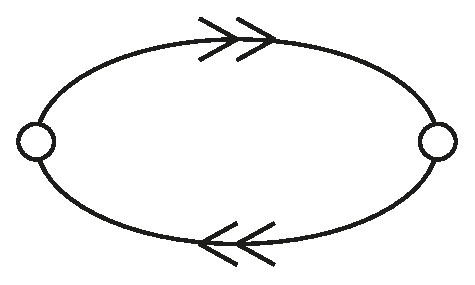
\includegraphics[scale=0.6]{1-01}
\end{figure}

The diagram has a left and right node signaling each a $U(N)$ gauge factor, so the gauge group is $SU(N)\times SU(N)$. The two arrows moving from left to right represent two different chiral fields $A_1$ and $A_2$ both in the $(\cjrep N,\rrep N)$ gauge representation, while the lower arrows are two other fields $B_1$ and $B_2$ transforming as $(\rrep N, \cjrep N)$.

Let us review briefly the structure of the action of an $\ssn \geq 1$ gauge theory; we follow \cite{wessbagger}. There is a gauge vector superfield $V$ (corresponding to an on-shell multiplet $(A_\mu,\lambda)$) with values in the algebra (that is $V = T^a V_a$ with $V_a$ in the adjoint), with an associated field-strength

\begin{equation}
	W_\alpha = - \frac{1}{4} \overline{D}_{\dot \alpha} \overline{D}^{\dot \alpha} D_\alpha V
	\label{}
\end{equation}

and the dynamics of the free vector are given by the Lagrangian

\begin{equation}
	\mathcal{L}_\mathrm{SYM} = \frac{1}{4} \int d^2 \theta \,\Tr W^\alpha W_\alpha + \operatorname{h.c.}
	\label{}
\end{equation}

In addition, one can also include chiral superfields $\Phi_I = (\varphi_I, \psi_I)$ charged under the gauge group. These will have a kinetic term

\begin{equation}
	\mathcal{L}_\Phi = \int d^4\theta\, \Phi^\dagger_I e^{gV} \Phi_I
	\label{}
\end{equation}

which is a correction of the canonical $\int d^4 \theta \, \Phi^\dagger_I \Phi_I$ to implement gauge invariance. $g$ is the gauge coupling; note this means that one should really introduce separate gauge fields for each simple factor in the gauge group, as each one will have an independent coupling. Finally, one is free to add an interaction superpotential for the chiral fields:

\begin{equation}
	\mathcal{L}_\mathrm{int} = \int d^2 \theta\, W(\Phi) + \operatorname{h.c.}
	\label{}
\end{equation}

provided $W$ is a gauge invariant combination of the $\Phi_I$.

\subsection{Renormalization and supersymmetric beta functions}

In the study of D3-brane quiver theories we will need to identify their conformal manifolds as defined in \ref{sec:scft}, or less ambitiously just its dimension. This is the number of marginal directions, deformations of the theory that preserve its superconformal invariance. In general we will have a space of parameters $(g_1, g_2, \ldots, g_\chi, \lambda_1, \ldots, \lambda_k)$ including gauge and superpotential couplings, and the conformal manifold will be the submanifolds of values of these couplings for which $\beta_{g_1} = \ldots = \beta_{g_\chi} = \beta_{\lambda_1} = \ldots = \beta_{\lambda_k} = 0$.

Thankfully, the renormalization structure of supersymmetric theories is in general vastly simplified with respect to the general case. In the case of $\ssn \geq 1$ supersymmetry, there is a remarkably simple formula for the gauge beta functions, connecting them to the anomalous dimensions of the fields:

\begin{equation}
	\beta(g_a) = - \frac{g_a^3}{16\pi^2} \frac{3 T[\mathrm{Adj}] - \sum_i T[R_i] (1- 2\gamma_i) }{1-Ng_a^2 / 8\pi^2 }\,.
	\label{nszv}
\end{equation}

$T[R]$ is the Dynkin index of the representation $R$ of the gauge group. The sum is over the chiral fields charged under the gauge group, and their representations and anomalous dimensions $R_i$, $\gamma_i$. This is known as the Novikov-Shifman-Vainshtein-Zakharov (NSVZ) $\beta$ function, and is known to be correct to all orders in perturbation theory\cite{Carlino:1999tc}. A further simplifying step will be possible because in addition to supersymmetry the theory has superconformal invariance, as the anomalous dimension $\gamma = \Delta - 1$ will be connected to the R-charge at conformal points according to \eqref{deltarcharge}.

For what concerns instead the $\beta$ functions for superpotential couplings, it is easy to see the scale-invariance of the action corresponds to an exact R-charge of $2$ for the superpotential. Therefore the vanishing of these $\beta$ functions is equivalent to imposing the sum of R-charges of the entering chiral fields is $2$.



We now are ready to begin our investigation of the following specific chain of theories:

\begin{center}
\begin{tabular}{|c | c | c|}
	\hline
	Theory & $\ssn$ & Quiver diagram  \\
	\hline \hline
	$\ssn = 4$ Super-Yang-Mills & $4$ & 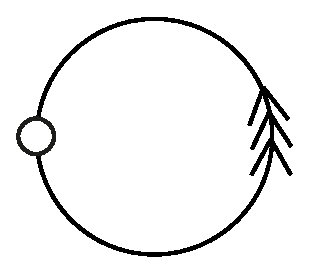
\includegraphics[scale=0.2]{4-01}\\ \hline 
	\multicolumn{3}{c}{ $\downarrow$ $\mathbb{Z}_2$ orbifold} \\ \hline
	$\mathbb{C}^3/\mathbb{Z}_2$ & $2$ & 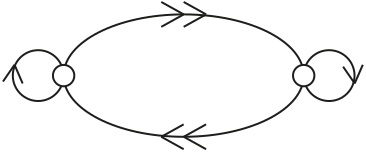
\includegraphics[scale=0.2]{2-01} \\ \hline
	\multicolumn{3}{c}{ $\downarrow$ mass deformation} \\ \hline
	Klebanov-Witten & $1$ & 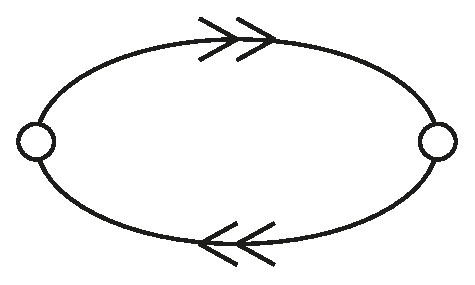
\includegraphics[scale=0.2]{1-01}\\ \hline
	\multicolumn{3}{c}{ $\downarrow$ $\mathbb{Z}_2$ orbifold} \\ \hline
	$Y^{2,0}$ & $1$ & 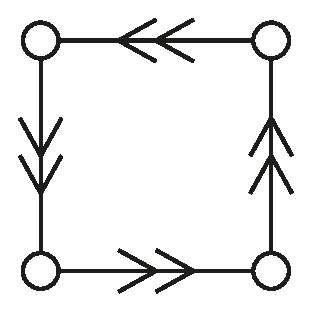
\includegraphics[scale=0.2]{3-01}\\ \hline
\end{tabular}
\end{center}

The transformations turning each theory into the next will be explained progressively.

\section{Brane stack in $\mathbb{C}^3$ and $\mathcal{N}=4$ super-Yang-Mills} \label{SYM4}

If $X_6 = \mathbb{C}^3$, the branes are invariant under half of the $16 \times 2 = 32$ IIB supercharges. This implies $\mathcal{N}=4$ for the field theory. Moreover, the theory features gluons as the massless spin-1 modes for the sector of strings stretching between brane $i$ and brane $j$ so that the gauge group is $U(N)$, as seen in \ref{sec:branestacks}. The information that the theory is a $U(N)$ gauge theory and is maximally supersymmetric is enough to uniquely fix it. Actually, since our main interest is in the IR limit, the $U(1)$ gauge factor decouples as we have explained in general, and the group is reduced to $SU(N)$.

In $\mathcal{N}=1$ language (which we employ even though the model has $\mathcal{N}=4$) the theory describes the dynamics of an $U(N)$ gauge vector supermultiplet $V_\mu$ and three complex chiral superfields $(X^a)_{i\dot j}$, $a=1,2,3$ in the adjoint of the gauge group (we will frequently omit gauge indices). These are nothing else than the parametrization of the D3-branes' position in $\mathbb{C}^3$ and therefore transform in the fundamental of $SU(3)$. The superpotential is the only one allowed by gauge and $SU(3)$ invariance,

\begin{equation} W(X) = g \epsilon_{abc} \Tr ( X^a X^b X^c) \label{sym4potential}\,;
\end{equation}

note the coupling $g$ is also the coupling of the gauge group, not an indipendent parameter. Since the theory has a single $SU(N)$ factor in the gauge group, and three fields in the adjoint (which is trivially a bifundamental with the same node at the two ends), the quiver diagram is rather simple:

\tikzset{% arrow close to the source: the 0.2 determines where the arrow is drawn
  ->-/.style={decoration={markings, mark=at position 0.5 with {\arrow{stealth}}},
              postaction={decorate}},
}

\begin{figure}[H]
	\centering
%\begin{tikzpicture}[every node/.style={circle,draw},thick,scale=1.5]
%  \node(NL) at (0,0){};
%  \draw[->-](NL.north) to [loop above, min distance=20mm, in=-45, out=45, looseness=8]	(NL.south);
%  \draw[->-](NL.north) to [loop above, min distance=24mm, in=-45, out=45, looseness=8]	(NL.south);
%  \draw[->-](NL.north) to [loop above, min distance=28mm, in=-45, out=45, looseness=8]	(NL.south);
%\end{tikzpicture}
	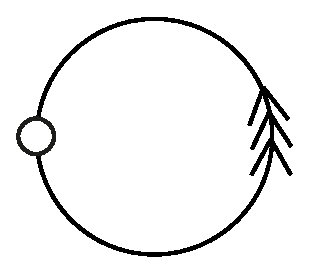
\includegraphics[scale=0.5]{4-01}
\end{figure}


Note that the obvious global symmetries, the $U(1)$ R-charge for $\ssn = 1$ and the $SU(3)$ flavour symmetry acting on the $X^a$ are actually just a subgroup of a $SU(4)$ R-symmetry group for the hidden $\ssn = 4$ supersymmetry. To make this manifest, split the $\ssn=1$ superfields as $V \rightarrow (A_\mu,\lambda)$ and $X^a \rightarrow (\phi^a,\psi^a)$, and regroup the fields as

\begin{align}
	\lambda^\alpha := (\lambda,\psi^1,\psi^2,\psi^3)\,,\quad \phi^i =: \varphi^i + i \varphi^{i+3}\,,
	\label{}
\end{align}

then $(A_\mu,\lambda^\alpha,\varphi^i)$ form an $\ssn=4$ vector supermultiplet, the components transforming respectively as $\mathbf{1}$, $\mathbf{4}$, $\mathbf{6}$ under R $SU(4)$, and in the adjoint of gauge $SU(N)$.

\subsection{Marginal deformations}

$\ssn = 4$ (maximal) supersymmetry is extremely constraining, and indeed a non-renormalization theorem (first proven nonperturbatively in \cite{seibergnr}) states the theory is exactly finite. No divergences means the $\beta$ function (one for the only gauge coupling) vanishes identically, and the theory is always superconformal. Indeed, there is a set of additional 16 supercharges beyond the standard ones. These do \emph{not} however find a direct correspondence as supersymmetries of the D3-brane system, but only of the ``near-horizon'' ($\alpha' \rightarrow 0$) geometry of the brane stack.

However, one can also discuss the vanishing of the beta function in $\ssn = 1$ language as a trivial example. We note $SU(3)$ flavour symmetry imposes that the R-charges and anomalous dimensions of the three chiral fields are equal. Then, for the superpotential to be scale invariant we need $R_W$ to be $2$, so

\begin{equation}
	R_W = 2 = R + R + R \Rightarrow R = \frac{2}{3} \Rightarrow \gamma = 0\,,
	\label{}
\end{equation}

where \eqref{deltarcharge} was used; thus, the chiral fields have canonical dimension. Then the NVSZ beta function for the gauge coupling reads

\begin{equation}
	\beta_\tau \propto 3 N - 3 N (1-2\gamma) = 3N-3N = 0\,.
\end{equation}

So, this vanishes identically, for all values of the coupling $\tau$. Thus the conformal manifold of such a theory is minimal: there is a single marginal deformation corresponding to changing $\tau$, and the theory is a SCFT for every value of this unique parameter.

\subsection{Moduli space}

One could wonder instead about the moduli space $\mathcal{M}$ of the theory. This is the space of inequivalent vacua; classically, one plugs uniform vacuum expectation values $X^a$ for the chiral fields into the action to get an effective potential:

\begin{equation}
	\mathcal{V}(X^a) = \pder{W^\dagger}{X^\dagger_a} \pder{W}{X^a} =: F^{a\dagger} F_a\,,
	\label{}
\end{equation}

which is then minimized. Since $\mathcal{V} \geq 0$ and it equals zero at the special point $X^a = 0$, its minima will coincide with its zeroes, which occurr when all of the $F^a$ vanish:

\begin{equation}
	F_a := \pder{W}{X^a}\,
	\label{fflatness}
\end{equation}

$F_a$ is known as an F-term and the conditition \eqref{fflatness} is known as an F-flatness condition.

The moduli space of SYM4 is then very easy to describe. The F-term conditions simply read:

\begin{equation}
	\pder{W}{X^a} \propto \varepsilon_{abc} X^b X^c = 0\,,
	\label{}
\end{equation}

so that the space of solution is given by (VEVs of) $X^a$ that commute with eachother as $N\times N$ matrices. Therefore, they can be simultaneously diagonalized by a gauge transformation, and the $3N$ eigenvalues $x^a_I$, $I=1,\ldots,N$ are completely free. In fact, these coincide directly with the coordinates of the $N$ D3-brane on $\mathbb{C}^3$. The moduli space is $\mathbb{C}^{3N}$, or to be precise, taking into account brane indistinguishability (i.e., the residual permutation gauge symmetry after diagonalization of the $X^a$),

\begin{equation}
	\mathcal{M} = \operatorname{Sym}^N \mathbb{C}^3\,.
	\label{}
\end{equation}

In fact, this structure will always be present in D3-brane theories. Moduli space will always include a $\mmes \subset \mathcal{M}$ describing the motion of the D-branes on $X_6$, and it will be true in general that $\mmes = \operatorname{Sym}^N X_6$. However, $\mmes$ will not comprise the totality of moduli space and in more complex theories additional directions to $\mathcal{M}$ will arise.

\section{$\mathbb{C}^3/\mathbb{Z}_2$ orbifold}

We now move to a less trivial case by performing an orbifold of the background. Essentially, we act on $\mathbb{C}^3$ as such

\begin{equation}
	(z^1, z^2, z^3) \mapsto (-z^1, -z^2, z^3)
	\label{}
\end{equation}

and quotient under this $\mathbb{Z}_2$ group. This yields a Calabi-Yau manifold with a conical singularity in $z^1 = z^2 =0$. Equivalently, if the background is presented in polar coordinates as $\mathbb{R}_+ \times \mathbb{S}^5$, the orbifold produces $\mathbb{R}_+ \times (\mathbb{S}^5 / \mathbb{Z}_2)$. Our interested is then for the worldvolume theory of $N$ D3-branes placed in this singular background.

To investigate this, we consider $\tilde N = 2N$ D3-branes on $\mathbb{C}^3$, producing SYM4 as seen in the previous section, then we act on the $A_\mu$ and $X^a$ fields with the $\mathbb{Z}_2$ action and select the subset of invariant fields - these will be the degrees of freedom of the orbifold theory.

We need to specify an action of $\mathbb{Z}_2$ on the gauge indices. The following choice is convenient: act on an object in the fundamental $\mathbf{\tilde N} = \mathbf{N} \oplus \mathbf{N}$ as $1$ on the first factor and $-1$ on the second. This means, for example, that having decomposed $A_\mu$ in subrepresentations its transformation under $\mathbb{Z}_2$ is

\begin{equation}
	A_\mu = \begin{pmatrix}
		A^{0,0} & A^{1,0} \\
		A^{0,1} & A^{1,1}
	\end{pmatrix} \mapsto \begin{pmatrix}
		A^{0,0} & -A^{1,0} \\
		-A^{0,1} & A^{1,1}
	\end{pmatrix}\,,
\end{equation}

where $A^{i,j}$ are $N\times N$ matrices. We see the surviving gauge fields are $A^{0,0}$ and $A^{1,1}$, adjoint for the $U(N) \times U(N)$ subgroup of $U(2\tilde N)$. The new gauge group is therefore $U(N) \times U(N)$.

The same holds for $X^3$, which becomes $\Phi := (X^3)^{0,0}$ and $\tilde \Phi := (X^3)^{1,1}$, two chiral fields each in the adjoint of one of the $U(N)$ factors.

For $X^1$, $X^2$ instead one has to take into account both the action on the gauge indices and the direct action on the $\mathbb{C}^3$ geometry. With $i=1,2$, one has

\begin{equation}
	X^i = \begin{pmatrix} 
			(X^i)^{0,0} & (X^i)^{1,0} \\
			(X^i)^{1,0} & (X^i)^{1,1} 
		\end{pmatrix}\mapsto \begin{pmatrix} 
			-(X^i)^{0,0} & (X^i)^{1,0} \\
			(X^i)^{1,0} & -(X^i)^{1,1} 
		\end{pmatrix}\,,
\end{equation}

and one ends up with two pairs of chiral fields in bifundamentals, $A^i := (X^i)^{0,1}$, $B^i := (X^i)^{1,0}$, in representations $(\rrep N, \cjrep N)$ and $(\cjrep N, \rrep N)$ of $U(N)\times U(N)$ respectively. The structure of the theory can be more elegantly presented in a quiver diagram:

\begin{figure}[H]
	\centering
%\begin{tikzpicture}[every node/.style={circle,draw},thick,scale=1.5]
%  \node(NL) at (0,0){};
%  \node(NR) at (2,0){};
%  \draw[->-](NL.north) to [bend left=60]	(NR.north);
%  \draw[->-](NL.north) to [bend left=90]	(NR.north);
%  \draw[->-](NR.south) to [bend left=60]	(NL.south);
%  \draw[->-](NR.south) to [bend left=90]	(NL.south);
%  \draw[->-] (NL.south west) to [loop left, min distance=5mm, in=120, out=230, looseness=10] (NL.north west);
%  \draw[->-] (NR.south east) to [loop left, min distance=5mm, in=60, out=300, looseness=10] (NR.north east);
%\end{tikzpicture}
	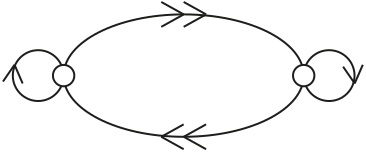
\includegraphics[scale=0.5]{2-01}
\end{figure}

The superpotential is just given by restriction of the SYM4 potential \eqref{sym4potential} to the surviving fields; after some algebra

\begin{equation}
	W = \mu \left( \Tr \Phi (A_1 B_1 + A_2 B_2 ) + \Tr \tilde\Phi (B_1 A_1 + B_2 A_2) \right)
	\label{}
\end{equation}

It is clear at this point that, given the introduction of an asymmetry between $X^3$ and $X^{1,2}$, the $\ssn = 4$ R-symmetry $SU(4)$ is broken and so is maximal supersymmetry. The orbifold theory has indeed $\mathcal{N}=2$ supersymmetry\cite{Douglas}.

%\cmmnt{--Tutto ci\`o che c'\`e qua sotto dove si trova?--}
%
%This theory, moreover, is also superconformal at some points. The form of the potential is again fixed (there are no possible deformation consistent with the remaining symmetries) except for the overall constant $\mu$; therefore a set of parameters for the theory is given by the three couplings $(\tau_1,\tau_2,\mu)$, where we have accounted for the fact that the two gauge factors can flow independently under the renormalization group. Then, the vanishing of the $\beta_\mu$ function for the $\mu$ coupling is equivalent the R-charge of the superpotential being $2$, so that
%
%\begin{equation}
%	R_\Phi + R_A + R_B = 2\,,\quad R_{\tilde\Phi} + R_A + R_B = 2
%	\label{}
%\end{equation}
%
%which, employing $\frac{3}{2}R = 1+\gamma$ for chiral fields at a superconformal point, is equivalent to
%
%\begin{equation}
%	\gamma_\Phi + \gamma_A + \gamma_B = 0 = \gamma_{\tilde \Phi} + \gamma_A + \gamma_B\,.
%	\label{}
%\end{equation}
%
%We combine this with the vanishing of the two gauge $\beta$ functions. Using the NSVZ formula for the left node we get
%
%\begin{equation}
%	\beta \propto 3N-N(1-2\gamma_\Phi) - 2 \frac{N}{2} ( 1-2\gamma_A) - 2 \frac{N}{2} (1- 2\gamma_B) = 2 ( \gamma_\Phi + \gamma_A + \gamma_B) = 0\,,
%	\label{}
%\end{equation}
%
%and identically for the other gauge node, replacing $\Phi$ with $\tilde\Phi$. Therefore the conformal conditions are not all independent: only two independent conditions determine the conformal manifold. Since we have a three parameter space $(\tau_1, \tau_2, \mu)$, the locus of conformal points will be 1-dimensional. At a generic point $(\tau_1,\tau_2,\mu)$ in parameter space the theory will not be superconformal; however it should flow in the IR towards a point on the conformal curve.
%
%Directions along the conformal manifolds are marginal deformations of the theory, as seen before. In this case, one marginal deformation will be present.
%
%\cmmnt{Moduli space? Forse $b_3(Y) = 0$?}

We will not concentrate on the details of this $\mathbb{C}^3/\mathbb{Z}_2$ theory; we use it as a stepping stone from SYM4 to the Klebanov-Witten theory, which we will introduce in the next section as a deformation of the orbifold theory.

\section{The conifold and the Klebanov-Witten model} \label{sec:KW}

In \cite{KW_SCFT} the case of $X_6$ being the conifold was studied. The conifold is a specific Calabi-Yau 3-cone defined for example as the following variety in $\mathbb{C}^4$:

\begin{equation}
	z_1^2 + z_2^2 + z_3^2 + z_4^2 = 0\,,
\end{equation}

with the K\"ahler structure inherited from the standard one on $\mathbb{C}^4$, or, after a simple change of variables:

\begin{equation}
	u v - xy = 0\,.
	\label{conifoldeq}
\end{equation}

The base can be found by quotienting by dilations $z_i \rightarrow \lambda z_i$ (with $\lambda \in \mathbb{R}_+$) and turns out to be the homogeneous space $SO(4)/U(1) = SU(2)\times SU(2) / U(1)$, where the $U(1)$ is a diagonal subgroup generated by, say, $T^3_L + T^3_R$. Topologically, this is $\mathbb{S}^2 \times \mathbb{S}^3$. We will therefore have $SU(2)\times SU(2)$ as part of the isometry group of both $Y_5$ and $X_6$, and thus will also appear as a global symmetry of the wordvolume theory. An equivalent description of the topology of the conifold is as a $U(1)$ bundle over $\mathbb{C}P^1 \times \mathbb{C}P^1 \cong \mathbb{S}^2 \times \mathbb{S}^2$; in these terms the metric on this cone is

\begin{gather}
	ds^2_6 = dr^2 + r^2 ds^2_5 \nonumber\\
	ds^2_5 = \frac{1}{9} (d\psi + \cos\theta_1 d\phi_1 + \cos\theta_2 d\phi_2)^2 + \frac{1}{6} (d\Omega_1^2 + d\Omega_2^2)\label{conifoldmetric}
\end{gather}

where $\Omega_i^2 = d\theta_i^2 + \sin\theta_i^2 d\phi_i^2$ is the metric on the $\mathbb{C}P^1_i$, and $\psi$ is the fibral coordinate with period $4\pi$.

The corresponding field theory (which we will call the Klebanov-Witten model), however, can also be found by applying a particular modification to the orbifold theory of the previous section\cite{KW_SCFT}. Let us derive the form of this SCFT in this way, and then show how the above geometry reappears from the field theory side. The modification is the addition of a relevant term to the Lagrangian, a mass for the $\Phi$, $\tilde\Phi$ adjoint fields

\begin{equation}
	\mathcal{M} = \frac{M}{2} \left( \Tr \Phi^2 - \Tr \tilde\Phi^2 \right)\,,
	\label{massterm}
\end{equation}

thus providing a possible UV completion for the $\mathbb{C}^3/\mathbb{Z}_2$ theory. These fields are then eliminated using the resulting classical equations of motion. For example,

\begin{equation}
	\pder{(\mathcal{M} + W)}{\Phi} = 0 \Rightarrow \Phi = - \frac{\mu}{M} \left( A_1 B_1 + A_2 B_2 \right)
	\label{}
\end{equation}

and analogously for $\tilde \Phi$. Finally, these are substituted back into the action, reducing the chiral fields to just $A_i$ and $B_i$ and the superpotential to

\begin{equation}
	W = \frac{\lambda}{2} \epsilon^{ij} \epsilon^{kl} \Tr \left( A_i B_k A_j B_l \right)
	\label{kwpotential}
\end{equation}

having defined $\lambda := \frac{\mu^2}{2M}$. More formally, it is argued that after the introduction of the relevant term \eqref{massterm} the $\mathbb{C}^3/\mathbb{Z}_2$ theory flows in the IR to the Klebanov-Witten model.

Therefore, the worldvolume gauge theory is a $U(N)\times U(N)$ field theory featuring two chiral doublets $A_i$, $B_j$ with $i,j = 1,2$ transforming in opposite bifundamentals, that is $A_i$ in $(N,\bar N)$ and $B_j$ in $(\bar N, N)$. The quiver diagram is simpler:

\begin{figure}[H]
	\centering
%\begin{tikzpicture}[every node/.style={circle,draw},thick,scale=1.5]
%  \node(NL) at (0,0){};
%  \node(NR) at (2,0){};
%  \draw[->-](NL.north) to [bend left=60]	(NR.north);
%  \draw[->-](NL.north) to [bend left=90]	(NR.north);
%  \draw[->-](NR.south) to [bend left=60]	(NL.south);
%  \draw[->-](NR.south) to [bend left=90]	(NL.south);
%\end{tikzpicture}
	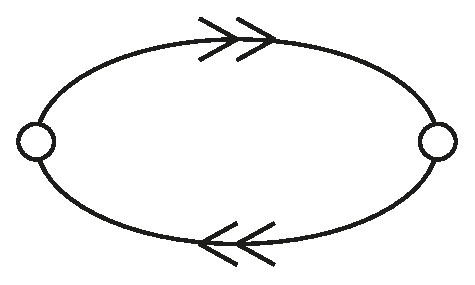
\includegraphics[scale=0.5]{1-01}
\end{figure}

The $i$ and $j$ indices, instead, are acted upon respectively by the global left and right $SU(2)$ symmetries. From the form of the superpotential and these symmetries, furthermore, it is possible to deduce the R-charges of $A_i$ and $B_i$ are $1/2$, implying a dimension of $\Delta = 3/4$ when the theory is conformal. A non-canonical scaling dimension is a symptom that the CFT will always be strongly-coupled.

It is also clear the supersymmetry has been broken further to $\ssn = 1$, since \eqref{massterm} is not $\ssn = 2$ invariant ($\Phi$, $\tilde \Phi$ were actually combined with $A_i$, $B_i$ into $\ssn = 2$ hypermultiplets in the orbifold theory). The case at hand is thus a four-dimensional strongly-coupled field theory with minimal supersymmetry.

\subsection{Marginal deformations}

The Klebanov-Witten theory will not be in general superconformal; it will flow through renormalization in the IR to a conformal submanifold in the space of couplings $(\lambda,\tau_1,\tau_2)$, the locus where the $\beta$ functions for these three couplings vanish. It turns out these three conditions are all equivalent. In particular, requiring either $\beta_{\tau_1} = 0$ or $\beta_{\tau_2} = 0$ and making use of the NSZV \eqref{nszv} this unique condition is equivalent to

\begin{equation}
	3 T[\mathrm{Adj}] - \sum_i T[R_i] ( 1- 2\gamma_i) = 0\,.
	\label{}
\end{equation}

When evaluating this, care should be taken with the fact that $A_i$ and $B_j$ have a $U(N)_2$ index which is uncharged under $U(N)_1$ and must be summed over. Noting $\gamma_{A_1} = \gamma_{A_2}$ and $\gamma_{B_1} = \gamma_{B_2}$ because of the global flavour $SU(2)\times SU(2)$ symmetry, this gives

\begin{equation}
	\gamma_A + \gamma_B + \frac{1}{2} = 0\,.
	\label{}
\end{equation}

Being $\gamma_{A,B}$ functions of the couplings, this equation defines a critical 2-surface in parameter space. Switching to R-charges, this means

\begin{equation}
	R_A + R_B = 1\,,
	\label{}
\end{equation}

but this is also the equation for the vanishing of the $\beta$ function for the superpotential coupling $\lambda$, since $R_W = 2$ is just

\begin{equation}
	R_A + R_B + R_A + R_B = 2\,.
	\label{}
\end{equation}

Thus, since the three conditions are equivalent, the final conformal manifold is the locus of a single equation in three variables $(\lambda,\tau_1,\tau_2)$ and is then two-dimensional. Therefore there will be two marginal deformations of the theory.

\subsection{Global $U(1)$} \label{sec:kwuone}

Let us comment briefly on the whereabouts of the abelian gauge factors of $U(N) \times U(N)$ under RG flow towards the infrared. Denoting as $T^1$ and $T^2$ the generators of the two trace $U(1)$ of the left and right nodes, it is clear $T^1+T^2$ is the overall completely decoupled $U(1)_\text{trace}$ that we can safely ignore. The only remaining abelian factor is generated by $B = T^1 - T^2$. This symmetry is non-anomalous; since it is an abelian gauge interaction with massless charged matter, under RG flow towards the infrared its coupling vanishes and thus freezes into a rigid $U(1)_\text{baryonic}$ in the IR. We call this charge, corresponding to the symmetry

\begin{equation}
	A_i \rightarrow e^{i\theta} A_i\,,\quad B_i \rightarrow e^{-i\theta} B_i
	\label{}
\end{equation}

a baryon number. This quantum number will become important in classifying gauge invariant operators.\cmmnt{???}

\subsection{Moduli space}

Position in moduli space $\mathcal{M}$ should be parametrized by the expectation values of gauge-invariant operator (hadrons). This should be obtained, as it was sketched for SYM4, by considering the locus of minima of the effective potential $\mathcal{V}$ in the space of VEVs of the chiral fields, and then quotienting by complexified gauge transformations. Taking for the moment a general $\ssn=1$ theory with gauge generators $T^a$ and chiral fields $\phi^i$, the effective potential can be found to be

\begin{equation}
	\mathcal{V}(\phi) \;=\; \frac{g_a^2}{2} (\phi^\dagger T^a \phi)^2 + \pder{W^\dagger}{\phi^\dagger_i} \pder{W}{\phi^i} \; =:\; \frac{g_a^2}{2} (D^a)^2 + F^\dagger_i F^i
	\label{}
\end{equation}

We have defined the F-terms and the D-terms:

\begin{align}
	F^i &= \pder{W}{\phi^i}\,,\label{ftermdef}\\
	D^a &= \sum_i \phi_i^\dagger T^a \phi_i\,.\label{dtermdef}
\end{align}

Again, $\mathcal{V}$ will be minimum when $\mathcal{V}=0$, thus when the F-term and D-term vanish, conditions we will call F-flatness and D-flatness. The space of simultaneous solutions to $F^i = D^a = 0$, quotiented by gauge transformations, will be moduli space $\mathcal{M}$.

Specializing to the Klebanov-Witten model, $D^a = 0$ will hold only with $a$ spanning over generators of $SU(N) \times SU(N)$, not involving the abelian factors $U(1)_1\times U(1)_2 = U(1)_\text{trace} \times U(1)_\text{baryon}$, since according to our discussion in section \ref{sec:kwuone} these do not survive as gauge symmetries in the IR. The D-term of $U(1)_\text{trace}$ has no significance, since this is completely decoupled and vanishes identically. The baryon D-term instead gets relaxed

\begin{equation}
	D^{U(1)_\text{baryon}} = \xi
	\label{}
\end{equation}

where $\xi$ is an arbitrary parameter. Actually, $\xi$ is a modulus, parametrizing a direction in $\mathcal{M}$ itself. Indeed, it is the only additional direction in $\mathcal{M}$ to those along $\mmes$, which is a strict subset of the KW moduli space. Let us determine $\mathcal{M}$, identify $\mmes$ and verify these claims. The vanishing of the F-terms \eqref{ftermdef} and D-terms \eqref{dtermdef}, specialized to the particular case, are

\begin{equation}
	\epsilon^{ij} A_i B_a A_j = \epsilon^{ij} B_i A_a B_j = 0
	\label{}
\end{equation}

\begin{equation}
	A_i A_i^\dagger - B_i B_i^\dagger = A^\dagger_i A_i - B^\dagger_i B_i = \xi \mathbbm{1}
	\label{}
\end{equation}

the equation have to be understood to hold for VEVs. Note the first and second D-term condition are respectively from the left and right gauge group. 

Consider the subset of $\mathcal{M}$ with $\xi = 0$; our claim is this is precisely $\mmes$. To reinterpret the F-flatness condition, we introduce the four matrices $\Phi_{ij} = A_i B_j$ and note

\begin{align}
	\left[ \Phi_{ij} , \Phi_{jk} \right] = 0\\
	\Phi_{11} \Phi_{22} = \Phi_{21}\Phi_{12}
	\label{}
\end{align}

which can be immediately checked to follow from the vanishing of the F-term. Since these commute, they can be simultaneously diagonalized and their $N$ eigenvalues (one for each brane) satisfy the conifold's equation \eqref{conifoldeq}:

\begin{equation}
	\phi^I_{11} \phi^I_{22} = \phi_{21}^I \phi_{12}^I
	\label{}
\end{equation}

so these quite literally parametrize the motion of the $N$ D3-branes on the background cone. These actually determine the VEVs of mesonic operators, mesons\footnote{The meson/baryon terminology is meant to be a direct generalization of the concept of QCD hadrons. A QCD meson is to a first approximation built from two quarks as a symmetric product $\ket{M} \sim \delta^i_{\,j} \ket{q^i \overline q_j} + \mathcal O (gluons)$, while a baryon is $\ket{B} \sim \epsilon_{ijk} \ket{q^i q^j q^k}$. In general, $SU(N)$-singlets can be built by contracting gauge indices either with the symmetrical $\delta^i_j$ or the antisymmetric $\epsilon_{a_1 \ldots a_N}$.} being generated by prototipical trace operators:

\begin{equation}
	M_{(ab\ldots),(ij\ldots)} =	\Tr\left( (A_a B_i)(A_b B_j)\cdots \right)\,.
	\label{}
\end{equation}

This justifies the terminology of ``mesonic moduli space'' for the submanifold $\mmes$ of $\mathcal{M}$ they describe.

Note mesons are built by tracing over closed loops in the quiver diagram to make a gauge-invariant operator. All of these operators are actually expressable as products of $\Phi$ matrices, and as it was shown, only $3$ out of $4$ of those are independent. In the end, there are (accounting for gauge indices) $3N$ independent mesons whose VEVs parametrize mesonic moduli space, coincident with the $\operatorname{Sym}^N C$, where $C$ is the conifold.

Operators of non-zero baryon number can also be constructed by using the antisymmetric invariant gauge tensor $\epsilon^{a_1\ldots a_N}$, as such:

\begin{equation}
	\mathcal{B}^A_{[k]} = \epsilon^{a_1\ldots a_N} \epsilon_{b_1\ldots b_n} (A_1)_{a_1}^{b_1} \ldots (A_1)^{a_k}_{b_k} (A_2)^{a_{k+1}}_{b_{k+1}} \ldots (A_2)^{b_N}_{a_N}
	\label{}
\end{equation}

where we have displayed gauge indices on the $A$ fields. There are only $N+1$ different assignment for the $SU(2)$ indices because of antisymmetry, so that there are $N+1$ fundamental baryons of the form of $\mathcal{B}^A$. The same could be done by swapping the two gauge groups and using $B$ fields, to get additional $N+1$ $\mathcal{B}^B$ baryons. These all have baryon number $N$ under $U(1)_\text{baryonic}$ while mesons have baryon number $0$.

All gauge-invariant operators in the theory are built out of these fundamental mesons, fundamental baryons, and their respective antiparticles (made out of the conjugate fields $A^\dagger$, $B^\dagger$. However, as we have anticipated, we only expect $g-1 = 1$ baryonic VEV to be independent. This VEV will be associated with the resolution of the cone singularity into a $\mathbb{CP}^1 \cong \mathbb{S}^2$, and will essentially coincide with $\xi$. To see an example of this deformation of the background geometry, let us set $\xi$ to a constant nonzero value. Then hypothesizing for simplicity that the $A_1, A_2, B_1, B_2$ matrices commute, applying F-term conditions we get that each set of eigenvalues satisfies

\begin{equation}
	a_1/a_2 = b_1/b_2
	\label{}
\end{equation}

So that $a_i$ and $b_i$ are proportional vectors of $\mathbb{C}^2$, therefore

\begin{equation}
	a_i = a e^{i\theta_A} n_i, \quad \quad b e^{i\theta_B} n_i
	\label{}
\end{equation}

where $a,b$ are real and $n_i$ belongs to a $\mathbb{CP}^1$. The phases are cancelled by modding gauge invariance, and $a$ and $b$ then are involved in the D-term:

\begin{equation}
	a^2 - b^2 = \xi
	\label{}
\end{equation}

so that essentially our mesonic VEVs are composed of $N$ copies of one non-compact radial coordinate (say, $a$) and a point on $\mathbb{CP}^1$. This means the conical singularity has disappeared to be replaced by a two-cycle on which the branes can move.

A more thorough investigation of the geometry probed by these mesonic directions when $\xi$ has a non-zero value would show the D3-branes are moving on the geometry of the resolved conifold, the metric\cite{PandoZayas}

\begin{equation}
	ds_6^2 = \kappa^{-1} dr^2 + \frac{1}{9} \kappa r^2 (d\psi + \cos\theta_1 d\phi_1 + \cos\theta_2 d\phi_2)^2 + \frac{1}{6} r^2 d\Omega_1^2 + \frac{1}{6} (r^2 + a^2 ) d\Omega_2^2\label{resolvedconifold}
\end{equation}
\begin{equation}
	\kappa(r) = \frac{r^2 + 9a^2}{r^2 + 6a^2}
	\label{}
\end{equation}

parametrized by a modulus $a$. Turning on the $\xi$ modulus corresponds to increasing $a$ (in fact, the two are proproportional\cite{MZ}), and to the blow up of the two-sphere at $r=0$. Instead, for $a=0$ one recovers the singular conifold \eqref{conifoldmetric}.

Thus, we have uncovered the following structure for $\mathcal{M}$. It is a $(3N + 1)$-dimensional\footnote{There is an obvious dimensional mismatch in that the complex modulus $\xi$ corresponds to a real parameter $a$ in the metric. It turns out that when the real part of a modulus maps to a K\"ahler deformation, the imaginary part describes instead a modulus for the $A_4$ Ramond-Ramond form; we will explain more in chapter \ref{chap:heft}} complex manifold on which one can define the coordinate $\xi$, a baryonic modulus. The $3N$-submanifold at $\xi = 0$ is $\mmes$, which is equal to the symmetric product of $N$ copies of the conifold and is parametrized by $3N$ complex moduli, VEVs of particular combinations of mesonic operators, that can be identified with the positions of the threebranes. If instead one consider a constant but nonzero value $\xi = \xi^*$ for the baryonic modulus, the same mesonic directions define a submanifold with the structure of the symmetric product of $N$ copies of the \emph{resolved} conifold \eqref{resolvedconifold}.

The explicit form of the baryon generating this deformation in terms of the fundamental hadrons is very challenging to determine\cite{Forcella}; fortunately, we will not need it for our purposes. In any case, all of this information will be clarified in the context of holography.



\section{The $Y^{(2,0)}$ orbifold theory}\label{sec:squares}

The same construction on a $\mathbb{Z}_2$ orbifold of the conifold yields a quiver gauge theory which will be the main interest of this work. This theory has a few interesting additional features with respect to the Klebanov-Witten model while remaining relatively simple, thus being an optimal candidate for the investigation of its effective low-energy theory, which we will perform in chapter \ref{chap:y20}. It is, like the conifold theory, an $\ssn = 1$ SCFT but boasts three baryonic moduli, of which one has no clear geometric interpretation, and two anomalous $U(1)$s. We now describe this theory and extract these features.

The geometry of the base of the cone is very simply introduced in polar coordinates as 

\begin{gather}
	ds^2_6 = dr^2 + r^2 ds_5^2\nonumber\\
	ds^2_5 = \frac{1}{9} (d\psi + \cos\theta_1 d\phi_1 + \cos\theta_2 d\phi_2)^2 + \frac{1}{6} (d\Omega_1^2 + d\Omega_2^2)\label{y20conemetric}
\end{gather}

i.e., exactly the same metric in form as the conifold, but with $\psi$ now with period $2\pi$. This background and the resulting worldvolume field theory are just one entry $Y^{2,0}$ of an infinite class $Y^{p,q}$ of examples introduced in \cite{benvenutiInfinite}.

Following an identical procedure to that performed for the $\mathbb{Z}_2$ orbifold of SYM4, we can deduce the quiver diagram splits to yield four doublets of bifundamental chiral fields stretching in a square between four nodes:

\begin{figure}[H]
	\centering
%\begin{tikzpicture}[every node/.style={circle,draw},thick,scale=1.5]
%  \node(NL) at (0,0){};
%  \node(NR) at (2,0){};
%  \node(NDR) at (2,2){};
%  \node(NDL) at (0,2){};
%  \draw[->-](NL.east) to [bend right=20]	(NR.west);
%  \draw[->-](NL.east) to [bend left=20]	(NR.west);
%  \draw[->-](NR.north) to [bend right=20]	(NDR.south);
%  \draw[->-](NR.north) to [bend left=20]	(NDR.south);
%  \draw[->-](NDR.west) to [bend right=20]	(NDL.east);
%  \draw[->-](NDR.west) to [bend left=20]	(NDL.east);
%  \draw[->-](NDL.south) to [bend right=20]	(NL.north);
%  \draw[->-](NDL.south) to [bend left=20]	(NL.north);
%\end{tikzpicture}
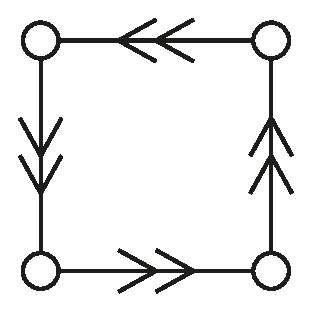
\includegraphics[scale=0.5]{3-01}
\end{figure}

so that the gauge group is $SU(N)^4$. The superpotential can be again obtained by truncation, yielding

\begin{equation}
	W = \lambda \epsilon^{ij} \epsilon^{kl} \Tr\left( A_i B_k C_j D_l \right)
	\label{squaresuperpotential}
\end{equation}

from which it is clear that the $SU(2) \times SU(2)$ isometry of the cone, corresponding to a global flavour symmetry of the field theory, must now act as

\begin{align}
	\begin{split}
		A_i \in (\rrep 2, \rrep 1)\\
		B_i \in (\rrep 1, \rrep 2)\\
		C_i \in (\rrep 2, \rrep 1)\\
		D_i \in (\rrep 1, \rrep 2)
	\end{split}
	\label{flavoursquare}
\end{align}

Note \eqref{squaresuperpotential} is also the only possible superpotential allowed by this symmetry\cite{Benvenutifourcycles}, so that the theory can also be constructed by starting with the flavour symmetry as an assumption.

\subsection{Global $U(1)$s}

The novelty in this model is the appearance of anomalous $U(1)$s. In detail, of the four gauge $U(1)$s, one (the symmetric sum) is the overall trace and decouples completely. It turns out that the three remaining abelian factors are partitioned into one non-anomalous baryonic $U(1)$ (which is inherited directly from the KW model) and two new anomalous $U(1)$s. The non-anomalous baryon number acts on $A_i$, $C_i$ with charge $+1$ and $B_i$, $D_i$ with charge $-1$, a fact obvious from orbifold of the KW baryon number. The action of the two anomalous $U(1)$s has an arbitrariness as they can obviously be shifted by the trace or non-anomalous charge; an example of charge assignments could be

\begin{center}
	\begin{tabular}[]{c|c}
		charges of $A$, $B$, $C$, $D$ & $U(1)$ \\ \hline \hline
		$(+1,+1,+1,+1)$ & Trace (decoupled) \\  \hline
		$(+1,-1,+1,-1)$ & Non-anomalous baryon number \\ 
		$(+1,+1,-1,-1)$ & Anomalous \\ 
		$(+1,+1,+1,-1)$ & Anomalous  
	\end{tabular}
\end{center}

We have already commented on how the non-anomalous abelian factor becomes a rigid global symmetry flowing down to the IR. However, the anomaly of the other two abelian gauge symmetries is worrying as it would make the theory inconsistent. Actually, it turns out these anomalies are cancelled at the level of the supergravity background by the contribution of axionic fields charged under the anomalous $U(1)$s; in particular the $Y^{2,0}$ cone has a 2-cycle $S$ and a 4-cycle $Q$ such that the integrals

\begin{equation}
	\phi_1 = \int_S A_2 \quad \phi_2 = \int_Q A_4
	\label{}
\end{equation}

constitute dynamical four-dimensional fields $\phi_1(x^\mu)$, $\phi_2(x^\mu)$ which cancel the anomaly, in a form of the Green-Schwarz mechanism\footnote{This is actually expected, as string theory is quantum consistent and no configuration in it can display anomalies.}. However, these fields transform as axions under the two anomalous $U(1)$, and so break the corresponding symmetry in a St\"uckelberg mechanism, thus the corresponding photons become massive.

\subsection{Marginal deformations}

We turn to the study of marginal deformations. Again, the flavour symmetry \eqref{flavoursquare} guarantees $\gamma_{A_1} = \gamma_{A_2} = \gamma_A$ and so on. This time three of the four gauge $\beta$ functions are independent:

\begin{align}
	\begin{split}
\beta_1 = 0 \quad	& \Rightarrow  \quad	\gamma_A + \gamma_D + \frac{1}{2} = 0\,, \\
\beta_2 = 0 \quad	&  \Rightarrow	\quad	\gamma_B + \gamma_A + \frac{1}{2} = 0\,, \\
\beta_3 = 0 \quad	&  \Rightarrow	\quad	\gamma_C + \gamma_B + \frac{1}{2} = 0\,.
	\end{split}
\end{align}

In addition, $\beta_\lambda = 0$ is also not independent: at any superconformal point, $\frac{3}{2}R - 1 = \gamma$, so that the condition that $W$ be scale invariant, which is equivalent to it having R-charge $2$, becomes

\begin{equation}
	\begin{split}
	2 = R_W = R_A + R_B + R_C + R_D \\\Rightarrow \gamma_A + \gamma_B + \gamma_C + \gamma_D + 1 = 0
	\label{}
\end{split}
\end{equation}

which is indeed equivalent to the above system. Three independent equations in the five-parameter space of $(\tau_1,\tau_2,\tau_3,\tau_4,\lambda)$ define, again, a critical 2-submanifold.

\subsection{Moduli space}

Turning to the investigation of the moduli space, the F-term condition for the given superpotential read

\begin{align}
	\begin{split}
	A_\alpha B_\sigma C_\beta \epsilon^{\alpha\beta} = 0 \\
	B_\alpha C_\sigma D_\beta \epsilon^{\alpha\beta} = 0 \\
	C_\alpha D_\sigma A_\beta \epsilon^{\alpha\beta} = 0 \\
	D_\alpha A_\sigma B_\beta \epsilon^{\alpha\beta} = 0 
	\label{Ftermssquare}
\end{split}
\end{align}

For what concerns the D-terms, as in the case of the conifold we only need to consider those relative to the true gauge symmetries of the IR theory, so those for $SU(N)^4$. As we have seen in the previous section, the $U(1)$ factors either become rigid or broken. Accordingly, the abelian D-terms get relaxed into four arbitrary parameters:

\begin{equation}
	D^{U(1)_i} = \xi^i\,,\quad i = 1,2,3,4
	\label{}
\end{equation}

Combining this information, the vanishing of the D-term takes the form

\begin{align}
	\begin{split}
		A_i A^\dagger_i - B_i B^\dagger_i = \xi_1 \mathbbm{1} \\
		B_i B^\dagger_i - C_i C^\dagger_i = \xi_2 \mathbbm{1} \\
		C_i C^\dagger_i - D_i D^\dagger_i = \xi_3 \mathbbm{1} \\
		D_i D^\dagger_i - A_i A^\dagger_i = \xi_4 \mathbbm{1}
	\end{split}
	\label{Dtermssquare}
\end{align}

with the constraint $\sum_i \xi_i = 0$ (obvious by summing the four equations \eqref{Dtermssquare}, and clear since it corresponds to the trace $U(1)$). Thus $\xi^i$ include $3$ independent baryonic moduli.

We already expect that the solutions to \eqref{Ftermssquare} and \eqref{Dtermssquare} (modulo gauge symmetry) should be parametrized by $3N$ mesonic operators measuring the positions of the branes and $3$ baryonic operators associated with the $\xi^i$, and that for $\xi^i = 0$ we recover $\mmes$ corresponding to the motion of the branes on the singular $Y^{2,0}$ \eqref{y20conemetric}. Instead, for any generic non-zero constant values of $\xi^i$, the $3N$ mesons should describe the motion of $N$ D-branes on the general resolution of the cone. 

Let us investigate the geometry of the latter by taking $\xi^i$ to have generic non-zero values (with $\sum_i \xi = 0$). Again we make the simplifying assumption the eight $A, B, C, D$ matrices commute and can be simultaneously diagonalized. So, for each of the $N$ rows of corresponding eigenvalues F-flatness \eqref{Ftermssquare} reads:

\begin{align}
	a_1/a_2 = c_1/c_2 && b_1/b_2 = d_1 / d_2
	\label{}
\end{align}

thus again $a_\alpha \propto c_\alpha$ and $b_\alpha \propto d_\alpha$, so we can ``projectivize'':

\begin{align}\begin{split}
		a_\alpha = a \, e^{i\theta_A} n_\alpha \quad b_\alpha = b \, e^{i\theta_B} n_\alpha \\
		c_\alpha = c \, e^{i\theta_C} m_\alpha \quad d_\alpha = d \, e^{i\theta_D} m_\alpha 
	\end{split}\end{align}

and again the phases are modded out by gauge symmetry, and the $a, b, c, d$ real numbers are reduced to a single coordinate (schematically $r^2$) by the three independent D-flatness conditions. Therefore the resolved geometry of the singularity is now $\ess^2 \times \ess^2$, parametrized by the $(n^I_\alpha,m^I_\alpha)$ ($I=1,\ldots,N$) coordinates of the $N$ D3-branes. Thus again for generic values of the $\xi_i$ the structure of mesonic moduli space encodes the information that the branes are moving on a resolved version of $Y^{2,0}$, where the singularity has been smoothed out into an $\ess^2 \times \ess^2$.

More specifically, there are actually two moduli describing deformations of the background cone\cite{Benvenutifourcycles}. One considers the general Calabi-Yau deformation of $Y^{2,0}$, which is given by\cite{PandoZayasy20}

\begin{equation}
	\begin{split}
	ds^2 = \kappa^{-1}(r) dr^2 + \frac{1}{9} \kappa(r) r^2 \left( d\psi + \cos\theta_1 d\varphi_1 + \cos\theta_2 d\varphi_2 \right)^2 \\
	+ \frac{1}{6} r^2 d\Omega_1^2 + \frac{1}{6}(r^2 + a^2) d\Omega_2^2\,,
	\label{genCYy20cones}
\end{split}
\end{equation}

\begin{equation}
	\kappa(r) = \frac{1 + \frac{9a^2}{r^2} - \frac{b^6}{r^6}}{1 + \frac{6a^2}{r^2}}\,.
	\label{}
\end{equation}

It can be seen that the singular $Y^{2,0}$ cone is obtained as the two moduli $a$, $b$ vanish. Turning on the $b$ modulus the volume of the four-dimensional base $\ess^2\times \ess^2$ is increased (one speaks of a blow up) and the singular tip\footnote{This does not actually lie at $r=0$ because of the way the $r$ coordinate is defined, rather it corresponds to $\kappa(r) = 0$; we will clarify this in our study of the $Y^{2,0}$ resolved geometry in chapter \ref{chap:y20}} of the cone is resolved as an $\ess^2 \times \ess^2$. The modulus $a$ instead controls the relative volume of the two spheres. Therefore there are also specific values of $(a,b)$ (or, equivalently, of the $\xi_i$) such that we have a ``partial'' resolution where only one of the spheres is blown up and branes move on an $\ess^2$; this is the modulus inherited from the conifold.

In this case, the presence of $g-1 = 3$ independent $\xi$ parameters (matching with three independent baryons) should perplex, as we have just seen the resolutions are parametrized by \emph{two} moduli. In fact, the general Calabi-Yau deformation of the $Y^{2,0}$ metric will indeed depend on two moduli. In this case, the third modulus is not interpretable as due to deformation of the background metric, but is actually connected to the moduli of IIB two-form fields. We will review this fact in a holographic context.

For completeness we adapt the construction of hadronic operators. We note fundamental mesons are now built using $ABCD$ loops (omitting $SU(2)^2$ indices):

\begin{equation}
	M = \Tr \left( (ABCD)(ABCD) \ldots \right)
	\label{}
\end{equation}

and four classes of fundamental baryons can be introduced as before

\begin{equation}
	\mathcal{B}^A = \epsilon^{a_1\ldots a_n}\epsilon_{b_1 \ldots b_n} A^{b_1}_{a_1} \ldots A^{b_n}_{a_n}
	\label{}
\end{equation}

and this can be repeated for $\mathcal{B}^B$, $\mathcal{B}^C$, $\mathcal{B}^D$. Similarly to the previous case, we expect only three baryons to be truly indepedent and a suitable triple of combinations should generate the three aforementioned flat shifts.





\section{General considerations}

The properties introduced with the previous examples of field theories can be reexamined in the general case.

spaces, so the spaces of distinct vacua. Because of supersymmetry, the quantum moduli space will often coincide with the classical one, which is intuitively the space of minima of the potential quotiented by gauge transformations. As (see \eqref{effpotential})

\begin{equation}
	\mathcal{V} = \frac{g_a^2}{2} (D^a)^2 + F^\dagger_i F^i
	\label{}
\end{equation}

the minima occur when the VEVs of the chiral fields $\phi_i$ satisfy both the F-flatness conditions

\begin{equation}
	F^i = \pder{ W}{\phi_i} = 0
	\label{}
\end{equation}

where $W(\phi_i)$ is the superpotential function of the chiral fields $\phi_i$, and the D-flatness conditions

\begin{equation}
	D^a = - \sum_i \phi_i^\dagger T^a \phi_i = 0
\end{equation}

where $T^a$ are the gauge generators. The space $\mathcal{M}$ of solutions of both F and D-flatness conditions (modulo gauge transformations) will be a complex manifold, the moduli space.

A subspace of $\mathcal{M}$ is given by the so-called mesonic moduli space $\mmes$. Points of $\mmes$ will correspond to the position of the $N$ branes on the background cone - therefore $\dim_\mathbb{C} \mmes = 3N$. In fact, $\mmes = \operatorname{Sym}^N X_6$, where the symmetric product has to be taken because of brane indistinguishability.

As it was seen in the explicit examples, however, in general the moduli space is not exhausted in the purely mesonic directions; the additional ``baryonic'' directions appear from the relaxation of the D-terms corresponding to the abelian factors $U(N)^\chi$, because these do not appear as gauged symmetries in the IR theory.

Curiously, the reason for this can be different for each $U(1)$. The situation is as follows:

\begin{itemize}
	\item Part of the $U(1)$ factors are non-anomalous, and under RG flow their coupling vanishes and become rigid global baryonic symmetries.
	\item The rest of the $U(1)$ are actually anomalous, with the anomaly arising from $U(1)$-$SU(N)_i$-$SU(N)_j$ triangle diagrams. The anomaly is actually cancelled by a supergravity axionic field as explained in section \ref{sec:kwuone}, and the associated photon is actually made massive by a St\"uckelberg mechanism\cite{Martelli:sbv}.
\end{itemize}

In a holographic context we will be able to provide a string explanation of the cancellation of this anomaly and also relate the number of anomalous and non-anomalous $U(1)$s to the topology of the cone; for now we are satisfied their D-flatness condition is relaxed and one is left with only the D-term for the $SU(N)^g$ part. So

\begin{align}
	D^a_{SU(N)^g} = 0 && D^i_{U(1)^g} = V^i
	\label{}
\end{align}

($i=1,\cdots,g$). $V^i$ are classically functions of the fields and in the quantum version will be gauge-invariant operators. Their $g$ VEVs $\langle V^i \rangle =: \xi^i$ will parametrize the missing flat directions of moduli space. To be precise, however, since the overall trace $U(1)$ (generated by the sum of the generators of the $g$ abelian trace factors) is completely decoupled, we have to impose $\sum \xi^i = 0$. Therefore that there are really only $g-1$ baryonic moduli, corresponding to $g(N^2-1)+1$ independent D-flatness conditions.

Thus we conclude $\dim \mathcal M = 3N + g - 1$. While the $3N$ mesonic directions have a direct geometrical interpretation as D3-brane movement, the baryonic directions correspond in terms of the superstring description to deformations of the $X_6$ background metric itself - generally resulting in a resolution of the conical singularity.%\cmmnt{spostare le cose dall'intro}

A different kind of feature is the presence of marginal deformations of the theory. As explained, the quantization of classically conformal field theories produces quantum systems that are only conformal in a conformal submanifold of the space of parameters. Therefore there will be a set of deformations of the couplings of the field theory (gauge and superpotential) that keeps the theory conformal, and the number will equate the dimension of the conformal manifold. These marginal deformations thus parametrize motion along the conformal variety. 

Now, counting and identifying marginal directions would be an incredibly difficult task in a generic interacting field theory, because of the need to compute the zeroes of the beta functions of the couplings. However, in the case of $\ssn \geq 1$ supersymmetry, there is a remarkably simple formula for the gauge beta functions, connecting them to the anomalous dimensions of the fields:

\begin{equation}
	\beta(g_a) = - \frac{g_a^3}{16\pi^2} \frac{3 T[\mathrm{Adj}] - \sum_i T[R_i] (1- 2\gamma_i) }{1-Ng_a^2 / 8\pi^2 }\,.
	\label{nszv}
\end{equation}

$T[R]$ is the Dynkin index of the representation $R$ of the gauge group. The sum is over the chiral fields charged under the gauge group, and their representations and anomalous dimensions $R_i$, $\gamma_i$. This is known as the Novikov-Shifman-Vainshtein-Zakharov (NSVZ) $\beta$ function, and is known to be correct to all orders in perturbation theory\cite{Carlino:1999tc}. A further simplifying step will be possible because in addition to supersymmetry the theory has superconformal invariance, as the anomalous dimension $\gamma = \Delta - 1$ will be connected to the R-charge at conformal points according to \eqref{conformalRgamma}.

For what concerns the $\beta$ functions for superpotential couplings, it is easy to see the scale-invariance of the action corresponds to an exact R-charge of $2$ for the superpotential. Therefore the vanishing of these $\beta$ functions is equivalent to imposing the sum of R-charges of the entering chiral fields is $2$.

It is therefore always possible to count independent marginal directions according to this scheme in SCFTs such as the ones arising from D3-branes on cones. We will test this method directly in particular cases, verifying in the process the conjectural relationship with the topology of the cone:

\begin{equation}
	\text{\# of marginal deformations} = b_3(Y_5) + 1\,,
	\label{nummarginal}
\end{equation}

which has a clearer interpretation in holography, but no general proof purely from the field theory side. We will limit ourselves to recognizing the validity of \eqref{nummarginal} in a few examples.




\chapter{Holography}


In the previous chapter we explained how the dynamics of brane stacks, in particular D3-branes in type IIB, are described by gauge field theory on their worldvolumes. It's however important to note that parallel to this open string picture of the brane stack system there is also a dual description in terms of the curved spacetimes generated by their mass and Ramond-Ramond charge. Insisting these two viewpoints are equivalent, one is able to deduce an exact correspondence between the gauge theory and string theory on a specific background geometry.

This kind of duality is exotic as it connects a local field theory in four dimensions with a ten-dimensional string (and so, inherently gravitational) theory through a perfect mapping. It is reasonable in fact to identify the spacetime of the field theory with the conformal boundary of the higher-dimensional dual gravitational background (the bulk), for reasons we will clarify - so that in more colloquial language the dynamics in the bulk are ``encoded'' in the screen at infinity, hence the adjective ``holographic'' for this sort of correspondences.

Explicit holographic correspondences are not only interesting by themselves as elegant structures; they are also extremely practical tools for studying the theories involved on both sides. It is certainly very attractive for the purpose of quantum gravity or the definition of string theory - non-local theories without action functionals - if these situations happen to be equivalent to a local quantum field theory.

%For example: if a gravitational, and therefore stringy, theory on a certain background is dual to a 4D field theory, entropy will scale as the boundary (hyper-)area, and not like the bulk volume, as we'd expect if the gravitational side were a local field theory. The nonlocality

However in this work our interest will be focused on the opposite direction, investigating the dynamics of the field theory by exploiting the dual gravitational system. The power of holographic dualities lies in the fact that they map the strongly-coupled regime for the field theory to the regime where the bulk dynamics can be approximated by supergravity. The traditionally untreatable strong coupling region for some gauge QFTs in four dimensions can then be probed by studying the relatively tamer dynamics of a smooth dual spacetime.



\section{Maldacena duality}

We introduce now the simplest and most celebrated example of holographic correspondence. Consider the IIB supergravity solution for the warped spacetime created by a system of D3-branes in a background $\mathbb{R}^{1,9}$. We specialize the solution of section \ref{sec:pbranes} to $p=3$:

\begin{align}
	ds^2 = H^{-1/2} dx_\mu dx^\mu + H^{1/2} (dr^2 + r^2 d\Omega^2_5)\label{black3metric}\\	
	e^\Phi = \mathrm{const} =: g_s \\
	F_5 = dH^{-1} \wedge dx^0 \wedge dx^1 \wedge dx^2 \wedge dx^3
\end{align}

\begin{equation}
	H(r) = 1 + \left( \frac{R}{r} \right)^4
	\label{}
\end{equation}

where $x^\mu$, $\mu = 0,\ldots,3$ are coordinates parallel to the brane stack and $d\Omega_5$ is the standard metric on $\mathbb{S}^5$.\\

The curvature radius $R$ is given by

\begin{equation}
	R^4 = 4\pi g_s N \alpha'^2 = g_{YM}^2 N \alpha'^2
	\label{}
\end{equation}

where $N$ is the number of D3-branes in the stack.\\

We note an important peculiarity of this metric as opposed to analogous solution for the Dp-brane with $p\neq 3$: there exists a horizon at $r=0$, but this horizon is an infinite distance away, namely

\begin{equation}
	\int_\varepsilon^{r'} \left( 1 + \left( R/r \right)^4 \right)^{1/4} dr \sim -\ln\varepsilon
	\label{}
\end{equation}

therefore the ``near-horizon'' ($r<<R$) geometry takes the form of an infinitely long ``throat''. This should be compared, just to make an example, to the Schwarzschild solution where the horizon is at a finite distance from any given point in the exterior. This throat feature will play a crucial role for the AdS/CFT correspondence, as will be seen shortly.\\

This system (IIB string theory on the metric \ref{black3metric}) must then be equivalent to the stack of D3-branes in the background Minkowski, taking into account both open and closed string interactions. The action is schematically:

\begin{equation}
	S = \frac{1}{g_s} \int d^4 x F^2 + \frac{1}{\alpha'^4} \int d^{10}x \sqrt{g} R e^{-2\phi} + O(\alpha') + \dots
\end{equation}

(since, we recall, $g_{YM}^2 \sim g_s$). The first two terms are respectively the actions for SYM and free IIB SUGRA in the Minkowski background; the following terms, with higher powers of $\alpha'$, establish the coupling between these two systems. It's clear that in the limit $\alpha' \rightarrow 0$ the free SUGRA part decouples from the SYM.\\

We repeat this decoupling limit for the black 3-brane metric. If $\alpha' \rightarrow 0$, so does $R$, and effectively the metric seems to converge to flat spacetime. We have however to take into consideration the throat described before. The throat shrinks as $R^2 \sim \alpha' \rightarrow 0$; to maintain focus on it as we lower the Regge slope we need to rescale our $r$ coordinate. We can introduce $\phi = r/\alpha'$ and keep $\phi$ fixed as $\alpha'$ goes to zero. With this choice the metric actually reduces to

\begin{equation}
	ds^2 = \alpha' \left( \frac{\phi^2 }{R^2}dx^\mu dx_\mu + \frac{R^2}{\phi^2} d\phi^2 + R^2 d\Omega_5^2 \right)
	\label{}
\end{equation}

which is actually the metric for the product space $AdS_5 \times \mathbb{S}^5$. Therefore under $\alpha' \rightarrow 0$ also on the black brane side we have a decoupling of two systems, IIB on Minkowski, and IIB on the near-horizon geometry.\\

The essential point is that if the two pictures are to be equivalent, and so SYM4 plus decoupled IIB on Minkowski is to be equal to IIB on $AdS_5 \times \mathbb{S}^5$ plus decoupled IIB on Minkowski, then intuitively one expects to be able to ``subtract off'' the decoupled theory from both sides and obtain an equivalence between the gauge theory and the gravitational theory on $AdS_5 \times \mathbb{S}^5$. This intuition turns out to be correct, though the details of this equivalence have to be specified. In any case, this is the simplest (and most famous) case of an AdS/CFT correspondence.\\

We clarify that the decoupling / near-horizon limit we implemented must be generalized carefully to the case of non-coincident branes, since we will be particularly interested in those kind of configurations. If two branes are a distance $\Delta r$ apart, there will be massive Higgses from open strings stretching between them, with masses of the order of the string tension times the distance: $m \sim \Delta r / \alpha'$. We would like to keep this masses constant. The obvious choice is then to rescale the brane $r$ positions as $\phi_i = r_i / \alpha'$ and keep those constant as we zoom in. This is what we will refer to as the near-horizon limit in the general case and the resulting geometry as the near-horizon warped geometry.\\

The relevance of the large $N$ limit to the correspondence is evident when it's translated to a limit in the AdS side. Keeping $\lambda = g_{YM}^2 N$ constant and sending $N \gg 1$, considering that

\begin{equation}
	4\pi g_s = \frac{\lambda}{N}
	\label{}
\end{equation}

is equivalent to having $g_s \ll 1$. Weak string coupling amounts to a suppression of string loops and effectiveness of the perturbative expansion. A more surprising conclusion concerns however the limit of large 't Hooft coupling $\lambda \gg 1$, since

\begin{equation}
	\frac{R^2}{\alpha'} = \sqrt \lambda
	\label{}
\end{equation}

so that large coupling means a large $\mathbb{S}^5$ radius. This implies two desirable suppressions: of the massive Kaluza-Klein-like modes wrapping around the $\mathbb{S}^5$, and of terms with more than two derivatives in the effective action. In essence, the dual physics is well described by IIB supergravity, a field theory, instead of full string theory.\\

Combining both results, a large $N$, strong-coupling gauge theory will be dual to weakly-coupled supergravity. The strong/weak interchange is what earns the correspondence the title of ``duality''. In the next section the connotation of ``holographic'' will also be justified.

\section{Large $N$ limit}

It was just seen how the weak-coupling regime for the string theory maps to a ``large N'' limit on the gauge theory side. How this limit is understood has to be explained more carefully.

Consider a gauge theory of the type considered in chapter \ref{chap:cones}, with an $SU(N)^g$ gauge group. The bosonic part of the Lagrangian is

\begin{equation}
\mathcal{L} = \Tr \left(F^2\right) + \ldots 
\end{equation}

with $F_{\mu\nu} = \partial_\mu A_\nu - \partial_\nu A_\mu + i g_{YM} [A_\mu,A_\nu]$ and $\ldots$ can include fields in adjoint and bifundamental representations\footnote{The following construction can be extended to include particles in the (anti-)fundamental, but the details are different and this case is not relevant to our interests.}, and all irreps obtainable by tensoring these. Ultimately, all fields will be representable as objects with a certain number of colour indices, at most related by symmetries in those indices.

We can modify the standard Feynman prescription for pictorially representing amplitudes to get a "double line" or "ribbon" representation in which each colour index is carried by a line. For example, the gluon self energy diagram becomes as such:

\begin{center}
\def\svgwidth{200pt}
\input{images/strips.pdf_tex}
%\caption{}
\end{center}

colour indices $i$, $\bar i$, $j$, $\bar j = 1 , \ldots , N$ are fixed, while $k$ must be summed over. The amplitude has two three-gluon vertices, each carrying a factor of $g_{YM}^2$, for an overall factor of $g_{YM}^2 N$.

It iss easy to convince oneself that as long as we restrict to planar diagrams, that is diagrams that can be drawn on the plane (or more precisely the sphere), adding one strip will always introduce exactly one additional loop and two additional vertices, again carrying a factor of $g_{YM}^2 N$. The combination $\lambda := g_{YM}^2 N$ is the 't Hooft coupling, and is better suited to represent the strength of the gauge interaction than $g_{YM}$ if we are to modify the number of colours.

Then, the 't Hooft large $N$ limit is defined as:

\begin{equation}
N \rightarrow \infty, \quad \mathrm{but \; keeping } \; \lambda \; \mathrm{fixed.}
\end{equation}

Equivalently, keeping $\lambda$ constant and sending $g_{YM} \rightarrow 0$.

A useful rescaling of the fields shifts all the $g_{YM}$ dependence of the Lagrangian to a factor in front:

\begin{equation} \label{rescaling} \mathcal{L} = \frac{1}{g_{YM}^2} \left( \Tr F^2 + \ldots \right) \end{equation}

so that now all types of vertices bring $g_{YM}^2 = \lambda/N$ and propagators bring $1/g_{YM}^2 = N/\lambda$.\\

We extend to nonplanar graphs by noting these can always be drawn on some Riemann surface of genus $h$, and, since they induce triangular tilings of said surface, the famous formula for the Euler characteristic holds:

\begin{equation}
F - V + E = \chi = 2 - 2h 
\end{equation}

$F$, $V$, $E$ being the number of faces, vertices, edges respectively. Now each face (loop) carries a factor of $N$, each vertex a factor of $\lambda/N$, and each edge $N/\lambda$, so that the total contribution is

\begin{equation}
\lambda^{E-V} N^{F-V+E} = \lambda^{E-V} N^{2-2g} 
\end{equation}

so that at fixed $\lambda$, an expansion in $N$ (or better $1/N$) is a genus expansion reminiscent of the loop expansion in perturbative string theory. This for example means that the free energy admits a power expansion in $1/N$:

\begin{equation}
F = \sum_{g=0}^\infty f_g(\lambda) N^{2-2g}\,.
\end{equation}

In conclusion, the 't Hooft limit results in suppression of the higher-genus contributions by powers of $N^{-2}$ with respect to the planar diagrams\footnote{One could be perplexed by the $N^2$ divergence of the genus zero contribution. This is not problematic however; it's an artifact of the rescaling \ref{rescaling} which makes the Lagrangian itself diverge as $g_{YM}^{-2} \Tr F^2 \sim N/\lambda \cdot N$, since the trace of a matrix in the adjoint scales as $N$.}, and is thus also known as the planar limit. It is remarkable that this genus expansion is reminiscent of the string genus expansion, and that their regimes of effectiveness in holographic dualities coincide.

\section{Features of AdS/CFT}

Having ascertained that a correspondence of some form exists, one would then seek a more precise description of how the mapping between the four-dimensional gauge theory (the boundary) and the supergravity side (the bulk) is structured. In general, one has what is called an operator-state correspondence: operators in the boundary are associated by a holographic dictionary to ``states'', or classical solutions in the bulk. More precisely, consider a 4D local operator field $\hat \phi(x)$. The generating functional for its correlation functions is given by coupling it to a current $h(x)$:

\begin{equation}
	e^{W[h]} = \frac{1}{Z_\text{CFT}}\int D\psi e^{i S_\text{CFT} + \int d^4 x h(x) \hat \phi(x)}
\end{equation}

then, the source $h(x)$ is viewed as the limit as $r \rightarrow \infty$ of a five dimensional field configuration $h_5(x,r)$, given by solving the equations of motion from $S_{AdS}$ with $h(x)$ as a boundary condition. The correspondence is between the ``off-shell'' boundary operator $\int d^4 x \hat \phi(x)$ and the ``on-shell'' bulk configuration $h_5(x,r)$ - or between the fields $\hat \phi(x)$ and $h_5$, and states that the generating functional above is equal to the bulk action computed on the specific classical solution $h(x,r)$:

\begin{equation}
	e^{W[h]} = \langle e^{-\int d^4 x h \hat \phi(x)} \rangle_\text{CFT} = e^{iS_{AdS}[h_5]}
	\label{}
\end{equation}

Therefore, correlation functions for the strongly-coupled CFT can be calculated entirely through the weakly-coupled, two-derivatives bulk action.\\

One may then wonder about the interpretation one should employ for the fifth extra dimension in the bulk from the CFT perspective. A tentative identification comes from the fact that the AdS metric is invariant under dilations

\begin{equation}
	x^\mu \rightarrow \lambda x^\mu, \quad \quad z \rightarrow \lambda z
	\label{}
\end{equation}

Since $1/z$ scales like an energy, it could be paired holographically with the boundary energy scale. This turns out to be correct in the sense of renormalization: probing AdS at large distances, closer to the boundary at infinity (as we did before by coupling $\hat\phi(x)$ with the value at infinity of a 5D field) coincides with probing the microscopical, UV theory. Moving inwards, operators at larger values of $z$ equate probing the theory at a lower energy scale $\mu \sim 1/z$, up until the horizon which is identified with the IR. The fifth dimension is to be roughly identified with the renormalization flow of the field theory.\\

Therefore it might be useful to think of the microscopic field theory with no degrees of freedom integrated out, the UV limit, as being somewhat literally located at the conformal boundary at infinity of the AdS dual. Hence the ``boundary''/``bulk'' terminology, and since all of the physics in the 5D gravitational theory are encoded in a codimension-1 ``screen'' at infinity, one speaks of holography, in analogy with the real-life technique of encoding three-dimensional objects in a two-dimensional hologram.\\

In light of the above energy-$r$ relationship, our pairing of field configurations $h_5(x,z)$ with boundary operators has to be corrected. If $h_5(x,z)$ is asymptotically constant as $z\rightarrow 0$ so that the limit $h_5 \rightarrow h$ is well-defined, it must be that the corresponding dual operator does not scale under dilations, so that its conformal dimension $\Delta = 0$. The extension to CFT operators with arbitrary scaling dimensions is then realized by adding the possibility of $h_5(x,z)$ diverging as a power of $z$ as

\begin{equation}
	h_5(x,z) \rightarrow z^\Delta h(x)
	\label{}
\end{equation}

so that $h(x)$ can then be coupled as source to an operator of conformal dimension $\Delta$. This in turn will induce a dependency of $\Delta$ on the mass of the dual bulk field. As an example, let's take a scalar field in $AdS_5$ minimally coupled to the graviton:

\begin{equation}
	S \propto d^4 x\, dz \, \sqrt g \left( g^{mn} \partial_m h_5 \partial_n h_5 + m^2 h_5^2 \right)
	\label{}
\end{equation}

so that the classical equation of motion is (ignoring $x$ dependency, since it does not affect this argument):

\begin{equation}
	\partial_z \left( z^{-3} \partial_z h_5 \right) = z^{-5} R^2 m^2 h_5
	\label{ }
\end{equation}

plugging in a power law $h_5 = h z^\Delta$ yields the conformal dimension-mass relation:

\begin{equation}
	\Delta (\Delta-4) = R^2 m^2
	\label{}
\end{equation}

\begin{figure}[h!]
\centering
\input{images/delta_mass.tex}
\caption{Scaling dimensions $\Delta$ corresponding to a given bulk mass for a scalar field, alongside the unitarity bound $\Delta\geq 1$.}
\end{figure}

where only solutions $\Delta \geq 1$ are to be considered\footnote{The bound $\Delta \geq 1$ for a 4D CFT is the unitarity bound for free scalar fields.}. It would seem as if the smallest possible dimension of a boundary operator is $4$, however one should take into account the fact that the hyperbolic curvature of $AdS$ produces an effective confining potential that allows particles with $m^2 < 0$ to be stable. It can be shown that the Breitenlohner-Freedman bound holds for stable scalar fields

\begin{equation}
	m^2 R^2 \geq - 4
	\label{}
\end{equation}

so that it is possible to reach down to the unitarity limit at $\Delta = 1$.\\

This was for scalar fields. Higher-spin fields will be dual to operators of the same spin on the boundary and the $m-\Delta$ equation will be modified. For example, $(\frac{1}{2},\frac{1}{2})$ vectors will have

\begin{equation}
	R^2 m^2 = (\Delta-1)(\Delta-3)
	\label{}
\end{equation}

while $(1,1)$ symmetric tensor will instead have the same equation as scalars:

\begin{equation}
	R^2 m^2 = \Delta (\Delta-4)
	\label{}
\end{equation}

The relevance of this is that the operators coupled to massless spin $1$ or $2$ bosons must be conserved currents by gauge invariance, and so the operators dual to a massless bulk photon or graviton are a conserved vector current and the stress-energy tensor, respectively. The anomalous dimensions of these conserved currents must vanish, and indeed $\Delta_J = 3$ and $\Delta_T = 4$ are canonical.

\section{AdS/CFT over a cone}

As seen above, the original motivation for the AdS/CFT conjecture is the identification of a system of $N$ coincident D3-branes in a $\mathbb{M}^{10}$ Minkowski background and the corresponding 3-brane supergravity solution. In an appropriate low-energy limit a system of closed IIB strings on flat spacetime decouples in both pictures, suggesting it should be conjectured that the remaining parts are equivalent. These are respectively $\mathcal{N}=4$, $SU(N)$ SYM on $\mathbb{M}^4$ and IIB strings on $AdS_5 \times S_5$.\\

We repeat this reasoning, but in the more interesting case where the background for the D3-branes is generalized as $\mathbb{M}^4 \times X_6$, where $X_6$ is a cone over a base 5-manifold $Y_5$. We anticipate the bulk dual in this case is IIB strings over $AdS_5 \times Y_5$. By $X_6$ being a cone over $Y_5$ it is meant that the metric on it is

\begin{equation}
	ds^2_6 = dr^2 + r^2 ds_5^2 \label{conemetric}
\end{equation}

where of course $ds_5^2$ is the metric on $Y_5$. If $Y_5 = \mathbb{S}^5$ with the unit round metric then the cone is $X_6 = \mathbb{R}^6$ and one returns to the flat case.\\

For this to be a string background, $X_6$ should be Ricci-flat. This is equivalent to $Y_5$ being Einstein of positive curvature. $ds_6^2$ is conformally equivalent to the canonical metric on a cylinder over $Y_5$, as evidenced by the reparametrization $\phi = \ln r$:

\begin{equation}
	ds_6^2 = e^{2\phi} \left( d\phi^2 + ds_5^2 \right)
\end{equation}

Recalling the transformation law of the Ricci tensor in $n$ dimensions under conformal rescalings:

\begin{equation}
	R_{ij}' = R_{ij} - (n-2)\left( \nabla_i \partial_j \phi - \partial_i \phi \partial_j \phi \right) + \left( \nabla^2 \phi - (n-2) \nabla_k \phi \nabla^k \phi \right) g_{ij}
\end{equation}

And noting that for the cylinder the restriction of $R_{ij}$ to $Y_5$ indices gives $Y_5$'s own Ricci tensor $R_{ij}^{(5)}$, we obtain

\begin{equation}
	R^{(5)}_{ij} = 4 g_{ij}^{(5)}
\end{equation}

proving $Y_5$ is Einstein.\\

We are also interested in $X_6$ being Calabi-Yau, that is being K\"ahler with holonomy $\subset SU(3)$. We define $Y_5$ to be Sasaki-Einstein iff the corresponding cone is Calabi-Yau. The complex structure on the cone induces a vector field on the base, the Reeb vector:%nota: da scholarpedia

\begin{equation}
	\xi := J (r \partial_r)
\end{equation}

where $J$ is the complex structure on the cone and $\xi$ is to be thought of as restricted to, say, ${r=1} \cong Y_5$; this is a Killing vector on the base, inducing a 1-dimensional foliation. The dual form, $\theta = g_{ij} \xi^i dx^j$, is a contact form for the base, contact meaning the 2-form on the cone

\begin{equation}
	\omega = t^2 d\theta + t dt \wedge \theta
\end{equation}

is symplectic. This is of course the symplectic form associated to the hermitian structure.\\

After placing 3-branes in this $X_6 \times \mathbb{R}^4$ background, parallel to the Minkowski, the resulting geometry from their backreaction is:

\begin{equation}
ds^2 = H^{-1/2}(r,y) \, dx\cdot dx + H^{1/2}(r,y) \, ds_6^2
\end{equation}
\cmmnt{già fatto! ref ref ref}
Where $x^{0,\ldots,3}$ are coordinates parallel to the brane stack, $dx\cdot dx = -(dx^0)^2 + (dx^i)^2$, $r$ is the radial coordinate and the remaining $y^{1,\ldots,5}$ parametrize the cone's base $Y_5$. This is a simple generalization of the well-known black 3-brane solution by substitution of $\mathbb{S}^5$ with $Y_5$.\\

Ricci-flatness implies the function $H$ is harmonic: $\nabla H(r) = 0$. The linearity of this equation arises from the fact that D-branes are BPS states, corresponding in the gravitational picture to extremal p-branes; these notably do not interact mutually.\\

If the branes are coincident, the corresponding harmonic potential is

\begin{align}
 H(r) = 1 + \frac{R^4}{r^4} && R^4 = 4 \pi g_s N \alpha'^2 
\end{align}

The near-horizon limit ($r\rightarrow 0$) in that case can be read immediately:

\begin{equation}
ds^2 = \frac{ dx \cdot dx + dz^2}{z^2} + ds_5^2
\end{equation}

where $z := 1/r$; this is evidently the product metric on $AdS_5 \times Y_5$, where of $AdS_5$ we're only considering the Poincaré patch. \\

We note that the introduction of a conical singularity results in reduced supersymmetry. Unbroken SUSY generators are identified from the Killing spinor equation:

\begin{equation}
	\left(\partial_\mu + \frac{1}{4} \omega_{\mu\alpha\beta} \Gamma^{\alpha\beta} \right) \eta = 0
\end{equation}

Explicitly for the cone metric \ref{conemetric}:

\begin{equation}
	\left(\partial_i + \frac{1}{4} \omega_{ijk} \Gamma^{jk} + \frac{1}{2} \Gamma^r_i \right) \eta = 0
\end{equation}

this is, as expected, coincident with the ($Y_5$ sector of) Killing spinor equation for the backreacted $AdS_5 \times Y_5$ geometry, including also the effect of $F_5$. This is to show there is a match between the unbroken SUSYs in the bulk theory and in the boundary.\\

If the cone is of holonomy $SU(n)$, this will result in a reduction of supersymmetries by a factor of $2^{1-n}$ with respect to $\mathbb{M}^{10}$ Minkowski. In particular, if $X_6$ is Calabi-Yau, then the $32 = 16 \times 2$ fermionic generators of IIB SUGRA are reduced to $32 \times 2^{-2} = 8$, which means the SCFT in $4D$ has $\mathcal{N}=1$ (in contrast to the usual SUSY algebra, the $\mathcal{N}=1$ $4D$ superconformal group has both $4$ supertranslations and $4$ additional fermionic superconformal generators). If, instead, we were to consider the more restrictive case of manifolds of $SU(2)$ holonomy, there would be $16$ unbroken supersymmetries signaling an $\mathcal{N}=2$ dual SCFT.

%\section{The Klebanov-Witten model}
%
%\cmmnt{???}
%
%A well-known specific example of SCFT holographically dual to D-branes in a Calabi-Yau cone has been introduced in \cite{KW_SCFT}. In this case the base of the cone is the manifold $T^{1,1} = (SU(2)\times SU(2))/U(1)$, where $U(1) \subset SU(2)_L\times SU(2)_R$ is generated by $\sigma^3_L + \sigma^3_R$.\\
%
%We give a characterization of the cone $X_6$ over $T^{1,1}$ as a submanifold of $\mathbb{C}^4 \ni (A^1,A^2,B^1,B^2)$ given by
%
%\begin{equation}
%	|A^1|^2 + |A^2|^2 - |B^3|^2 - |B^4|^2 = 0
%\end{equation}
%
%quotiented by $U(1)$ acting on $A^i$ with charge $1$ and $B^i$ with charge $-1$. This makes the $SU(2)\times SU(2) \approx SO(4)$ symmetry manifest with the two copies of $SU(2)$ acting respectively only on $A^i$ and $B^i$.\\
%
%
%The holographic dual theory to a stack of $N$ D3-brane moving in the background given by $\mathbb{R}^4$ times the cone over $T^{1,1}$ is found to be an $\mathcal{N}=1$ superconformal quiver gauge theory with gauge group $SU(N)\times SU(N)$, with chiral superfields $A^i$, $B^i$ ($i=1,2$) transforming respectively in the bifundamentals $(\mathbf{N},\mathbf{\bar N})$, $(\mathbf{\bar N},\mathbf{N})$. The $SU(2)\times SU(2)$ isometry in the bulk is here implemented as a "flavour" global symmetry acting separately on $A^i$ and $B^i$. Moreover, the diagonal $U(1)$ reappears as a baryonic symmetry where again $A^i$ has charge $1$ and $B^i$ charge $-1$.\\
%
%
%\cmmnt{relazione fra i campi della CFT e la posizione delle D-brane, moduli space mesonico e totale, un po' di più sul KW}
%


\chapter{Holographic effective field theories}

\label{chap:heft}In this chapter, we present the technique and results introduced in \cite{MZ} to find the effective theory for strongly-interacting CFTs with holographic duals. Instead of repeating the arguments presented therein, we will strive to provide an intuitive summary of the concepts involved.

Since we are considering strongly-interacting quantum field theories with minimal supersymmetry, the problem of identifying the low-energy effective field theory directly is generally untractable. However, as we have seen, the strong-coupling regime for the CFT corresponds to effectiveness of the supergravity approximation on the holographically dual string side. Therefore, the low-energy dynamics of the dual system can in principle be read and the resulting theory will coincide with the effective theory for the original QFT. Having been obtained by passing through the holographic dual, these will be termed holographic effective field theories (HEFTs).

In practice, it is found that for any given point in the longitudinal coordinates $x^{0,\ldots,3}$ the transverse supergravity configuration will belong to a manifold of different supergravity vacua, and that this manifold is finite-dimensional, in the sense that there is only a finite number of moduli parametrizing deformations of the vacuum configurations. This moduli space coincides of course with the field theory moduli space.

A first class of moduli are given by deformations of the dual geometry. These include K\"ahler moduli of the \emph{background} cone in which the branes are placed in, and then the position of the D3-branes themselves on that background - which manifests as a deformation in the resulting warped geometry. Another class instead will be given by the moduli corresponding to the deformations of the $B_2$ and R-R fields of IIB supergravity; while these would be full fields defined on the six-dimensional background, gauge invariance will result in only a finite number of topological invariants of the field configuration to be physical.


\begin{figure}
\centering
\def\svgwidth{200pt}
\captionsetup{width=0.8\textwidth}
\input{images/moduli.pdf_tex}
\caption{Schematic depiction of the three type of moduli of the dual vacuum: motion of D3-branes, deformation of K\"ahler structure of the background, generally involving resolution of the conical singularity, and field fluxes.}
\end{figure}


In short, there will be a finite number of flat directions parametrizing moduli space, and each of these moduli will result in a corresponding scalar field when we extend these deformations to depend on the longitudinal point. Reintroducing $\mathcal{N}=1$ supersymmetry, these will be the lowest components of chiral supermultiplets which will exhaust the degrees of freedom of the low-energy effective field theory.

Then, expanding the supergravity action in these modes the action governing these chiral fields can be found. This is nothing else than the explicit form of the effective theory for our original strongly-interacting theory.

\section{Topology of $X_6$}

It is necessary to quickly introduce a certain fact about the topology of $X_6$ for us to distinguish between normalizable and non-normalizable K\"ahler deformations. The relevant topological information is encoded in the homology groups $H_k(X)$ of $X_6$; in particular the rank $b_k(X)$, which is known as the $k$-th Betti number. Intuitively, $b_k(X)$ counts the number of independent\footnote{This does not include torsional elements, i.e. cycles $C$ such that $nC=0$ for some $n>1$.} $k$-dimensional cycles in $X_6$. We now follow \cite{Martelli:sbv}. First of all, we take as an assumption that the third Betti number of the cone vanishes:

\begin{equation}
	b_3(X) = 0 \label{bettiX3}
\end{equation}

Moreover, it can be proven \cite{sasakieinstein} from Myers' theorem \cite{myers1941} that $Y_5$ being Sasaki-Einstein means the following Betti numbers vanish\footnote{More in detail, Myers' theorem implies $\pi_1(Y_5)$ is a finite group. Thus the abelianization $H^1(Y)$ is also finite, and the rank $b_1(Y)$ must vanish. By Poincar\'e duality $b_4(Y)=0$ follows.}:

\begin{equation}
	b_1(Y) = b_4(Y) = 0 \label{bettiY14}
\end{equation}

We recall the long sequence involving relative cohomology groups:

\begin{equation}
	\ldots \rightarrow H^{i-1}(Y) \rightarrow H^{i}(X,Y) \rightarrow H^i(X) \rightarrow H^i(Y) \rightarrow H^{i+1}(X,Y) \rightarrow \ldots
\end{equation}

where $H^i(X,Y;\mathbb{R})$ is the relative cohomology group - closed $k$-forms on $X$ vanishing on $Y$ modulo exact forms with the same property - and when the $;\mathbb{R}$ is omitted we implicitly mean the base field is $\mathbb{R}$. We cut the sequence short by setting $i=2$ and noting $H^1(Y) = 0$ as of \eqref{bettiY14} and $H^3(X,Y) \subset H^3(X) = 0$ as of \eqref{bettiX3}; the short exact sequence is

\begin{equation}
	0 \rightarrow H^2(X,Y) \rightarrow H^2(X) \rightarrow H^2(Y) \rightarrow 0
\end{equation}

Implying $H^2(X) = H^2(Y) \oplus H^2(X,Y)$. Applying Poincaré duality\footnote{We note in the case of non-compact manifolds, such as $X_6$, Poincar\'e-Lefschetz duality is actually an isometry between $H^k(X)$ and $H_{6-k}(X,Y)$, instead of $H_{6-k}(X)$.} on the two components yields

\begin{equation}
	H^2(X) = H_3(Y) \oplus H_4(X)\,,
	\label{}
\end{equation}

so that, taking the ranks\footnote{The universal coefficient theorem implies $\operatorname{rk}H^k(X) = \operatorname{rk}H_k(X) = b_k(X)$.}:

\begin{equation}
	b_2(X) = b_3(Y) + b_4(X) \,.\label{bettidentity}
\end{equation}

This identity will be necessary in the decomposition of harmonic 2-forms.

We can also now compute the Euler characteristic of the cone, which coincides as was seen in chapter \ref{chap:cones} with the number of $SU(N)$ nodes in the gauge group:

\begin{gather}
	\chi = \sum_k (-1)^k b_k(X) = b_0(X) + b_2(X) + b_4(X) \\= 1 + b_2(X) + b_4(X)\,.
	\label{}
\end{gather}

\section{K\"ahler moduli} \label{sec:heftkm}

We now consider the moduli describing the deformation of the K\"ahler (so, geometric) structure of the background. Since $b_3(X) = 0$ by hypothesis, the complex structure is rigid. There are instead moduli for the K\"ahler form $J$; in particular it can be proven \cite{goto} that every cohomology class $[J]$ of $H^2(X)$ contains a single representative Ricci-flat K\"ahler form $J$, so that $H^2(X)$ is the moduli space for the K\"ahler structure. We can expand the cohomology class as

\begin{equation}
	[J] = v^a [\omega_a] \label{integraldecomposition}
\end{equation}

with $[\omega_a]$ being a basis for the integral cohomology $H^2(X;\mathbb Z)$, as the latter modulo torsion is a lattice sitting in $H^2(X;\mathbb R)$. This means

\begin{equation}
	\delta [J] = \delta v^a [\omega_a]
\end{equation}

meaning there exist representatives in the classes such that the equation without square brackets holds. Since small variations of the K\"ahler form must be $(1,1)$ harmonic forms \cite{CANDELAScy}, we then know there exist $(1,1)$ harmonic representatives $\omega_a$ for the aforementioned basis of classes. Returning to \eqref{integraldecomposition} we can rewrite it as

\begin{equation}
	J - v^a \omega_a \in [0]
\end{equation}

But for the LHS to belong to the zero class just means to be exact. Therefore

\begin{equation}
	J = J_0 + v^a \omega_a \label{JandJ0}
\end{equation}

with $J_0$ being exact and $(1,1)$. Note the linearity of this parametrization is an illusion of notation: the condition $\Delta \omega_a = 0$ depends on the metric and so on the $v^a$.

It is then useful to decompose this set of $b_2(X)$ harmonic forms according to identity \eqref{bettidentity} into $b_3(Y)$ noncompact elements $\tilde\omega_\beta$ and $b_4(X)$ normalizable forms $\hat\omega_\alpha$. By ``normalizable'' it is meant the hatted forms have finite norm according to the product

\begin{equation}
	\int_X \omega_a \wedge \star \omega_b =: \mathcal{M}_{ab} \label{defM}
\end{equation}

while the other $b_3(Y)$ don't. They are however all normalizable according to the ``warped'' product

\begin{equation}
	\int_X e^{-4A} \omega_a \wedge \star \omega_b =: \mathcal{G}_{ab} \label{defG}
\end{equation}

where the factor $e^{-4A}$, as will be explained later, is the warp factor resulting from the backreaction of the D-branes. More intuitively, in our particular case of $X$ being (asymptotically) a cone, this means that $||\hat\omega_\alpha||^2$ must drop at least as fast as $r^{-8}$, while $||\tilde\omega_\beta||^2$ will go as $r^{-4}$.\\

In any local chart the $\omega_a$ forms will be generated by potentials $\kappa_a$ as\footnote{We recall on a complex manifold the Dolbeault operators $\partial$ and $\bar\partial$ can be constructed as such: given a $(p,q)$-form $\alpha$, then $\partial\alpha$ and $\bar\partial\alpha$ are defined as the projections of $d\alpha$ respectively in the spaces $\Omega^{p+1,q}$ and $\Omega^{p,q+1}$ of differential $(p+1,q)$- and $(p,q+1)$-forms. More intuitively, $\partial$ is $d$ restricted to only the $z^i$ dependence, while $\bar\partial$ to the $\bar z^{\bar\imath}$ dependence.} 

\begin{equation}
	\omega_a = i \partial \overline \partial \kappa_a 
	\label{}
\end{equation}

just like $J$ is generated by the K\"ahler potential as 

\begin{equation}
J = i \partial \overline \partial k
\end{equation}

This means in particular $\kappa_a$ will coincide with $\pder{k}{v^a}$ up to a $z_i, \bar z_i$-independent piece, that is a function of the $\{v^a\}$ only. To fix this arbitrariness, the $\kappa_a$ potentials are required to satisfy

\begin{equation}
	\pder{\kappa_a}{v^a} \sim r^{-k}\,, \quad \quad k \geq 2
	\label{asycond}
\end{equation}

so that they are determined up to a constant. This asymptotic condition must be enforced for the following analysis to be meaningful.

\section{Remaining moduli}\label{sec:hefttwo}

We are now in position to classify flat deformations of the axio-dilaton $\tau$ and the 2-forms $C_2$ and $B_2$, which we compose into a single complex 2-form $C_2 - \tau B_2$, plus $\tau$ itself. The former field's flat deformation will be generated by cohomology classes of $H_2(X)$, so in practice the harmonic forms $\omega_a$ found above can be used as a basis. Therefore the following decomposition is possible:

\begin{equation}
	C_2 - \tau B_2 = l_s^2 \left( \beta^\alpha \hat\omega_\alpha + \lambda^\beta \tilde \omega_\beta \right)
	\label{ABvariation}
\end{equation}

The $b_4(X)$ moduli $\beta^\alpha$ weighing the compact forms $\hat\omega_\alpha$ will result in dynamical chiral fields in the HEFT. Instead, the $b_3(Y)$ $\lambda^\beta$ moduli, to which we add one complex modulus for $\tau$, parametrize deformations which will turn out to be non-dynamical. The reason is precisely that the kinetic matrix for these fields will turn out to be the inverse of $\mathcal{M}_{ab}$, which is only finite for the normalizable form.

Then, an obvious set of moduli $z_I^i$ ($I=1,\cdots,N$, $i = 1,2,3$) are to be introduced to parametrize the motion of the D3-branes on the background. As was hinted before, these alone are coordinates for the submanifold $\mathcal{M}_\text{mes}$ in $\mathcal{M}$, which to be precise should be quotiented by permutation of the branes. Therefore, $\mathcal{M}_\text{mes}$ based at any given point of moduli space is the symmetric product of $N$ copies of the background geometry, as it for those particular values of the K\"ahler moduli.

There is a final class of flat shifts that should be considered, those of the $C_4$ potential. These moduli should (very schematically) better be thought of as paired with the $v^a$ to form complex moduli. In the end, it turns out it is not really necessary to study the $C_4$ moduli explicitly for the purpose of finding the HEFT.


\section{Chiral fields}\label{sec:heftchiral}

Finally, we have to introduce the chiral fields corresponding to the dynamical moduli. We use the moduli $\beta^\alpha$ and $z_I^i$ directly as the lowest component of the corresponding superfield, while to $v^a = (\hat v^\alpha,\tilde v^\beta)$ it is useful to associate fields $\rho^a = (\hat \rho_\alpha, \tilde \rho_\beta)$, obtained by a particular transformation:

\begin{equation}
	\Re{\rho_a} = \frac{1}{2}\sum_I \kappa_a(z_I, \bar z_I ; v) - \frac{1}{2 \Im \tau} I_{a\alpha\beta} \Im \beta^\alpha \Im \beta^\beta - \frac{1}{\Im \tau} I_{a\alpha\sigma} \Im \beta^\alpha \Im \lambda^\sigma\,,
	\label{rhov}
\end{equation}

where the $\kappa_a$ are the potentials for the $\omega_a$ forms as defined in \ref{sec:heftkm}. The imaginary part instead as expected is related to the $C_4$ moduli; the explicit form of $\Im \rho_a$ is not necessary for our purposes.

To wrap up, the dynamical chiral fields in the effective field theory are


\begin{center}
\begin{tabular}{|c | c | l |}
	\hline
	$b_4(X_6)$	& $\hat\rho_\alpha$	& norm. K\"ahler and $C_4$ deformations\\
	$b_3(Y_5)$	& $\tilde\rho_\sigma$	& warp norm. K\"ahler and $C_4$ deformations\\
	$b_4(X_6)$	& $\beta_\alpha$	& norm. $C_2 - \tau B_2$ deformations\\
	$3N$ 		& $z_I^i$		& D3-brane positions\\
	\hline
\end{tabular}
\end{center}

plus the following non-dynamical marginal parameters:\\

\begin{center}
\begin{tabular}{|c | c | l |}
	\hline
	$b_3(Y_5)$ 	& $\lambda_\sigma$	& warp norm. $C_2 - \tau B_2$ deformations\\
	$1$		& $\tau$		& axio-dilaton\\
	\hline
\end{tabular}
\end{center}

The identification of the meaning of these fields and parameters in terms of the four-dimensional side is as follows. The $z_I^i$ correspond clearly to the $3N$ independent mesons of the CFT, as it was already established. The $\rho$ and $\beta$ fields instead are the independent baryons. Their total number is

\begin{equation}
	2 b_4(X) + b_3(Y) = b_2(X) + b_4(X) = g - 1
	\label{}
\end{equation}

where we've used respectively identity \eqref{bettidentity} and the fact that the number of gauge groups is $\chi(X_6) = \sum_k b_k (-1)^k = 1 + b_2(X) + b_4(X) $. There is therefore a match with the number of baryonic moduli of the CFT as it was determined by solving the F- and D-term conditions.

$\lambda_\sigma$ and $\tau$ instead are dual to the marginal deformations of the CFT, that is of the gauge and superpotential couplings. The $b_3(Y) + 1$ such marginal moduli correspond directly to the $b_3(Y) + 1$ marginal couplings that were found in the study of the conformal manifold of the quiver theory. (Thus, this constitutes the bulk-side proof of the conjecture \eqref{nummarginal}). A general feature is that the axio-dilaton $\tau$ will always be paired with the symmetric combination of gauge couplings:

\begin{equation}
	\tau \leftrightarrow \tau_1 + \tau_2 + \ldots + \tau_\chi\,,
	\label{}
\end{equation}

while the $b_3(Y)$ parameters $\lambda_\sigma$ will be dual to the other $b_3(Y)$ independent combinations that generate marginal deformations.

\section{Effective action}\label{sec:heftlagrangian}

It now remains to specify the dynamics of these chiral fields through an effective action. A way to proceed is to start with the similar case of compactifications \cite{MZ_2}, where the Calabi-Yau transverse space $X_6$ is actually compact, unlike the asymptotically conical noncompact 6-folds encountered until now. That is, $N$ D3-branes are placed on the background metric

\begin{equation}
	ds_{10}^2 = l_S^2 (ds^2_4 + ds^2_X)
	\label{}
\end{equation}

where $\int_X d\vol_X = V_0$ is the unwarped volume of the compact space ($d\vol_X$ is the volume form associated with $ds_6^2$), and as a result the geometry is warped into

\begin{equation}
	ds_{10}^2 = l_S^2 ( e^{2A} ds^2_4 + e^{-2A} ds^2_6 )\,,
\end{equation}
\begin{equation}
	\nabla e^{-4A}(z^i) = \star \, l_S^4 \sum_I \delta^6(z^i - z_I^i) \; + \; (\text {fluxes}\ldots)
	\label{}
\end{equation}

with warped volume $\int_X e^{-4A} d\vol_X =: V_w =: a V_0$. $a$ is known as the universal modulus. In \cite{MZ_2} it is argued that the low-energy effective four-dimensional theory resulting from such a compactification can be formulated as a superconformal supergravity theory, and that the total K\"ahler potential takes a remarkably simple form:

\begin{equation}
	K = -3 \ln(4\pi V_w) = -3 \ln(4 \pi V_0 a)\,.
	\label{warpedkahler}
\end{equation}

The effective Lagrangian is then obtainable directly by differentiating the K\"ahler potential with respect to the moduli of the compactification, provided the dependency of the universal modulus from the latter is known. Just like in the non-compact case, it s possible to expand variations of the K\"ahler form in a basis of harmonic forms as $J = v^a \omega_a$, and the $z_I^i$ moduli also reappear identically, mapping the positions of the D3-branes in the compact dimensions rather than the noncompact resolved cone. The $\beta$ and $\lambda$ - type moduli are set aside temporarily. The Lagrangian is composed by a chiral part for the chiral fields corresponding to the moduli plus a set of $N$ fully decoupled $U(1)$ super-QED sectors due to the open string modes on each isolated D3-brane (as we're in a generic point of $\mathcal{M}$ where no branes coincide). The bosonic part of the chiral sector is

\begin{equation}
	\mathcal{L} = - \pi \tilde{\mathcal{G}}^{ab} \nabla \rho_a \wedge \star \nabla \bar\rho_b - 2\pi \sum_I J_{\ibj} dz_I^i d\bar z_I^{\bar\jmath}
	\label{}
\end{equation}

where also in this case the $\rho_a$ fields are obtained by a transform of the $v^a$ K\"ahler moduli similar to \eqref{rhov}:

\begin{equation}
	\Re \rho  = \frac{1}{2} a I_{abc} v^b v^c + \sum_I \kappa(z_I,\bar z_I; v) + \, (\text{fluxes}\ldots) \,,
	\label{}
\end{equation}

and the kinetic matrix and connection are given by

\begin{equation}
	\tilde{\mathcal{G}}^{ab} = \frac{1}{2V_0 a} v^a v^b - \mathcal{G}^{ab}
	\label{}
\end{equation}

\begin{align}
	\nabla \rho_a = d\rho_a + \sum_I \mathcal{A}^I_{ai} dz_I^i, && \mathcal{A}^I_{ai} = \pder{\kappa_a}{z^I_i}
	\label{}
\end{align}

(we recall the matrix of warped products $\mathcal{G}_{ab}$ is as defined in \eqref{defG}).

This result is then first ``decompactified'' by taking the limit $V_0 \rightarrow \infty$, so as to extend to the case of non-compact $X_6$ as in our case. Then a second limit, $a \rightarrow 0$, is considered, equivalent to the near-horizon limit we require to get into the holographic regime. Under this limit, $\Re \rho(v)$ turns into the form \eqref{rhov} we introduced earlier, $\tilde{\mathcal{G}}_{ab}$ reduces to $\mathcal{G}_{ab}$, and the Lagrangian simplifies to:

\begin{equation}
	\mathcal{L}_{\rho,z} = - \pi \mathcal{G}^{ab} \nabla \rho_a \wedge \star \nabla \rho_b - 2\pi \sum_I J_{\ibj} dz^i d\bar z^{\bar\jmath}
	\label{}
\end{equation}

It can happen that in decompactification some of the $\omega_a$ will have turned into non-warp-normalizable forms for which $\mathcal{G}_{ab}$ diverges. In that case, the kinetic term $\mathcal{G}^{ab}$ for the corresponding $\rho$ fields vanishes, so that the latter disappear from the dynamics\footnote{This is not completely rigorous, as we would expect fields that decouple to have \emph{divergent}, not vanishing, kinetic terms. The decoupling can be proven \cite{MZ} by switching to the equivalent formulation with linear multiplets, performing the limit, and switching back to chiral fields.}. Therefore it is understood that the $a,b$ indices span only over warp-normalizable K\"ahler moduli of the non-compact $X_6$.

Finally, one adds back the $C_2$, $B_2$ moduli by again expanding $C_2 - \tau B_2$ in the basis of $\omega_a$ forms to obtain the $\beta^\alpha, \lambda^\sigma$ fields as explained before; then it is shown that they contribute to the action with a kinetic matrix proportional to the \emph{unwarped} product matrix $\mathcal{M}_{ab}$ defined in \eqref{defM}. This means that only the $\beta^\alpha$ fields, modulating unwarped-normalizable flat shifts are dynamical fields. The final chiral Lagrangian is:

\begin{equation}
	\mathcal{L}_\text{chiral} = \mathcal{L}_{\rho,z} - \frac{\pi}{\Im\tau} \mathcal{M}_{\alpha\beta} \,d\beta^\alpha \wedge \star d\bar \beta^\beta
	\label{heftchilag}
\end{equation}

where one must also take into account the fact that the $\beta$ fields couple to the $\rho$ fields through an addition to the latter's covariant derivative, whose final form is

\begin{equation}
	\nabla \rho_a = d\rho_a - \mathcal{A}_{ai}^I dz^i_I - \frac{i}{\Im \tau}\left( I_{a\alpha\beta} \Im \beta^\beta + I_{a\alpha\sigma} \Im \lambda^\sigma \right) d\beta^\alpha
	\label{}
\end{equation}

This theory is actually supersymmetric, but not manifestly so. It can be cast in superspace form by considering the decompactification of the K\"ahler potential \eqref{warpedkahler}. This turns out to be, recalling $k_0(z,\bar z; v^a)$ is the potential generating the metric of the unwarped cone,

\begin{equation}
	K = 2\pi \sum_I k_0(z_I, \bar z_I; v^a)
	\label{heftkahler}
\end{equation}

This simple form is expected; the $z_I$, $\bar z_I$ dependence generates the $\sigma$-model on the cone that describes the motion of the D-branes on it, while the dependence on the moduli will encode the dynamics of the corresponding $\rho$ fields. The chiral lagrangian \eqref{heftchilag} is then $\int d^4 \theta K$ and is explicitly $\ssn = 1$ supersymmetric.

With this information, it is now possible to compute the HEFT corresponding to a given conical background provided the K\"ahler form for the generic Calabi-Yau deformation is known in complex coordinates. The following identity for $\mathcal{G}_{ab}$ can be proven \cite{MZ} and is a useful computational shortcut:

\begin{equation}
	\mathcal{G}_{ab} = - \pder{\kappa_a}{v^b}
	\label{Gshortcut}
\end{equation}

Therefore, to outline a systematic procedure: once the general K\"ahler potential and K\"ahler form are known, derivatives with respect to the moduli yield the $\kappa$ potentials, from which one computes the $\mathcal{G}$ matrix and the $\mathcal{A}$ connection; the intersection numbers and in particular the $\mathcal{M}_{\alpha\beta}$ matrix are instead invariants independent of the moduli and are readily evaluated on geometrical grounds.

\subsection{Anomalous $U(1)$s}

We very briefly comment on the holographic interpretation and counting of the anomalous abelian gauge factors. Again, we only provide an intuitive summary of the concepts presented in \cite{MZ}. We know the overall number of $U(1)$, excluded the overall trace, is

\begin{equation}
	\chi - 1 =  b_2(X) + b_4(X)\,.
	\label{}
\end{equation}

Now, before decompactification, all of these will have associated axions as in section \ref{sec:squaresuones}. These will be formed respectively by integrating some 2- and 4- form on a basis of 2- and 4-cycles of $X$:


\begin{equation}
	\int_{\mbox{$C_2^a$}} A_2\,,\quad \int_{\mbox{$C_4^\sigma$}} A_4\,.
	\label{}
\end{equation}

However, while the $b_4(X)$ 4-cycles $C_4^\sigma$ will remain compact under decompactification of $X_6$, the $b_2(X)$ 2-cycles $C_2^a$ will split into $b_4(X)$ compact and $b_3(Y)$ non-compact cycles. This is nothing else than the Poincar\'e dual to the normalizability of 2-forms discussed in section \ref{sec:heftkm}. These last $b_3(Y)$ axions will have infinite kinetic terms and will decouple. Thus the corresponding $b_3(Y)$ $U(1)$ will not be broken by a St\"uckelberg mechanism and will actually survive as global gauge symmetries into the field theory - hence they will not be anomalous.

The remaining $(b_2(X) + b_4(X)) - b_3(Y) = 2b_4(X)$ abelian factors will have associated axions with finite mass and will thus be anomalous.

\section{Example: the Klebanov-Witten HEFT}

As an example, we now summarize a direct application of this method to the conifold theory described in \eqref{sec:KW}.

It is essential for the metric for the background to be presented in complex coordinates for the construction above to be applicable. We exploit the fact that at any generic point of moduli space \emph{except} the origin, where the background is the singular conifold, the geometry is that of a smooth complex 3-fold describable as the total space of the sum of the tautological bundle on a $\mathbb{CP}^1$ with itself: $\mathcal{O}_{\mathbb{CP}^1}(-1) \oplus \mathcal{O}_{\mathbb{CP}^1}(-1)$. The base $\mathbb{CP}^1 \cong \mathbb{S}^2$ of the bundle is the ``resolution'' of the conical singularity. We use this to build a chart on the resolved conifold by extending a stereographic chart on the base to get the complex coordinates $z^i = (\lambda, U, Y)$, the first stereographic for the base and the latter two fibral.

With this presentation, it is clear that the only 2-cycle of $X_6$ is the base $\mathbb{S}^2$, so that $b_2(X) = 1$. Moreover, we already know that as a real cone the conifold has base $SU(2)\times SU(2) / U(1) \cong \mathbb{S}^2 \times \mathbb{S}^3$, and that the resolution cannot really change the topology of the base at infinity, so that the only 3-cycle in $Y_5$ is the $\mathbb{S}^3$ and $b_3(Y) = 1$. So, according to \eqref{bettidentity}, $b_4(X_6) = 0$. This will mean, according to the previous identification, that we will have a single $\tilde v =: v$ modulus parametrizing a non-normalizable K\"ahler deformation and dual to a single chiral field $\tilde\rho =: \rho$, no $\beta$ fields, and two non-dynamical parametres $\lambda$ and $\tau$. 

The K\"ahler modulus $v$ is identified with the volume of the base. Therefore, all Calabi-Yau deformations of the conifold are a one-parameter family and the singular conifold itself lies at the origin, $v=0$. The K\"ahler potential for $X_6$ in stereographic coordinates is detailed for example in \cite{PandoZayas}, and takes the form:

\begin{equation}
	k(z,\bar z; v) = \frac{1}{2} \int_0^{s^2} d\ln x \; \gamma(x;v) \; + \frac{v}{2\pi} \ln(1+|\chi|^2)
	\label{}
\end{equation}

where $s^2 = (1+|\chi|^2)(|U|^2 + |Y|^2)$ and $\gamma$ must satisfy the following for the metric to be Ricci-flat:

\begin{equation}
	\gamma^3 + \frac{3v}{2\pi} \gamma^2 - x^2 = 0
	\label{}
\end{equation}

The potential $\kappa$ generating the unique harmonic form $\tilde\omega$ is given simply by derivative of $k$ with respect to the modulus, plus a $v$-dependent piece fixed by the asymptotic condition \eqref{asycond}:

\begin{equation}
	\kappa = -\frac{1}{4} \int_0^{s^2} d\ln x \; \frac{\gamma}{\pi\gamma+v} \; + \frac{1}{2\pi} \ln(1+ |\chi|^2) - \frac{3}{8\pi}\ln v
	\label{}
\end{equation}

This in turn defines the relationship between $\rho$ and $v$ as

\begin{equation}
	\Re \rho = - \frac{1}{8} \sum_I \int_0^{s_I^2} d\ln x \; \frac{\gamma}{\pi\gamma + v} + \frac{1}{4\pi}\sum_I \ln(1+|\chi_I|^2) - \frac{3N}{16\pi} \ln v
\end{equation}

from which one can readily find the $1\times1$ $\mathcal{G}$ matrix:

\begin{equation}
	\mathcal{G} = - \frac{\partial \rho}{\partial v} = \frac{3}{16\pi}\sum_I (v+\pi\gamma)^{-1}
	\label{}
\end{equation}

All ingredients for writing down the HEFT are now available. The chiral part of the bosonic lagrangian for the effective low-energy theory of the KW model is given by

\begin{equation}
	\mathcal{L} = - \pi \mathcal{G}^{-1} \nabla \rho \wedge \star \nabla \bar \rho - 2\pi \sum_I J_{i\bar j} dz_I^i \wedge \star d\bar z_I^{\bar j} 
	\label{}
\end{equation}

where of course $J_{i\bar j} = \partial_i \bar \partial_j k(z,\bar z; v)$ is the metric tensor of the resolved conifold. The expressions here are deceivingly simple: both $\mathcal{G}$ and $J$ depend on the modulus $v$ which must be understood as a function of the chiral field $\rho$ by inversion of the Legendre transform. The connection for the covariant derivative, being a simple derivative of the K\"ahler potential, can also be explicited:

\begin{equation}
	\mathcal{A}_i dz^i = (4v + 4\pi \gamma)^{-1} \left( \frac{2v + \pi\gamma}{\pi(1+|\chi|^2)}\bar\chi d\chi - \frac{\gamma\left( \bar U dU + \bar Y dY \right)}{|U|^2 + |Y|^2} \right)
	\label{}
\end{equation}


\chapter{The $Y^{(2,0)}$ HEFT}

%
\section{K\"ahler moduli}

The general Calabi-Yau deformation of the $Y^{2,0}$ cone is already well-known (\cmmnt{refs}) in real coordinates as:

\begin{equation}
ds^2 = \kappa^{-1}(r)dr^2 + \frac{1}{9} \kappa(r) r^2 (d\psi + \cos\theta_L d\phi_L + \cos\theta_R d\phi_R)^2 + \frac{1}{6} r^2 d\Omega_L^2 + \frac{1}{6}(r^2+a^2) d\Omega_R^2 \label{y20metric} \end{equation}
\begin{equation}
	\kappa(r) = \frac{1 + \frac{9a^2}{r^2} - \frac{b^6}{r^6}}{1+ \frac{6a^2}{r^2}}
\end{equation}

with $a,b$ the two unique real moduli. The topology is that of an $\mathbb{R}^2$ bundle over $\mathbb{S}^2 \times \mathbb{S}^2$.\\

For the purpose of building the effective theory, however, this metric must be rewritten in a complex chart. To that end, we try to find the general CY metric on a $\mathbb{C} \rightarrow \mathbb{CP}^1 \times \mathbb{CP}^1$ bundle; on the spheres of the base we take the round metric, given by the K\"ahler forms $j^L$ and $j^R$. It's easy to verify explicitly that, given any set of complex coordinates on the base $(y_L,y_R)$,

\begin{equation}
	j^L \wedge j^R = e^{-\Lambda k} dy^L \wedge dy^R \wedge d\bar y^L \wedge d\bar y^R
\end{equation}

with $k = k^L + k^R$ the total base potential, and for some $\Lambda$ depending on the overall size of the spheres (for unit radius, $\Lambda = 1$).\\

We also introduce the function $t$ of the fibral coordinate $\zeta$ as 

\begin{equation}
	t = |\zeta|^2 e^{\Lambda k}
\end{equation}

We then start from the following ansatz for the K\"ahler potential:

\begin{equation}
	k_X = f(t) + \alpha k^L + \tilde\alpha k^R
\end{equation}

where $\alpha,\tilde\alpha$, controlling the volume at $t=0$ of the base 2-spheres, parametrize the Ricci-flat K\"ahler resolutions of the cone. We are now set to prove that there is always an $f(t;\alpha,\tilde\alpha)$ that makes the metric Ricci-flat.\\

The corresponding K\"ahler form is straightforward:

\begin{equation}
	J = A^L j^L + A^R j^R + i e^{\Lambda k} (f' + t f'') (d\zeta + \Lambda \zeta \partial k) \wedge (\mathrm{c.c.})
\end{equation}

\newcommand{\fibral}{e^3 \wedge \bar e^{\bar 3}}

with $A^L = \alpha + \Lambda t f'(t)$ and  $A^R = \tilde\alpha + \Lambda t f'(t)$. This is more simply $J = J_M + M \fibral$, where $J_M$ is the purely basal part, $e^3 = d\zeta + \Lambda \zeta \partial k$ and $M$ is a scalar factor. The volume form is then clearly

\begin{equation}
	J \wedge J \wedge J = 3 A^L A^R M \, j^1 \wedge j^2 \wedge \fibral
\end{equation}

as all other terms in the cube vanish. Since the volume form is $\sqrt{\det g} \, d\Omega \wedge \bar \Omega$, with $\Omega = d\zeta \wedge dy^L \wedge dy^R$, and the Ricci tensor for a K\"ahler space is proportional to $\partial \bar \partial \ln \det g$, then the condition for Ricci-flatness is equivalent to the prefactor of $\Omega \wedge \bar \Omega$ in $J\wedge J \wedge J$ being constant, that is to say

\begin{equation}
	(\alpha + \Lambda t f')(\tilde{\alpha} + \Lambda t f') \frac{d}{dt} (\Lambda t f') = c \label{rflatcondition}
\end{equation}

or, having defined $y = \Lambda t f'$,

\begin{equation}
	(\alpha + y)(\tilde{\alpha} + y) y' = c
\end{equation}

Since $f(t)$ must be regular as $t=0$, and $f' = \frac{y}{\Lambda t}$, it must be that $y$ goes to zero at least as fast as $t$ as $t\rightarrow 0$; this condition eliminates the freedom from the constant of integration for equation \ref{rflatcondition}. The constant $c$ on the other hand can be readily reabsorbed into a $t$ rescaling. Therefore there should be a unique $y$ (and so a unique $f$ up to unconsequential constant shifts) that gives a Ricci-flat metric. Let us see this explicitly: we integrate \ref{rflatcondition} to obtain

\begin{equation}
	\frac{y^3}{3} + \frac{\alpha + \tilde{\alpha}}{2} y^2 + \alpha \tilde{\alpha} y = ct + d \label{rflatintegrated}
\end{equation}

And then the regularity condition $y(0)=0$ is satisfied with $d=0$, and this cubic equation for $y$ is immediately seen to have one single real solution for any positive values of $\alpha^i$, $c$.\\

Before exhibiting the explicit form of $y(t;\alpha,\tilde\alpha)$, let us express the K\"ahler form in terms of $y$ and show it's actually equal to the real-coordinate metric \ref{y20metric}. We have

\begin{align}
	\label{Jintermsofy}
	J & =  (\alpha + y) j^1 + (\tilde{\alpha} + y) j^2 + \frac{ie^{\Lambda k}}\Lambda y' \fibral\\
	  & =  (\alpha + y) j^1 + (\tilde{\alpha} + y) j^2 + \frac{ie^{\Lambda k} \,c}{\Lambda (\alpha + y)(\tilde{\alpha} + y)} \fibral
\end{align}

Now, we parametrize the fiber as $\zeta = e^{-\Lambda k/2} t^{1/2} e^{i\psi}$, and the 2-spheres with spherical coordinates $\theta_i$, $\phi_i$ which fixes $\Lambda = 1$. Then the metric corresponding to $J$ is

\begin{equation}
	ds^2 = A^L d\Omega^2_L + A^R d\Omega^2_R + \frac{y'}{t} \left( \frac{dt^2}{4} + t^2 (d\psi + \sigma)^2 \right)
\end{equation}

Where $\sigma = -i\frac{\Lambda}{2}(\partial k - \bar \partial k)$. But the $t-\psi$ part is simply

\begin{equation}
	ds^2 = \frac{1}{4y't} dy^2 + (y' t) (d\psi + \sigma)^2
\end{equation}

Exploiting both \ref{rflatcondition} and its integrated form \ref{rflatintegrated} we rewrite

\begin{align}
	y't & = \frac{1}{A^L A^R} \left( \frac{y^3}{3} + \frac{\alpha + \tilde{\alpha}}{2} y^2 + \alpha \tilde{\alpha} y \right)\\
	& = 3cr^2 \frac{1+ \frac{3}{2} \frac{\tilde{\alpha} - \alpha}{r^2} + \frac{\alpha^{2}(\alpha - 3 \tilde{\alpha})}{2r^6} }{1+ \frac{\tilde{\alpha} -\alpha}{r^2} }\\
	& = 3cr^2 \kappa(r)
\end{align}

provided we make the identifications

\begin{align}
	a^2 = \frac{1}{6}(\tilde{\alpha} - \alpha) && b^6 = \frac{\alpha^{2}(3\tilde{\alpha}-\alpha)}2
	\label{<++>}
\end{align}

The final coordinate change to the $r$ coordinate is then given by $r^2 = A^L = y + \alpha$ - note this renders the inherent symmetry between the left and right 2-cycles non-manifest. The resulting metric, after taking $c=1/3$, is precisely \ref{y20metric}. Thus, as the latter is the most general Calabi-Yau deformation of the $Y^{2,0}$ cone, we have to conclude that the two-parameter family of metrics \ref{Jintermsofy} in complex coordinates coincides with it.\\

Now we're left with solving for the explicit form of $y$. Switching temporarily to $z = y + (\alpha + \tilde\alpha)/2$ equation \ref{rflatintegrated} is brought into depressed form:

\begin{equation}
	z^3 - \frac{3}4 (\alpha - \tilde\alpha)^2 = ct + D
	\label{depressed}
\end{equation}

Where

\begin{equation}
	D = \frac{1}{12}(-\alpha^3 + 3 \alpha^2 \tilde\alpha + 3 \alpha\tilde{\alpha} - \tilde{\alpha}^3) = \frac{b^6-36a^6}{3}
	\label{dprime}
\end{equation}

So that the explicit solution for $y$ is

\begin{equation}
	z = |\alpha - \tilde \alpha| C_{1/3} \left( 12 \frac{ct + D}{|\alpha-\tilde\alpha|^3} \right) 
	\label{explicitz}
\end{equation}
\begin{equation}
	y = z - \frac{\alpha + \tilde{\alpha}}2
	\label{explicitY}
\end{equation}

where we defined the function $C_{1/3} = \ch(1/3 \; \ch^{-1}(x))$; that \ref{explicitY} solves \ref{depressed} can be readily verified by means of the trigonometric identity $\ch(3x) = 4 \ch^3(x) - 3 \ch(x)$.\\

Fixing $c=1/3$ for future convenience and introducing the notation $\delta = \alpha - \tilde{\alpha}$, $\sigma = \alpha + \tilde{\alpha}$, the K\"ahler form is explicitly given by

\begin{equation}
	J(\sigma,\delta) = \left(  z + \frac{\delta}{2}\right) j^1 + \left(z-\frac{\delta}{2}\right) j^2 + ie^k z' e^3 \wedge \bar e^{\bar 3}
	\label{}
\end{equation}

\begin{equation}
	z(t;\sigma,\delta) = \delta \;C_{1/3} \left( \delta^{-3} \left( 4t + \frac{\sigma(3\delta^2 - \sigma^2)}{2} \right) \right)
	\label{}
\end{equation}




%        File: notes.tex
%     Created: mar ago 23 10:00  2016 C
% Last Change: mar ago 23 10:00  2016 C
%
%\documentclass[a4paper]{article}
%\usepackage{amssymb}
%\usepackage[]{amsmath}
%\usepackage[]{hyperref}
%
%\usepackage[]{graphicx}
%
\graphicspath{{images/}}
%\usepackage{color}
%
%\DeclareMathOperator{\ch}{ch}

\label{chap:y20}

%\setlength{\parindent}{0cm}
%i
%\begin{document}

Having secured the tools required, we are now ready to take on the holographic effective theory of the $Y^{2,0}$ theory introduced in section \ref{sec:squares}, to which this thesis is dedicated, and whose low-energy effective dynamics has not been investigated so far.

Exploiting the architecture established in the previous chapter, we will identify the fields and parameters on the gravitational dual which enter in the low-energy description, and determine the exact form of the effective action for this strongly-coupled, minimally supersymmetric gauge theory. 

The bulk of this calculation turns out to be occupied by the determination of the Ricci-flat metric of the general Calabi-Yau deformation of the $X^{2,0}$ cone over the Sasaki-Einstein base $Y^{2,0}$; the deformations are in this case parametrized by two moduli, measuring the volumes of a pair of 2-cycles. Since the 4-cycle product of the 2-cycle is non-zero, this model features the possibility for the blowup of a 4-cycle. Due to the introduction of this 4-cycle blowup (ultimately arising from the $\mathbb{Z}_2$ orbifold) the metric is quite more complicated than the deformation of the conifold, which only featured a single 2-cycle. As part of our original contributions we will thus present therefore our determination of the deformed metric in complex coordinates for generic values of the two moduli.

\section{General properties}

The features of the SCFT analyzed in section \ref{sec:squares} can be rederived holographically. First of all, the homology of the singular cone will allow for the counting of supergravity moduli and marginal deformations that can be seen to match with those found from the field theory side. We recall (see \eqref{y20conemetric}) the metric on the $X^{2,0}$ cone is

\begin{equation}
	ds_6^2 = dr^2 + r^2 ds_5^2
	\label{}
\end{equation}
\begin{equation}
	ds_5^2 = \frac{1}{9}\left( d\psi + \sum_{i=1,2} \cos\theta_i d\phi_i\right)^2 + 
	\frac{1}{6} \sum_{i=1,2} \left(d\theta_i^2 + \cos^2\theta_i d\phi_i^2 \right)
\end{equation}
\begin{equation}
	\psi \in [0,2\pi]
	\label{}
\end{equation}

Since the conifold base had topology $\mathbb{S}^2 \times \mathbb{S}^3$\cite{Candelas}, this base will be $Y^{2,0} \cong (\mathbb{S}^2 \times \mathbb{S}^3)/\mathbb{Z}_2$. The new Betti numbers of the cone are easily read from the fact that the generic resolution of $X^{2,0}$ is a bundle $\C \rightarrow \cpone \times \cpone$, which we will prove in the next section. First, we have $b_3(Y^{2,0}) = b_3(\ess^2 \times \ess^3) = 1$, while $b_4(X^{2,0}) = b_4(\cpone \times \cpone) = 1$. Finally, using \eqref{bettidentity}, $b_2(X_6) = 2$. To summarize:

\begin{equation}
	b_2(X_6) = 2,\quad b_4(X_6) = 1,\quad b_3(Y_5) = 1\,.
	\label{}
\end{equation}


According to the discussion of section \ref{sec:heftkm}, there will be $b_2(X) = 2$ independent harmonic forms $\omega_a$ from the two 2-cohomology classes, and these will parametrize deformations of the K\"ahler form:

\begin{equation}
	J = J_0 + v^a \omega_a\,,
	\label{}
\end{equation}

with two associated moduli $v^a$. These forms will be divided in $b_3(Y) = 1$ ``non-compact'' form $\tildd\omega = \omega_2$, and $b_4(X) = 1$ ``compact'' form $\hatt \omega= \omega_1$. The latter, associated with the blow-up of the 4-cycle $\cpone\times\cpone$, is the novel feature with respect to the Klebanov-Witten model, which only featured $\tildd\omega$.

In addition, $\omega_a$ will generate $A_2 - \tau B_2$ deformations:

\begin{equation}
	(A_2 - \tau B_2) = l_s^2 \left( \beta \, \hatt \omega + \lambda \, \tildd \omega \right) \,.
	\label{}
\end{equation}

However, only the normalizable 2-form $\hatt \omega$ will yield a dynamical field $\beta$, as shown in section \ref{sec:hefttwo}. The parameter $\lambda$ will be a marginal parameter, alongside the axio-dilaton $\tau$.

Once the $v^a = (\hat v, \tilde v)$ K\"ahler moduli have been transformed into the $\rho^a = (\hat \rho, \tilde \rho)$ fields according to \eqref{rhov}, it is now possible to match the counting of moduli and marginal parameters between the bulk and the $Y^{2,0}$ CFT as following:

\begin{center}
\begin{tabular}{ccc}
	& $\ads 5 \times Y^{2,0}$ & CFT \\ \midrule \midrule
			& $ z_I^i$ & $3N$ VEVs of mesons\\ \cmidrule{2-3} 
dynamic 		& $\hatt \rho$ & \multirow{3}{*}{$\chi-1 = 3$ VEVs of baryons} \\
moduli			& $\tildd \rho$ & \\
			& $ \beta$ & \\ \midrule
marginal	& $\tau$ 	&  \multirow{2}{*}{$2$ marginal deformations}	\\
parameters			& $\lambda$ &	
\end{tabular}
\end{center}

Since the dynamical fields of the effective theory have been identified and matched, the explicit construction of the $\omega_a$ forms will allow for the specification of their dynamics. In practice, this requires determining the metric in complex coordinates of the general Calabi-Yau deformation of the $X^{2,0}$ cone. This metric is known \cite{PandoZayasy20} in real, ``polar'' coordinates (see \eqref{genCYy20cones}) but we need its explicit form in a chart compatible with the K\"ahler structure. In the next section, we present our solution to this problem in the form of an explicit expression for the Calabi-Yau metric in a set of complex coordinates, and verify the match with the known parametrization \eqref{genCYy20cones}.


\section{K\"ahler form}

The metric of the general Calabi-Yau deformation of the $X^{2,0}$ cone is already well-known in real coordinates as (repeating \eqref{genCYy20cones})

\begin{align}
\begin{split}
ds^2 \,= \;\, &\kappa^{-1}(r)\,dr^2 \;+\; \frac{1}{9} \kappa(r) r^2 \large(d\psi + \cos\theta_L d\phi_L + \cos\theta_R d\phi_R\large)^2\\
& + \frac{1}{6} r^2 d\Omega_L^2 \,+ \, \frac{1}{6}(r^2+a^2) d\Omega_R^2\,, \label{y20metric} 
\end{split}
\end{align}

\begin{equation}
	\kappa(r) = \cfrac{1 + \cfrac{9a^2}{r^2} - \cfrac{b^6}{r^6}}{1+ \cfrac{6a^2}{r^2}}\,,
\end{equation}

with $a,b$ the two unique real moduli. The topology is that of an $\mathbb{R}^2$ bundle over $\mathbb{S}^2 \times \mathbb{S}^2$. We take it as an assumption that this matches with the complex structure associated to the K\"ahler form so that this is the total space of a $\mathbb{C}$ bundle over $\mathbb{CP}^1 \times \mathbb{CP}^1$ - we will confirm this a posteriori when we will provide the complex-coordinates expression and show it agrees with the real form.

With this assumption, we search for the general CY metric on a $\mathbb{C} \rightarrow \mathbb{CP}_L^1 \times \mathbb{CP}_R^1$ bundle; on the spheres of the base we take the round metric, given by the K\"ahler forms $j^L$ and $j^R$ generated by K\"ahler potentials\footnote{Attention should be paid to the fact that the potentials are different for different coordinates.} $k^L$, $k^R$. We thus, having chosen any local complex charts $y^L$, $y^R$ on the two basal spheres (e.g.: stereographic) and a fibral coordinate $\zeta$ on $\mathbb{C}$, have a local chart $z^i = (y^L,y^R,\zeta)$ for the bundle. Asymptotically (that is, $|\zeta| \rightarrow \infty$) $y^{L,R}$ and $\operatorname{arg} \zeta$ parametrize $Y_5$, while $|\zeta|$ maps to the radial coordinate; the precise relationship will be clarified shortly.

It is easy to verify explicitly that, given any set of complex coordinates on the base $(y^L,y^R)$,

\begin{equation}\label{spheresareEinstein}
	j^L \wedge j^R = e^{-\lamkah}\, \left(dy^L \wedge dy^R \wedge d\bar y^L \wedge d\bar y^R\right)\,,
\end{equation}

for some $\Lambda$ depending on the overall size of the spheres (for the unit sphere, $\Lambda = 1$).

While \eqref{spheresareEinstein} is true in any chart, let us show it explicitly for the standard stereographic coordinates. If $y^L$ is a stereographic coordinate on $\mathbb{CP}^1$, the K\"ahler potential is

\begin{equation}
	k^L = \log(1+|y^L|^2)\,,
	\label{}
\end{equation}

and the K\"ahler form is given by the Fubini-Study metric:

\begin{equation}
	j^L = i \partial \bar\partial \ln(1+ |y^L|^2) = \frac{dy^L \wedge d\bar y^L}{\left(1+|y^L|^2\right)^2}\,.
	\label{}
\end{equation}

Then clearly

\begin{equation}
	j^L = e^{-2 k_L } \,dy^L \wedge d\bar y^L\,.
	\label{}
\end{equation}

We also introduce the radial coordinate $t(\zeta,y^L,y^R)$ as 

\begin{equation}\label{tdef}
	t := |\zeta|^2 e^{\Lambda \left(k^L + k^R\right) }\,.
\end{equation}

We then propose the following ansatz for the K\"ahler potential of the resolved cone:

\begin{equation}
	k_0 = f(t;\alpha,\tildd\alpha) + \alpha k^L + \tildd\alpha k^R \label{y20potentialansatz}
\end{equation}

where the moduli $\alpha,\tilde\alpha$, controlling the volume at $t=0$ of the base 2-spheres, should parametrize the Ricci-flat K\"ahler resolutions of the cone. We now prove that there is always an $f(t;\alpha,\tilde\alpha)$ that makes the metric Ricci-flat.

The K\"ahler form generated by \eqref{y20potentialansatz} is straightforward:

\begin{align}
	\begin{split}\label{y20kahlerformansatz}
	J &= \, \AL j^L + \, \AR j^R \\&+ i e^{\lamkah} (f' + t f'') \, (d\zeta + \Lambda \zeta \partial k) \wedge (\mathrm{c.c.})
\end{split}
\end{align}

\newcommand{\fibral}{e^3 \wedge \bar e^{\bar 3}}


%This is more simply expressed as

%\begin{equation}
%J = J_M + M \fibral\,,
%\end{equation}

%where $J_M$ is the purely basal part, $e^3 = d\zeta + \Lambda \zeta \partial k$ and $M:= ie^{\Lambda k} \left( f' + t f'' \right)$ is a scalar factor. The volume form is then
The form $J = J_{\ibj}\, dz^i \wedge d\bar z^{\bar\jmath}$ defines a hermitian metric $ds^2 = J_{\ibj}\, dz^i d\bar z^{\bar\jmath}$, or equivalently $g_{\ibj} = J_{\ibj}\,$. We would like to identify the condition on $f(t)$ for such a metric to be Ricci-flat. In a K\"ahler manifold, and in a given local chart, the Ricci form\footnote{the Ricci form on a K\"ahler manifold is related to the Ricci tensor as $\rho = i R_{\ibj} \, dz^i \wedge d\bar z^{\bar\jmath}$, thus $R_{\ibj} = 0$ iff $\rho = 0$. } is given by \cite{Ballmann}

\begin{equation}
	\rho = i \partial \bar\partial \log \sqrt{ \det g_{\ibj}}\,,
	\label{}
\end{equation}

so that Ricci-flatness, $\rho = 0$, means $\det g = \det {J_{\ibj}}$ is a constant. On the other hand, note the volume form induced by the metric would be

\begin{equation}
	d\vol_{X_6} = \left(\frac{i}{2}\right)^3 \left(\det g_{\ibj}\right) \, d^{\,6} z
	\label{volumeintermsofmetric}
\end{equation}

with $d^{\,6} z = d\zeta \twedge dy^L \twedge dy^R \twedge d\bar \zeta \twedge d\bar y^L \twedge d\bar y^R$. However, for a K\"ahler $3$-fold the volume form admits the equivalent expression in terms of the K\"ahler form:

\begin{equation}
	3! \, d\vol_{X_6} = J\wedge J \wedge J 	\label{}
\end{equation}

Having defined $e^3 := d\zeta + \Lambda \zeta \partial (\kah)$, this is

\begin{equation}
	= 3 \AL \AR i e^{\lamkah} \left(f'+tf''\right) \left(j^L \wedge j^R \wedge \fibral \right)\,
	\label{}
\end{equation}

and using \eqref{spheresareEinstein}:

\begin{equation}
	= (\AL)(\AR) \left( f' +tf'' \right) d^{\,6} z
	\label{volumeintermsofkahler}
\end{equation}

By comparing \eqref{volumeintermsofkahler} with expression \eqref{volumeintermsofmetric} for the volume form, we have to deduce that Ricci-flatness is equivalent to the following expression being constant:

%as all other terms in the cube vanish. Since the volume form is also $\sqrt{\det g} \, d\Omega \wedge \overline \Omega$, with $\Omega = d\zeta \wedge dy^L \wedge dy^R$ the holomorphic three-form, and the Ricci tensor for a K\"ahler space is proportional to $\partial \bar \partial \ln \det g$, then the condition for Ricci-flatness is equivalent to the prefactor of $\Omega \wedge \bar \Omega$ in $J\wedge J \wedge J$ being constant, that is to say

\begin{equation}
	(\alpha + \Lambda t f')(\tildd{\alpha} + \Lambda t f') \frac{d}{dt} (\Lambda t f') =: c 
\end{equation}

or, having defined $\y(t) := \Lambda t f'(t)$,

\begin{equation}
	(\alpha + \y)\,(\tildd{\alpha} + \y)\, \y' = c\,. \label{rflatcondition}
\end{equation}

This differential equation (second order in $f(t)$) is thus the condition for the metric resulting from the ansatz \eqref{y20potentialansatz} to be Ricci-flat, and therefore a supergravity solution.

Since $f(t)$ and $f'(t)$ must be regular as $t=0$, and $\Lambda t f'(t) = \y$, it must be that $\y \rightarrow 0$ as $t\rightarrow 0$; this condition eliminates the freedom from the constant of integration for equation \eqref{rflatcondition}. The constant $c$ on the other hand can be readily reabsorbed into a $t$ rescaling. Therefore there should be a unique $\y$ (and so a unique $f$ up to unconsequential constant shifts) that gives a Ricci-flat metric. In appendix \ref{appendix:solutioncubic} we prove that the solution is indeed unique, and the solution to \eqref{rflatcondition} is given by


\begin{equation}
	\y(t;\alpha,\tildd\alpha)  = |\alpha - \tildd\alpha| \Cfun { 12 \frac{ct + D}{|\alpha-\tildd\alpha|^3} } - \frac{\alpha + \tildd\alpha}{2}\,,
	\label{ysolutionmain}
\end{equation}
\begin{equation}
	 D := \frac{1}{12}(-\alpha^3 + 3 \alpha^2 \tilde\alpha + 3 \alpha\tilde{\alpha} - \tilde{\alpha}^3) \,.
	\label{}
\end{equation}

While essential for our derivation of the HEFT, the explicit form above of $\y(t;\alpha,\tilde\alpha)$ is not necessary to verify this metric matches with the real-coordinate form \eqref{y20metric}: let us express the K\"ahler form in terms of $\y$ and show it actually coincides with the latter. We have

\begin{align}
	\label{Jintermsofy}
	J & =  (\alpha + \y) j^L + (\tilde{\alpha} + \y) j^R + \frac{ie^{\Lambda (\kah)}}\Lambda \y' \fibral\\
	  & =  (\alpha + \y) j^L + (\tilde{\alpha} + \y) j^R + \frac{ie^{\Lambda (\kah)} \,c}{\Lambda (\alpha + \y)(\tilde{\alpha} + \y)} \fibral
\end{align}

Now, we parametrize the fiber as (compatibly with \eqref{tdef}) 

\begin{equation}
	\zeta = e^{-\Lambda k/2}\, \sqrt{t} \,e^{i\psi}\,,
\end{equation}

and the 2-spheres with spherical coordinates $\theta_i$, $\phi_i$ which fixes $\Lambda = 1$. Then the metric corresponding to $J$ is

\begin{equation}
	ds_6^2 = (\alpha+\y)\, d\Omega^2_L + (\tildd\alpha + \y) \,d\Omega^2_R + \frac{\y'}{t} \left( \frac{dt^2}{4} + t^2 (d\psi + \sigma)^2 \right)\,,\label{tempmetric}
\end{equation}

where 

\begin{equation}
	\sigma := -i\frac{\Lambda}{2}(\partial k - \bar \partial k) = \cos\theta_L d\phi_L + \cos\theta_R d\phi_R
	\label{}
\end{equation}

and $d\Omega_{L,R}^2 = d\theta_{L,R}^2 + \sin^2\theta  d\phi^2_{L,R}$. But the $(t,\psi)$ part of the metric \eqref{tempmetric} is simply

\begin{equation}
	ds^2 = \frac{1}{4y't} dy^2 + (y' t) (d\psi + \sigma)^2
\end{equation}

Exploiting both the Ricci-flatness condition \eqref{rflatcondition} and its integrated form \eqref{rflatintegrated} we rewrite the expression $\y't$ as

\begin{align}
	\y'\,t & = \left(\frac{1}{(\alpha + \y)(\tilde\alpha + \y)}\right) \left( \frac{\y^3}{3} + \frac{\alpha + \tilde{\alpha}}{2} \y^2 + \alpha \tilde{\alpha} \y \right)\\
	& = 3c\,r^2 \left(
	{1+ \frac{3}{2} \frac{\tilde{\alpha} - \alpha}{r^2} + {\alpha^{2}(\alpha - 3 \tilde{\alpha})}{2r^6} }
	\right)\bigg/\left({1+ \frac{\tilde{\alpha} -\alpha}{r^2} }\right)\\
	& = 3c\,r^2 \left({1+\frac{9a^2}{r^2} - \frac{b^6}{r^6}}\right)\bigg/\left({1 + \frac{6a^2}{r^2}}\right) \\
	& = 3c\,r^2 \kappa(r)
\end{align}

provided we make the identifications

\begin{equation}
	a^2 = \frac{1}{6}(\tilde{\alpha} - \alpha)\,,\quad b^6 = \frac{\alpha^{2}(3\tilde{\alpha}-\alpha)}2\,,\quad r^2 = \y + \alpha
	\label{}
\end{equation}

Therefore, the final coordinate change to the (asymptotically) conical $r$ coordinate is then given by $r^2 := y + \alpha$ - note this renders the inherent symmetry between the left and right 2-cycles non-manifest\footnote{Clearly, we could swap $\alpha$ and $\tilde{\alpha}$ in all of the above definitions, with no consequence.}. The resulting metric, after taking $c=1/3$, is precisely the known real-coordinate metric \eqref{y20metric}. Thus, as the latter is the most general Calabi-Yau deformation of the $X^{2,0}$ cone, we have to conclude that the two-parameter family of metrics \eqref{Jintermsofy} in complex coordinates coincides with it.

Using the freedom to scale $t$ to fix $c=1/3$ for future convenience and introducing the notation 

\begin{equation}\label{convenientmoduli}
	\elta := \alpha - \tilde{\alpha}\,,\quad \sigma := \alpha + \tilde{\alpha}\,,
\end{equation}

the Ricci-flat K\"ahler form is explicitly given by

\begin{equation}
	J(\sigma,\elta) = \left(  \z + \frac{\elta}{2}\right) j^L + \left(\z-\frac{\elta}{2}\right) j^R + ie^{\kah} \z' e^3 \wedge \bar e^{\bar 3}\,
	\label{}
\end{equation}

\begin{equation}
	\z(t;\sigma,\elta) := \elta \,\Cfun { \elta^{-3} \left( 4t + \frac{\sigma(3\elta^2 - \sigma^2)}{2} \right) }\,.
	\label{}
\end{equation}

Or, equivalently, in terms of the $\y$ function \eqref{ysolutionmain}:

\begin{equation}
	J(\sigma,\elta) = (\y+\alpha) j^L + (\y+\tilde{\alpha})j^R + ie^{\kah} \y' e^3 \wedge \bar e^{\bar 3}
	\label{}
\end{equation}

Unfortunately, a closed-form expression for the K\"ahler potential seems impossible. The function $f(t)$ can nevertheless be written in integral form, as such:

\begin{equation}
	f(t;\sigma,\elta) = \int_0^{t} d\ln t' \,\y(t')
	\label{}
\end{equation}

\section{K\"ahler moduli}

As we have seen, a very convenient basis of moduli for the K\"ahler structure is given by the sum and difference $\sigma$ and $\elta$ of the volume of the base spheres defined in \eqref{convenientmoduli}, up to a normalization which we will shortly determine. These correspond respectively to blowing up the two basal 2-cycles (which equates to a blowup of the product 4-cycle of the base) and to an antisymmetric blowing and shrinking of the two $\ess^2$ (a blowup of the difference 2-cycle). We'll examine this geometric structure in more detail in this section.

We will construct the two harmonic forms $\hatt\omega$ and $\tildd\omega$ by differentiating $J$ directly with respect to the relevant moduli, since (see \eqref{JandJ0})

\begin{equation}
	J = J_0 \,+ \, \hatt v \,\hatt \omega + \tildd v \,\tildd \omega
	\label{}
\end{equation}

A basis $(\hatt\omega,\tildd\omega)$ of harmonic two-forms will allow us to also parametrize deformations of the $A_2$ and $B_2$ fields according to \eqref{ABvariation}, in addition to $J$. Thus, the choice of $\omega_a$ reduces to a sensible choice of moduli $\hatt v$, $\tildd v$.

%As an aside, we check all forms obtained in this way from $J$ are primitive: in the $dy^1$, $dy^2$, $e^3$ basis the Kahler form is $\mathrm{diag}(A^L j^L_{1\bar 1}, A^R j^R_{2\bar 2}, i e^k y')$ so the contraction of $J$ with any derivative $\partial_x J$ of it with respect to a parameter is

%\begin{align}
%\begin{split}
%	J^{a\bar b}\partial_x J_{a\bar b} = \mathrm{Tr}\left( (J_{a\bar b})^{-1} \partial_x J_{a\bar b} \right) = A^{-1} \partial_x A + \tilde A^{-1} \partial_x \tilde A + (y')^{-1} \partial_x y' \\= \partial_x \ln \left( A \tilde A y' \right)	
%	\label{}
%\end{split}\end{align}
%
%which vanishes thanks to the Ricci-flatness equation.

As it is clear from our general discussion, we expect to be able to choose $(\hatt\omega,\tildd\omega)$ such that $\hatt\omega$ is normalizable in the sense of \eqref{defM} - this would be the form generating the blowup of the 4-cycle. The other form $\tildd\omega$ will be non-normalizable (but warp-normalizable according to \eqref{defG}) and will correspond to a 2-cycle blowup, the same that was already present in the Klebanov-Witten theory. It is easy to see that the modulus $\hatt v$ relative to $\hatt \omega$ must be proportional to the sum $\sigma$ of the basal volumes, since the corresponding harmonic form $\frac{\partial J}{\partial \sigma}$ is normalizable. To show this, we consider the asymptotic behaviour of the K\"ahler form as $t\rightarrow \infty$. Defined

\begin{equation}
	T := \left( 4t + \frac{\sigma(3\elta^2 - \sigma^2)}{2} \right)
	\label{}
\end{equation}

we have

\begin{align}
	\z \sim T^{1/3}\,, && \z' \sim T^{-2/3}\,,\\	
	\frac{\partial \z}{\partial \sigma} \sim \frac{\partial T}{\partial \sigma} T^{-2/3}\,, && \frac{\partial \z'}{\partial \sigma} \sim \frac{\partial T}{\partial \sigma} T^{-5/3}\,,
\end{align}

where we have omitted constant factors. Therefore we have the following asymptotic behaviour for $J$

\begin{equation}
	J \sim \left(T^{1/3} + \frac{\elta}{2}\right) j^L + \left(T^{1/3} - \frac{\elta}{2}\right)j^R + ie^{\kah} T^{-2/3} e^3 \wedge \bar e^{\bar 3}\,,
	\label{}
\end{equation}

and for its derivative with respect to the sum modulus $\sigma$

\begin{equation}
	\frac{\partial J}{\partial \sigma} \sim \frac{\partial T}{\partial \sigma}\left( T^{-2/3} j^L + T^{-2/3} j^R + i e^{\kah} T^{-5/3}e^3 \wedge \bar e^{\bar 3} \right)\,,
	\label{}
\end{equation}


so that the norm goes as $\left\Vert \pder{J}{\sigma} \right\Vert^2 = \left(\pder{J}{\sigma} \wedge \star \pder{J}{\sigma}\right) \frac{1}{d\vol} \sim t^{-2} \sim r^{-12}$, which is integrable\footnote{Asymptotically, as $t\gg \alpha,\tilde{\alpha}$, the metric reduces to the sharp cone $dr^2 + r^5 ds_5^2$, and in this regime $t \propto r^6$; therefore a function on $X$ is integrable if it decays faster than $r^{-6} \sim t^{-1}$.}.

By contrast, the remaining harmonic form must be nonrenormalizable. For example, differentiating with respect to $\elta$, we obtain

\begin{equation}
	\frac{\partial J}{\partial \elta} \sim j^L - j^R + ie^{\kah} \frac{\partial T}{\partial \elta} T^{-4/3} e^3 \bar e^{\bar 3}
	\label{}
\end{equation}

with norm $ \left\Vert \pder{J}{\elta} \right\Vert \sim t^{-2/3} \sim r^{-4}$, not integrable. We note however that it is still warp-integrable, in accordance with our general discussion in \ref{sec:heftkm}.

Having ascertained we would like $\hatt v \propto \sigma$ and $\tildd v \propto \elta$, one would like to also fix the right normalization for the K\"ahler moduli. For this, note that\footnote{We note that $	\int_{C^1} \pder{J}{\alpha} = \int_{C^1} \pder{(y + \alpha)}{\alpha}\bigg|_{t=0} j^L  = \int_{C^1} j^L = 4\pi
	$, where we've exploited the fact that $y(t=0) = 0$, as it is clear from \eqref{rflatintegrated}. The other three cases are identical.} 
, denoted $C^1$, $C^2$ the basis 2-spheres, and $\alpha^i = (\alpha,\tildd\alpha)$,

\begin{equation}
	\int_{C^i} \pder{J}{\alpha^j} = 4\pi\, \delta_{ij}
	\label{}
\end{equation}

%\begin{equation}
%	\int_{C^1} \pder{J}{\alpha} = \int_{C^1} \pder{J}{\tilde\alpha} = 0\, \quad\int_{C^2} \pder{J}{\tilde\alpha} = 4\pi\,. 
%	\label{}
%\end{equation}

These are also the intersection number of $C^1$, $C^2$ with the Poincar\'e dual 4-cycles of these forms $\pder{J}{\alpha^i}$; since the $C^i$ form a basis, a pair 4-cycles with the same intersection numbers will necessarily belong the dual classes. We consider the (noncompact) 4-cycles $D^1$, $D^2$ given respectively by the fibres of $C^1$, $C^2$, recalling the cone is a $\C\rightarrow \mathbb{CP}^1 \times \mathbb{CP}^1$ bundle. Since it is easily seen that

\begin{equation}
	D^1 \cdot C^1 = 0\,,\quad D^1 \cdot C^2 = 1 \,, \quad D^2 \cdot C^1 = 1 \,, \quad D^2 \cdot C^2 = 0\,,
\end{equation}

then we can identify the Poincar\'e duals:

\begin{align}
	- \frac{1}{4\pi} \pder{J}{\alpha} \; \longleftrightarrow \; D^2 \, \\ - \frac{1}{4\pi}\pder{J}{\tildd\alpha} \; \longleftrightarrow \; D^1\,.
	\label{}
\end{align}

Then a useful normalization for $\hatt\omega$ would be

\begin{align}
	\hatt\omega = \omega_1 = \frac{1}{2\pi}\left( \pder{J}{\sigma} \right) = \pder{J}{\hatt v}\,, \quad\quad \text{with } \hatt v := 2\pi \sigma
	\label{}
\end{align}

which makes it so $\int_{C^i} \hatt\omega = 2$ is integer. The dual to $\hatt \omega $ is 

\begin{equation}\label{defE}
	E := -2(D^1+D^2)\,;
\end{equation}

it is easy to show this is actually the base $\mathbb{CP}^1 \times \mathbb{CP}^1$. Thus, not only does $\hatt\omega$ generate the blowup of the 4-cycle made by the product of the two basal spheres $E = \ess^2 \times \ess^2 $ (and $\hatt v$ parametrizes its volume), $\hatt\omega$ and $E$ are actually Poincar\'e dual.

\begin{figure}[H]
\centering
\def\svgwidth{100pt}
\captionsetup{width=0.8\textwidth}
\input{images/bundlescheme.pdf_tex}
\caption{Schematic representation of the resolved $X^{2,0}$ as a line bundle, with the relevant 2- and 4-cycles.}
\end{figure}

Similarly, we choose

\begin{align}
	\tildd \omega = \omega_2 = \frac{1}{2\pi} \left( \pder{J}{\elta} \right) = \pder{J}{\tildd v} && \tildd v := 2\pi\elta
	\label{choiceoftildev}
\end{align}

dual to the 4-cycle 

\begin{equation}
	F := 2 (D^1 - D^2)\,.
	\label{defF}
\end{equation}

Actually, there is an inherent arbitrariness in the non-renormalizable form $\tildd\omega$ as it could be shifted by an arbitrary multiple of the normalizable form $\hatt\omega$. Still, we stand by choice \eqref{choiceoftildev} for $\tildd v$ and $\tildd\omega$ as it proves to be convenient for explicit calculations.


This choice for the harmonic 2-forms and the moduli $v^a$ allows for easy computation of the intersection numbers:

\begin{align}
	I_0 = \int \hatt\omega \wedge \hatt\omega \wedge \hatt\omega = E \cdot E \cdot E  = 8 \\
	I_1 = \int \hatt\omega \wedge \hatt\omega \wedge \tildd\omega = E \cdot E \cdot F  = 0\\
	I_2 = \int \hatt\omega \wedge \tildd\omega \wedge \tildd\omega = E \cdot F \cdot F = -8
	\label{}
\end{align}


\section{Chiral fields and effective Lagrangian}

Now that we have parametrized the K\"ahler structure and identified a basis of harmonic 2-forms, we are now able to specify the chiral content of the effective theory, and its Lagrangian, putting to use the results detailed in sections \ref{sec:heftchiral}, \ref{sec:heftlagrangian}.

The HEFT will feature the following $3N + 3$ chiral fields:

\begin{center}\begin{tabular}{c | l c}
	$z_I^i$ & $= (y_I^1, y_I^2, \zeta_I)$ & D3-brane positions on $X$\\
	$\hatt\rho = \rho_1$ & related to $\hatt v$ & 4-cycle blowup deformation of $X$\\
	$\tildd\rho = \rho_2$ & related to $\tildd v$ & 2-cycle blowup deformation of $X$\\
	$\beta$ &  & $C_2 - \tau B_2$ normalizable deformation
\end{tabular}\end{center}


and the following $2$ non-dynamical chiral parameters:

\begin{center}
\begin{tabular}{c | c}
	$\lambda$ &  $C_2 - \tau B_2$ non-renormalizable deformation\\
	$\tau$ &  axio-dilaton
\end{tabular}\end{center}

We can match these directly with the field theory objects discovered in section \ref{sec:squares}. $z_I^i$ map directly with the $3N$ mesonic VEVs parametrizing $\mmes$. $\hatt\rho$, $\tildd\rho$ match with the two VEVs of baryons generating the resolution of the cone as in section \ref{sec:squaresmoduli}, while $\beta$ is the third ``non-geometric'' baryonic modulus. The axio-dilaton $\tau$ is dual to the marginal coupling relative to the sum of the gauge couplings $\tau_1 + \tau_2 + \tau_3 + \tau_4$, while $\lambda$ correspond to the second marginal deformation found in section \ref{sec:squaresmarginal}.

The chiral fields $\rho_a = (\hatt \rho,\tildd{\rho})$ are related to the moduli $v_a = (\hatt v, \tildd v)$ by the transform \eqref{rhov} described in the previous chapter; as anticipated we will only need to specialize the precise form of the real part of $\rho_a(v_a)$:

\begin{align}
\begin{split}
	\Re \hatt \rho &= \frac{1}{2} \sum_I \hatt\kappa(z_I,\bar z_I ; v)  - \frac{1}{2\Im \tau} I_0 (\Im \beta)^2 - \frac{1}{\Im \tau} I_1 \Im \beta \Im \lambda\\
	&= \frac{1}{2} \sum_I \hatt\kappa(z_I,\bar z_I; v) -\frac{4}{\Im\tau} \left( \Im\beta \right)^2
	\label{rhofunv}
\end{split}
\end{align}
\begin{align}
\begin{split}
	\Re \tildd{\rho} &= \frac{1}{2} \sum_I \tildd\kappa(z_I,\bar z_I; v) - \frac{1}{2 \Im \tau}I_1(\Im\beta)^2-\frac{1}{\Im\tau}I_2 \Im\beta \Im\lambda\\
	&= \frac{1}{2} \sum_I \hatt\kappa(z_I,\bar z_I; v) + \frac{8}{\Im\tau} \Im\lambda \Im\beta 
	\label{}
\end{split}
\end{align}

where $\kappa_a(z_I,\bar z_I; v) = (\hatt\kappa,\tildd\kappa)$ are defined as the potentials that generate the $\omega_a = (\hatt\omega, \tildd\omega)$, as in

\begin{equation}
	\omega_a = i \partial\bar \partial \kappa_a
	\label{defkappamain}
\end{equation}

and also satisfy the following asymptotic condition for their derivatives:

\begin{equation}
	\pder{\kappa_a}{v_a} \sim r^{-k} \sim t^{-k/6}, \quad k \geq 2
	\label{potentialcondition}
\end{equation}


We are now able to present the bosonic part of the effective Lagrangian. This holds in a generic moduli space point where no D3-branes coincide, therefore there is first of all a decoupled sector of $N$ copies of $U(1)$ SYMs, the normal abelian gauge theory each D-brane hosts\footnote{Again, in the case of $n$ branes coinciding, a decoupled $\ssn=4$ $SU(n)$ Yang-Mills sector appears.}. Then, the rest of the bosonic effective Lagrangian describes the chiral fields listed above:

\begin{equation}
	\mathcal{L}_\mathrm{chiral} = - \pi \mathcal{G}^{ab} \nabla \rho_a \wedge \star \nabla \bar {\rho_b} - 2 \pi \sum_I J_{i\bar j} dz^i d\bar{z}^{\bar j} - \frac{\pi\mathcal{M}}{\Im \tau} d\beta \wedge \star d\bar\beta
	\label{y20lagrangian}
\end{equation}

where the kinetic factors are computable as follows (using \eqref{Gshortcut}):

\begin{equation}
	\mathcal{G}_{ab} = \int_X e^{-4A} \omega_a \wedge \star \omega_b = - \int_X e^{-4A} J \wedge \omega_a \wedge \omega_b = - \frac{\partial \Re \rho_a}{\partial v_b}
	\label{}
\end{equation}

\begin{equation}
	\mathcal{M} = \int_X \hatt \omega \wedge \star \hatt \omega = - \int J \wedge \hatt \omega \wedge \hatt \omega = - \hatt v I_0 = 8 \hatt v
	\label{Mfinal}
\end{equation}

($\mathcal G^{ab}$ being of course the inverse matrix of $\mathcal G_{ab}$) and the covariant derivative $\nabla$ is

\begin{align}
	\nabla \hatt \rho &= d \hatt \rho - \mathcal{A}_{1i}^{I} dz_I^i - \frac{8i}{\Im \tau} \Im \beta \, d\beta\\
	\nabla \tildd \rho &= d \tildd \rho - \mathcal{A}_{2i}^{I} dz_I^i + \frac{8i}{\Im \tau} \Im \lambda \, d\beta
	\label{}
\end{align}

\begin{equation}
	\mathcal{A}_{ai}^I = \pder{\kappa_a(z_I,\bar z_I; v)}{z_I^i}
	\label{}
\end{equation}

To compute the coefficients $\mathcal{G}$,$\mathcal{A}$ we first determine the form of the $\kappa$ potentials.

\section{$\kappa$ potentials}

The harmonic forms $\hatt\omega$, $\tildd\omega$ must be generated by potentials $\hatt\kappa$, $\tildd\kappa$ as in \eqref{defkappamain}. These potentials are necessary to compute the transformation from the K\"ahler moduli $v^a$ to the chiral fields $\rho_a$.

In accord to what was discussed in section \ref{sec:heftkm}, since 

\begin{equation}
J_0 =  i \partial\bar \partial k_0
\end{equation}

and so

\begin{equation}
	\omega_a = \pder{J}{v^a} = i \partial \bar \partial \,\pder{k_0}{v^a}\,
	\label{}
\end{equation}

and we would like $\omega_a = i \partial\bar \partial \kappa_a$, it must be that 

\begin{equation}
\kappa_a = \pder{k_0}{v^a} + h(v)
\end{equation}

with $h(v)$ an arbitrary function of the moduli which would then be fixed as to satisfy the condition \eqref{potentialcondition} (up to an additive constant). However, as will be seen shortly, $\pder{k_0}{v^a}$ itself satisfies the asymptotic condition, so that $h(v)$ is actually a constant, which we will omit.\\

Recalling (see \eqref{y20potentialansatz}) $k_0 = f(t) + \frac{\sigma+\elta}{2} k^L + \frac{\sigma-\elta}{2} k^R$, and $f(t) = \int_0^t d \, \ln(t') \y(t')$, we find

\begin{align}
 	2\pi \, \hatt\kappa(t;\sigma,\elta) =	\pder{k_0}{\sigma} & = \left( \int d\, \ln t' \pder{y}{\sigma} \right) + \frac{1}2 k^L + \frac{1}2 k^R \\
	2\pi \, \tildd\kappa(t;\sigma,\elta) =  \pder{k_0}{\elta} & = \left( \int d\, \ln t' \pder{y}{\elta} \right) + \frac{1}2 k^L - \frac{1}2 k^R
	\label{}
\end{align}


so that the derivatives of the $\kappa$ potentials become

\begin{equation}
\arraycolsep=1.4pt\def\arraystretch{2.2}
\pder{\kappa_a}{v^b} = \frac{\partial^2 k_0}{\partial v^a \partial v^b} = \frac{1}{4 \pi^2} \int_0^t d\, \ln(t')
	\begin{pmatrix}
		\frac{\partial^2 y}{\partial \sigma^2} & \frac{\partial^2 y}{\partial \sigma \partial \elta} \\
		\frac{\partial^2 y}{\partial \sigma\partial \elta} & \frac{\partial^2 y}{\partial \elta^2}
	\end{pmatrix}_{ab}
	\label{}
\end{equation}

The explicit forms of the second derivatives of the $y$ function, rather convoluted, are listed in appendix \ref{sec:yderivatives}. It is clear they have at most asymptotic behaviour $\sim t^{-2/3}$, which will be the same as that of their $\int d\,\ln t'$, so that the $\kappa_a$ defined above satisfy \eqref{potentialcondition} and no addition of a function of the moduli $h(v)$ is necessary.

Then, this allows immediately for the computation of the $\mathcal{G}_{ab}$ matrix:

\begin{equation}
	\mathcal{G}_{ab} = - \pder{\Re \rho_a}{ v^b}  = - \sum_I \pder{ \kappa_a(z_I,\bar z_I; v)}{v^b} = - \frac{1}{4\pi^2} \sum_I \int_0^{t_I} d\,\ln t' \frac{\partial^2 y}{\partial v^a \partial v^b} (t' ; v)
	\label{Gfinal}
\end{equation}

again resting on the explicit form of the second derivatives of $\y$. The integrals are not solvable in closed form. The matrix will always be invertible and its inverse $\mathcal{G}^{ab}$ is the kinetic matrix for the $\rho$ fields.

The connection $\mathcal{A}_{ai}^I$ instead can be found more explicitly. We treat the $z_I^3 = \zeta_I$ and $z_I^{1,2} = y^{L,R}$ cases separately.

\begin{equation}
	\mathcal{A}_{aI}^i = \frac{\partial^2 k_0}{\partial \zeta_I \partial v^a} = \frac{\partial^2 f}{\partial \zeta_I \partial v^a}
	\label{}
\end{equation}

but, recalling $t = |\zeta|^2 e^{\kah}$, $\pder{f(t)}{\zeta} = \bar \zeta e^{\kah} f'(t) =\bar \zeta e^{\kah} \y(t)/t = (\bar \zeta)^{-1} \y(t)$ so that this is simply

\begin{equation}
	= \bar \zeta^{-1} \pder{y}{v^a}	\label{}
\end{equation}

and

\begin{align}
	\mathcal{A}_{1I}^3 =& \frac{1}{2\pi} \bar \zeta^{-1} \pder {y}\sigma\\
	\mathcal{A}_{2I}^3 =& \frac{1}{2\pi} \bar \zeta^{-1} \pder {y}\elta
	\label{Afinal3}
\end{align}

The $i=1,2$ components, instead, are

\begin{equation}
	\mathcal{A}_{aI}^i = \frac{\partial^2 k_0}{\partial y_I^i \partial v^a} = \frac{\partial^2 (\alpha^i k^i)}{\partial y_I^i \partial v^a}  = \pder{\alpha^i}{v^a} \pder{k^i}{y_I^i}
	\label{Afinal12}
\end{equation}

(no summation on $i$ is implied), so essentially:

\begin{align}
	\mathcal{A}_{1I}^1 = \mathcal{A}_{2I}^1 = & \frac{1}{4\pi} \pder{k^L}{y^L} \\
	\mathcal{A}_{1I}^2 = - \mathcal{A}_{2I}^2 = & \frac{1}{4\pi} \pder{k^R}{y^R} 
	\label{}
\end{align}

This concludes the computation of the kinetic terms and couplings in the effective theory. While these results are, unfortunately, implicit, they encode exactly the dynamics of the HEFT.

\section{Baryonic VEVs}

We now sketch how the moduli $\hatt \rho$, $\tildd\rho$, $\beta$ reconnect with the VEVs of the fundamental baryonic operators $\mathcal{B}^{A,B,C,D}$ defined in section \ref{sec:squaresmoduli}. In \cite{MZ}, these VEVs are computed starting from the non-perturbative contributions from Euclidean D3-branes (E3-branes) wrapping four-cycles, and it is found that for a generic baryonic o\-pe\-ra\-tor~$\mathcal{B}$

\begin{equation}
	\langle \mathcal{B} \rangle \propto \mathcal{A}(\beta) \prod_I \zeta_D(z_I) \, e^{-2\pi n^\alpha \rho_\alpha}
	\label{baryonasbaryons}
\end{equation}

$D$ is the divisor around which the E3-instanton wraps, and $\zeta_D(z)$ is the section such that $D = \{z :  \zeta(z) = 0\}$. $n^a$ are the coefficients in the expansion of $D$ in the basis given by the duals of $(\hatt\omega,\tildd\omega)$:

\begin{equation}
	D = \hatt n E + \tildd n F\,;
	\label{}
\end{equation}

where $E$ and $F$ are defined as in \eqref{defE}, \eqref{defF}.

$\mathcal{A}(\beta)$ is a holomorphic function, actually a theta function of $\beta$. The proportionality factor in \eqref{baryonasbaryons} depends only on the marginal parameters $\tau$, $\lambda$.

Now, parametrize the basal spheres $\cpone_L$, $\cpone_R$ with projective coordinates $[z_L^1 : z_L^2]$ and $[z_R^1 : z_R^2]$. Then the two families of divisors

\begin{align}
	\zeta_{[a_1:a_2]} (z) &:= a_1 z_L^1 + a_2 z_L^2 = 0\\
	\tildd\zeta_{[b_1:b_2]} (z) &:= b_1 z_R^1 + b_2 z_R^2 = 0
	\label{}
\end{align}

can be easily mapped respectively with $\B^A$, $\B^C$ and $\B^B$, $\B^D$. Topologically, they are simply $D^2$ and $D^1$ respectively. Since $D^1 = \frac{1}{4}(F-E)$ and $D^2 = -\frac{1}{4}(F+E)$ this means \eqref{baryonasbaryons} can be specialized as

\begin{align}
	\begin{split}
	\langle\B^A\rangle &\propto \mathcal{A}(\beta)\; \prod_I \zeta_{[a_1:a_2]} (z_I) \; e^{\frac{\pi}{2} (\hatt\rho + \tildd \rho)}\\	
	\langle\B^B\rangle &\propto \mathcal{A}(\beta)\; \prod_I \tildd\zeta_{[b_1:b_2]} (z_I) \; e^{\frac{\pi}{2} (\hatt\rho - \tildd \rho)}\\
	\langle\B^C\rangle &\propto \tildd{\mathcal{A}}(\beta)\; \prod_I \zeta_{[a_1:a_2]} (z_I) \; e^{\frac{\pi}{2} (\hatt\rho + \tildd \rho)}\\
	\langle\B^D\rangle &\propto \tildd{\mathcal{A}}(\beta)\; \prod_I \tildd\zeta_{[b_1:b_2]} (z_I) \; e^{\frac{\pi}{2} (\hatt\rho - \tildd\rho)}
	\label{BasRhos}\end{split}
\end{align}

The difference between the $\B^A$ and $\B^C$ VEVs is that the D-brane gauge field is asymptotic to two different classes of the torsional part of $H_3(Y)$, which is $\mathbb{Z}_2$; this reflects in different functions $\mathcal{A}$, $\tildd{\mathcal{A}}$ of $\beta$. An identical relationship holds between $\B^B$ and $\B^D$. 

The $z_I$-dependent piece is actually a homogeneous degree-$N$ polynomial in $a_1,a_2$ (or $b_1,b_2$). The resulting $N+1$ coefficients (for the monomials $a_1^N$, $a_1^{N-1} a_2$, \ldots) correspond naturally with the $N+1$ baryons in each class.

This rough identification will be essential in translating the symmetries of the quiver theory into the effective theory.

\section{Comments on the effective theory}

We summarize the results obtained. The HEFT for the $Y^{2,0}$ model will be an $\ssn = 1$ field theory, with chiral superfields $\hatt \rho$, $\tildd \rho$, $\beta$, and Lagrangian given by \eqref{y20lagrangian}. The kinetic matrices $\mathcal{G}$, $\mathcal{M}$, and connection $\mathcal{A}$ are given respectively in \eqref{Gfinal}, \eqref{Mfinal}, \eqref{Afinal3} and \eqref{Afinal12}. These quantities are expressed in terms of the $y$ function and its derivatives with respect to the moduli; these are listed in appendix \ref{sec:yderivatives}.

We note part of the complexity of the effective Lagrangian computed in this chapter is due to our insistence in writing it explicitly. In fact, as it was seen in section \ref{sec:heftlagrangian}, there is a much more compact, though opaque, formulation in terms of a simple implicit K\"ahler potential $K$, function of $(\hatt\rho,\tildd\rho,\beta,z_I^i)$ and their conjugates. The Lagrangian \eqref{y20lagrangian} can then be reformulated as a superspace integral:

\begin{equation}
	\mathcal{L}_\mathrm{chiral} = \int d^4 \theta K
	\label{}
\end{equation}

and $K$ is, according to \eqref{heftkahler}:

\begin{gather}
	K = 2\pi \sum_I k_0(z_I, \overline{z}_I,\hatt v, \tildd v) \\
	= \sum_I \left(\, 2\pi f(t_I) \;+\; \hatt v\, (k^L + k^R) + \tildd v\,(k^L - k^R)\, \right)\,,
	\label{effectivekahler}
\end{gather}

which is deceivingly simple-looking, since the moduli $(\hatt v,\tildd v)$ are complicated functions of the fields $(\hatt \rho,\tildd \rho)$.

As a sanity check, we verify the effective theory found implements the original symmetries of the $Y^{2,0}$ theory. 

For example, the action of the flavour symmetry $SU(2)_L \times SU(2)_R$ is evident: it is the isometry group of $\cpone \times \cpone \cong \ess^2 \times \ess^2$. $SU(2)_L$ acts on $y^L_I$ as rotations\footnote{Very explicitly, if $y$ is a stereographic coordinate on $\cpone$, then $SU(2)$ matrices $\begin{pmatrix}a & b\\ c & d\end{pmatrix}$ act on $y$ directly as fractional transformations: $y \rightarrow (ay+b)/(cy+d)$.}, moving the positions of the D-branes on the left $\cpone$; similarly $SU(2)_R$ acts on $y^R_I$. All the other fields, $\zeta_I$, $\rho_a$, $\beta$ are untouched.

A less trivial example concerns symmetries that are spontaneously broken in the generic moduli space point, like the superconformal group. There must be a non-linear implementation of the broken generators in the effective theory. Let us verify this explicitly for dilations. For the action to be scale-invariant, the K\"ahler potential $K$ must scale with dimension $\Delta_K = 2$. 

Clearly, the basal coordinates $y^i_I$ cannot transform under scaling, and neither do the basal K\"ahler potentials $k^i$. Thus, $\Delta_K = 2$ can occur only if we assign, consistently with \eqref{effectivekahler}, the scaling dimensions

\begin{equation}
	\Delta_{\hatt v} = \Delta_{\tildd v} = \Delta_f = \Delta_K = 2
	\label{}
\end{equation}


Now, since $f = \int d\ln t' \, \y(t';v^a)$, then $f(t;v^a)$ scales like $\y(t;v^a)$; we recall $\y$ is schematically (see \eqref{ysolutionmain})

\begin{equation}
	\y \sim \tildd v F\left( \frac{t}{{\tildd v}^3} \right) - \hatt v\,,
	\label{}
\end{equation}

where $F$ is a non-homogeneous function. For this to scale with dimension $2$ it is clear we should have $t_I$ scaling as $\tildd v^3$, or $\zeta_I \sim {\tildd v}^{3/2} \Rightarrow \Delta_\zeta = 3$. With the given assignment of scaling dimensions the theory is clearly scale-invariant. However, we still need to specify the (non-linear) action of dilations on the chiral fields $(\hatt\rho,\tildd\rho,\beta)$, instead of the K\"ahler moduli $v^a$. 

We exploit the expressions \eqref{BasRhos} for the VEVs of fundamental baryons. We note that since the four fundamental chirals $A$, $B$, $C$, $D$ all scale with $\Delta = \frac{3}{4}$, the fundamental baryons $\mathcal{B}^A$, $\mathcal{B}^B$, $\mathcal{B}^C$, $\mathcal{B}^D$ have well-defined dimension $\frac{3N}{4}$. Moreover, the $z$-dependent part in \eqref{BasRhos} does not scale, as it only depends on the $y^i_I$. 

Finally, the scaling can not come from $\mathcal{A}(\beta)$, $\tildd{\mathcal{A}}(\beta)$ and in fact it is easily shown that $\Delta_\beta = 0$. This means that

\begin{equation}
	\Delta \left( e^{\frac{\pi}{2} (\hatt \rho + \tildd \rho)} \right) = \frac{3N}{4}\,,\quad
	\Delta \left( e^{\frac{\pi}{2} (\hatt \rho - \tildd \rho)} \right) = \frac{3N}{4}\,;
	\label{}
\end{equation}

that is:

\begin{equation}
	\Delta\left( e^{\pi\hatt\rho} \right) = \frac{3N}{2}\,,\quad \Delta\left( e^{\pi\tildd\rho} \right) = 0\,.
\end{equation}

Thus, only these particular exponentials of $\rho_a$ are dilation eigenstates. Dilations therefore act like shifts of $\Re \hatt \rho$, $\Re \tildd \rho$, which is not $\mathbb{C}$-linear.

There is yet another simple geometric symmetry. The resolved cone is a $\C \rightarrow \cpone \times \cpone$ fibration, thus also trivially a $U(1)$ fibration considering the phase $\psi$ of the fibral coordinate $\zeta$. This means there is a simple symmetry of the effective theory consisting in the rotation of the position of the branes along each $U(1)$ fiber:

\begin{equation}
	\zeta_I \rightarrow e^{i\theta} \zeta_I\,, \quad y^i_I \rightarrow y^i_I\,, \quad v^a \rightarrow v^a\,,\quad \beta \rightarrow \beta\,.
	\label{}
\end{equation}

It is easy to recognize this the action of R-charge (up to constants). The K\"ahler potential \eqref{effectivekahler} does not depend on the phase of $\zeta_I$ and thus has vanishing R-charge. Therefore the field theory R-charge survives in the holographic effective field theory as a global symmetry. The action of this symmetry on the $\rho_a$ is again unusual. We note that the fundamental baryons $\B^A, \ldots$ have R-charge $\frac{N}{2}$. Thus, according to \eqref{BasRhos}, under R-charge we should have the transformation law

\begin{equation}
	e^{\pi \hatt\rho} \rightarrow e^{-i\frac{N}{2}\theta} e^{\pi\hatt \rho}\,,\quad e^{\pi\tildd\rho} \rightarrow e^{\pi\tildd\rho}
	\label{}
\end{equation}

The bottom line is that it is the combinations $e^{\pi \hatt\rho}$, $e^{\pi\tildd\rho}$ that have definite R-charge. An R-transformation is therefore implemented as a shift in the imaginary part of $\rho_a$, which is related, as it was seen in section \ref{sec:heftchiral}, to moduli of the $C_4$ form. This is somewhat expected, since the D3-branes being rotated along the $U(1)$ fiber carry $F_5$ charge; we do not investigate this aspect further, however.

The fact that the superpotential $K$ has $\Delta_K = 2$ and $R_K = 0$ (under some implementation of dilations and R-charge we have provided) is actually sufficient data \cite{terningmodernsusy} to deduce the effective theory has full $\ssn = 1$ superconformal symmetry - though non-linearly implemented.

Finally, we can also verify the implementation of the three non-geometric $U(1)$ symmetries described in section \ref{sec:squaresuones}. Being non-geometric, these will not act on $z_I^i$, but only on the baryonic moduli $\hatt\rho$, $\tildd\rho$, $\beta$. Take the non-anomalous baryon number $U(1)_B$, and consider the operator VEVs

\begin{equation}
	\langle\B^A \B^A\rangle \propto \mathcal{A}^2(\beta) e^{\pi\hatt\rho}\,,\quad 
	\langle{\B^C\B^D}\rangle \propto \tildd{\mathcal{A}}^2(\beta) e^{\pi\hatt\rho}\,.
	\label{}
\end{equation}

Both these operators have baryon number $N-N=0$. Therefore, both $\hatt\rho$ and $\beta$ are uncharged under $U(1)_B$. Instead, since

\begin{equation}
	\langle \B^A \rangle \propto e^{\pi\tildd\rho}
	\label{}
\end{equation}

has baryon number $N$, then it's clear $U(1)_B$ acts as shifts of $\Im \tildd\rho$. This is evidently a symmetry of Lagrangian \eqref{y20lagrangian}, since the latter does not depend on the imaginary part of $\tildd\rho$.

Analogously, we have two extra symmetries relative to the shifts of $\Im \beta$, $\Im \hatt\rho$, since these also do not appear in the effective Lagrangian. These are immediately matched to the two anomalous $U(1)_\text{AN,1}$, $U(1)_\text{AN,2}$ symmetries.

\section{Conclusions}

We take the reappearance of the symmetries of the field theory as non-trivial evidence our effective description is accurate. Thus, the main objective of this thesis, the determination of the exact effective Lagrangian for the $Y^{2,0}$ theory at a generic moduli space point has been successfully reached. A posteriori, we can now understand the significance of this specific result: the $Y^{2,0}$ is the absolutely simplest theory for which all possible distinct features of a holographic effective field theory are present. The theory includes one single chiral field from each class (normalizable K\"ahler modulus, non-normalizable K\"ahler modulus, 2-form-field modulus), one extra marginal parameter, one non-anomalous $U(1)$ and two anomalous $U(1)$s (the minimal non-zero number, since this is $2b_4(X)$). Thus, this model is a perfect testbed for the general techniques described in \cite{MZ} for constructing HEFTs, and the present work constitutes evidence the techniques presented therein are valid.

Nevertheless, it is important to keep in mind the range of applicability of this result. As seen in section \ref{sec:Maldacena}, the holographic dual to the quiver field theory is correctly modeled by supergravity only in the strong-coupling limit, and even then only by classical, or equivalently weakly-coupled supergravity in the large $N$ limit. This is therefore inherently a perturbative result, and one should be concerned about the possibility of unaccounted non-perturbative phenomena. We give a relevant example pertaining the question of the anomalous $U(1)$s: these are two anomalous rigid symmetries of the microscopic field theory, yet appear as exact symmetries of the effective Lagrangian.

Indeed, these symmetries are broken by non-perturbative string effects on the bulk side. E1- and E3-branes, respectively two- and four-dimensional instantons, can wrap around two- and four-cycles $D_2$, $D_4$ in the cone $X_6$. Their (Euclideanized) action is schematically (see section \ref{sec:dbraneaction})

\begin{align}
\begin{split}
	S_{E1} = \frac{1}{g_s}\int_{D_2} d\vol + \int_{D_2} C_2\,,\\
	S_{E3} = \frac{1}{g_s}\int_{D_4} d\vol + \int_{D_4} C_4\,,
	\label{epaction}
\end{split}
\end{align}

i.e., the volume of the worldvolume, plus a coupling to the relevant RR potential. As instantons, they contribute to amplitudes a factor

\begin{equation}
	e^{-S_{Ep}} = \exp\left({-\frac{1}{g_s}\vol(D_{p+1}) - \int_{D_{p+1}} C_{p+1} }\right)\,.
\end{equation}

The $e^{-1/g_s}$ dependence, invisible to a series expansion in the string coupling, establishes this is a non-perturbative effect. In the specific case of the $Y^{2,0}$, we note integrals of the RR forms around cycles are related to the imaginary part of the baryonic moduli and the marginal parameter $\lambda$:

\begin{align}
\begin{split}
	\Im \lambda \sim \int_{P} C_2\,,\quad	\Im \beta \sim \int_{S} C_2\,, \\
	\Im \hatt\rho \sim \int_{E} C_4\,,\quad	\Im \tildd \rho \sim \int_{F} C_4\,.
\end{split}
\end{align}

Here, $E$ and $F$ are the compact and non-compact 4-cycles respectively Poincar\'e dual to $\hatt\omega$, $\tildd\omega$. $P$ and $S$ are the two-cycles arising from the decomposition \eqref{decomphomo}; in particular $S$ corresponds to the four-cycle $E$ and $P$ to the $\mathbb{S}^3$ 3-cycle of $Y_5$, according to that relationship. (We note $S$ is just the difference $\cpone_L - \cpone_R$).

Then, evidently the action \eqref{epaction} for an E-brane wrapping a cycle $D$ is not invariant under shifts of the imaginary part of the corresponding baryonic modulus. Therefore the $\Im\beta$ shift symmetry is broken non-perturbatively by E1-branes wrapping $S$, and the $\Im\hatt\rho$ by E3-branes wrapping $E$.

Instead, the baryonic symmetry given by shifts of $\Im\tildd\rho$ is protected from this effect because the 4-cycle $F$ is non-compact, thus no E3-brane with finite volume, and thus action, can be wrapped on it. This matches perfectly with the vanishing of the $U(1)_B$ anomaly in the holographic dual.



\appendix

\chapter{Appendix}


\section{AdS space}

Anti-de Sitter $n$-space is best understood as the Lorentzian analogue of hyperbolic $n$-space. It can be built by considering the following locus in the mixed-signature space $\mathbb{R}^{2,n-1}$:

\begin{equation} \label{ads locus}
x^\mu x_\mu = -(t^1)^2 - (t^2)^2 + \sum_{i=1}^{n-1} (x^i)^2  =  - R^2
\end{equation}

which is reminiscent of the embedding of hyperbolic $n$-space in $\mathbb{R}^{1,n}$:

\begin{equation}
x^\mu x_\mu = -t^2 + \sum_{i=1}^{n} (x^i)^2 = - R^2
\end{equation}

Equation \ref{ads locus} is explicitly preserved by $SO(2,n-1)$, and this group acts transitively on it, so that the locus inherits a Lorentzian metric from the ambient Minkowski space with that same symmetry group. This means the locus is a maximally symmetric space, having the same number of symmetries as $\mathbb{R}^{1,n-1}$ since $\dim SO(2,n-1) = \dim \left( \mathbb{R}^n \rtimes SO(1,n) \right)$. (To press on with the analogy, in the Riemannian case $\mathbb{H}^n$ has the same number of Killing vectors as $\mathbb{R}^n$ since $\dim SO(1,n) = \dim \left(\mathbb{R}^n \rtimes SO(n) \right)$).\\

The locus has constant negative scalar curvature (using $S$ for the Ricci scalar to avoid confusion with the $R$ radius introduced above):

\begin{equation}
S = - \frac{n(n-1)}{R^2} 
\end{equation}

However, the locus built above is not suitable to be used as a spacetime for a reasonable physical theory, as it contains closed timelike curves (CTCs), signaling a pathological causal structure. An example of CTC is the unit circle in the $t^1 t^2$ plane. It's possible however to consider the covering space of the locus, which will be what we will refer to as anti-de Sitter $n$-space, AdS$_n$. The covering space is again a maximally symmetric space, but it's now simply-connected and CTC-free.\\

AdS, similarly to dS, admits multiple useful coordinate charts. The Poincaré chart is the analogue of the Poincaré half plane model, and the metric is:

\begin{equation} \label{poincarechart}
ds^2 = \frac{R^2}{z^2} \left(dz^2 + dx^\mu dx_\mu \right)
\end{equation}

where $z>0$, $x^\mu \in \mathbb{R}^{1,n-2}$, and $dx^\mu dx_\mu$ is the standard metric on $\mathbb{R}^{1,n-2}$. The Poincaré chart, unlike the Riemannian case, is not global and only maps a particular wedge of the full AdS. A global chart would be given by the following coordinates, accordingly called global coordinates or cylindrical coordinates:

\begin{equation}
ds^2 = R^2 \left( -\cosh^2 \chi \, d\tau^2 + d\chi^2 + \sinh^2 \chi \, d\Omega^2 \right)
\end{equation}

With $d\Omega^2$ the line element on $\mathbb{S}^{n-2}$. Note that constant $\tau$ slices are copies of $\mathbb{H}^{n-1}$. Remapping the radial coordinate as $d\chi = d\rho/\cos\rho$ to a finite range ($0\le \rho \le \pi/2$) this can also be rewritten as

\begin{equation} \label{polarrho}
	ds^2 = R^2 \frac{1}{\cos^{2} \rho} \left( - dt^2 + d\rho^2 + \sin^2 \rho d\Omega^2  \right)
\end{equation}

\section{Conformal boundary and symmetries}

The last set of coordinates \ref{polarrho} are a starting point for building the Penrose diagram of AdS. For fixed $\Omega_i$ the $t$,$\rho$ part of the metric is sent to the flat metric by multiplication with the conformal factor $\cos^2 \rho$. AdS is thus represented as an infinite solid cylinder.\\

We can read the induced topology and metric on the boundary, with the caveat that the conformal factor was arbitrary (provided it was such the metric did not diverge), and thus the boundary's metric will be defined up to a conformal rescaling - we can only identify a natural conformal class for the boundary. This will prove to have physical relevance as possible holographic duals will be conformal.\\

The topology of the boundary is therefore $\mathbb{S}^{n-2} \times \mathbb{R}$ and a representative of the conformal class is given by setting $\rho = \pi/2$:

\begin{equation}
	ds^2 = dt^2 - d\Omega^2 
\end{equation}

which is a Lorentzian metric. The conformal boundary of AdS is itself a spacetime; this is a nontrivial fact which has to be compared with the other constant-curvature manifolds of the same signature: the boundary of Minkowski space $\mathbb{R}^{1,n-1}$ has a vanishing (null) metric, being composed of null past and future, while the positive curvature case, de Sitter, has two spacelike boundaries in the infinite past and future. The relevance of this for the realization of holography should be evident. Only the negative curvature case seems to be able to naturally incorporate a Lorentzian structure on the boundary.\\

It will be much more useful for the application to holography to consider the boundary in the form it comes out from the Poincaré patch. This is located at $z=0$ and is only a part of the full boundary. Taking the metric \ref{poincarechart} and factor a conformal $z^2$ we just obtain

\begin{equation}
	ds^2 = x^\mu x_\mu
\end{equation}

that is, the boundary is (locally) Minkowski $(n-2)$-space. This will be our preferential choice of representative metric.\\

We now turn to the description of the interplay between the bulk's and the boundary's symmetries. Essentially, isometries of AdS will induce conformal transformations on its boundary. As we've seen through its construction, the isometry group of AdS is $SO(2,n-1)$, this also coincides with the conformal group on $\mathbb{R}^{1,n-2}$.

\cmmnt{+altre banalità di geometria}

\section{Derivatives of $y$}\label{sec:yderivatives}

We list the explicit derivatives of the $y(t)$ function required for the formulation of the HEFT. We recall $y$ is

\begin{equation}
	y(t;\sigma,\delta) = \delta \, C_{1/3} \left( \delta^{-3} T \right) - \frac{\sigma}{2}
	\label{}
\end{equation}

where $T := 4t + \frac{\sigma(3\delta^2-\sigma^2)}{2}$ and $C_{1/3}(x) = \cosh\left( \frac{1}{3} \cosh^{-1}(x) \right)$. We will make use in the following table of the notation $C$, $C'$, $C''$, \dots to refer to the zeroth, first, second, \dots derivatives of the $C_{1/3}$ function evaluated always at $\delta^{-3} T$.\\

The first derivatives are:

\begin{align}
	\pder{y}{\sigma} & = \delta^{-2} \pder{T}{\sigma} C' - \frac{1}{2}\\
	\pder{y}{\delta} & = C + \left(-3 \delta^{-3} T + \delta^{-2} \pder{T}{\delta}\right) C'
\end{align}

And the second derivatives:

\begin{equation}
	\frac{\partial^2 y}{\partial \sigma^2} = \delta^{-2} \left( \frac{\partial^2 T}{\partial \sigma^2} C' + \left( \pder{T}{\sigma} \right)^2 \delta^{-3} C'' \right)
	\label{}
\end{equation}

\begin{equation}
	\frac{\partial^2 y}{\partial \delta \partial \sigma} = \left(-2\delta^{-3} \pder{T}{\sigma}  + \delta^{-2} \frac{\partial^2 T}{\partial \sigma \partial \delta} \right) C' + \delta^{-2} \pder{T}{\sigma} \left( -3\delta^{-4} T + \delta^{-3} \pder{T}{\delta} \right)C''
	\label{}
\end{equation}

%god forgive me. -12 \delta^{-4} T

\begin{equation}
	\frac{\partial^2 y}{\partial \delta^2} = 
	\left( -4\delta^{-3} \pder{T}{\delta}  + \delta^{-2}\frac{\partial^2 T}{\partial \delta^2}\right)C'  + \delta^{-1} \left( -3\delta^{-3} T + \delta^{-2} \pder{T}{\delta} \right)C''
	\label{}
\end{equation}

The asymptotic behaviour can be read easily by noting $T \sim t$, $C \sim t^{1/3}$, $C' \sim t^{-2/3}$, $C'' \sim t^{-5/3}$, and that derivatives of $T$ do not depend on $t$.

%
%We can provide an explicit form for $\mathcal{G}$ as a function of the moduli $\sigma$, $\delta$ (and therefore trivially of $\hat v$, $\tilde v$). This should then be implicitly understood as a function of the chiral fields $\hat \rho$, $\tilde \rho$ when inserting these expression in the effective Lagrangian, through the Legendre transform \ref{rhofunv}. \\
%
%To compute $\mathcal{G}$, we make use of the condition \ref{potentialcondition}:
%
%\begin{align}
%	\mathcal{G} = - \pder{\Re \rho}{\hat v} = - \frac{1}{2}\sum_I \pder{\kappa}{\hat v} = - \frac{1}{2} \sum_I \frac{1}{\hat v}\pder{f(t_I)}{\hat v}	= \\ - \frac{1}{2} \sum_I \frac{1}{\sigma} \left( \frac{2}{4\pi} \right) \pder{f}{\sigma} = - \left( \frac{2}{4\pi} \right)^2 \frac{2}{\sigma}\sum_I \int_0^{t_I} d \ln t' \; \pder{y(t',\sigma,\delta)}{\sigma}
%	\label{}
%\end{align}
%
%After substituting the explicit form of $y$ and performing the derivative with respect to $\sigma$, the final result for the kinetic term of $\hat \rho$ is
%
%\begin{equation}
%	\mathcal{G}^{-1} = - \frac{4\pi^2}{3} \frac{\sigma\delta^2}{\delta^2-\sigma^2}\left( \sum_I \int_0^{t_I} d \ln C'_{1/3} \left( \delta^{-3} \left( 4t' + \frac{\sigma(3\delta^2-\sigma^2)}{2} \right) \right) \right)^{-1}
%	\label{}
%\end{equation}
%
%where $C'_{1/3} = \frac{dC_{1/3}(x)}{dx} = \frac{\sinh(1/3 \cosh(x))}{3 \sqrt{x+1} \sqrt{x-1}}$.\\
%
%Finally, it's necessary to compute explicitly the connection $\mathcal{A}^I_i$. We know the potential $\kappa$, generating $\omega = \pder{J}{\hat v}$, must itself be $\pder{k_X}{\hat v}$ up to an additive function of the moduli $v$ only. Therefore:
%
%\begin{equation}
%	\mathcal{A}_i^I = \frac{\partial^2 k_X}{\partial z_I^i \partial \hat v}
%	\label{}
%\end{equation}
%
%and, as before, $k_X$ is known explicitly as an integral, therefore so is $\mathcal{A}_i^I$.
%

%\end{document}
%\documentclass{article}




\backmatter

\bibliographystyle{plain}
\bibliography{bibliography}

\end{document}
